% Options for packages loaded elsewhere
\PassOptionsToPackage{unicode}{hyperref}
\PassOptionsToPackage{hyphens}{url}
%
\documentclass[
]{article}
\title{Untitled}
\author{}
\date{\vspace{-2.5em}}

\usepackage{amsmath,amssymb}
\usepackage{lmodern}
\usepackage{iftex}
\ifPDFTeX
  \usepackage[T1]{fontenc}
  \usepackage[utf8]{inputenc}
  \usepackage{textcomp} % provide euro and other symbols
\else % if luatex or xetex
  \usepackage{unicode-math}
  \defaultfontfeatures{Scale=MatchLowercase}
  \defaultfontfeatures[\rmfamily]{Ligatures=TeX,Scale=1}
\fi
% Use upquote if available, for straight quotes in verbatim environments
\IfFileExists{upquote.sty}{\usepackage{upquote}}{}
\IfFileExists{microtype.sty}{% use microtype if available
  \usepackage[]{microtype}
  \UseMicrotypeSet[protrusion]{basicmath} % disable protrusion for tt fonts
}{}
\makeatletter
\@ifundefined{KOMAClassName}{% if non-KOMA class
  \IfFileExists{parskip.sty}{%
    \usepackage{parskip}
  }{% else
    \setlength{\parindent}{0pt}
    \setlength{\parskip}{6pt plus 2pt minus 1pt}}
}{% if KOMA class
  \KOMAoptions{parskip=half}}
\makeatother
\usepackage{xcolor}
\IfFileExists{xurl.sty}{\usepackage{xurl}}{} % add URL line breaks if available
\IfFileExists{bookmark.sty}{\usepackage{bookmark}}{\usepackage{hyperref}}
\hypersetup{
  pdftitle={Untitled},
  hidelinks,
  pdfcreator={LaTeX via pandoc}}
\urlstyle{same} % disable monospaced font for URLs
\usepackage[margin=1in]{geometry}
\usepackage{color}
\usepackage{fancyvrb}
\newcommand{\VerbBar}{|}
\newcommand{\VERB}{\Verb[commandchars=\\\{\}]}
\DefineVerbatimEnvironment{Highlighting}{Verbatim}{commandchars=\\\{\}}
% Add ',fontsize=\small' for more characters per line
\usepackage{framed}
\definecolor{shadecolor}{RGB}{248,248,248}
\newenvironment{Shaded}{\begin{snugshade}}{\end{snugshade}}
\newcommand{\AlertTok}[1]{\textcolor[rgb]{0.94,0.16,0.16}{#1}}
\newcommand{\AnnotationTok}[1]{\textcolor[rgb]{0.56,0.35,0.01}{\textbf{\textit{#1}}}}
\newcommand{\AttributeTok}[1]{\textcolor[rgb]{0.77,0.63,0.00}{#1}}
\newcommand{\BaseNTok}[1]{\textcolor[rgb]{0.00,0.00,0.81}{#1}}
\newcommand{\BuiltInTok}[1]{#1}
\newcommand{\CharTok}[1]{\textcolor[rgb]{0.31,0.60,0.02}{#1}}
\newcommand{\CommentTok}[1]{\textcolor[rgb]{0.56,0.35,0.01}{\textit{#1}}}
\newcommand{\CommentVarTok}[1]{\textcolor[rgb]{0.56,0.35,0.01}{\textbf{\textit{#1}}}}
\newcommand{\ConstantTok}[1]{\textcolor[rgb]{0.00,0.00,0.00}{#1}}
\newcommand{\ControlFlowTok}[1]{\textcolor[rgb]{0.13,0.29,0.53}{\textbf{#1}}}
\newcommand{\DataTypeTok}[1]{\textcolor[rgb]{0.13,0.29,0.53}{#1}}
\newcommand{\DecValTok}[1]{\textcolor[rgb]{0.00,0.00,0.81}{#1}}
\newcommand{\DocumentationTok}[1]{\textcolor[rgb]{0.56,0.35,0.01}{\textbf{\textit{#1}}}}
\newcommand{\ErrorTok}[1]{\textcolor[rgb]{0.64,0.00,0.00}{\textbf{#1}}}
\newcommand{\ExtensionTok}[1]{#1}
\newcommand{\FloatTok}[1]{\textcolor[rgb]{0.00,0.00,0.81}{#1}}
\newcommand{\FunctionTok}[1]{\textcolor[rgb]{0.00,0.00,0.00}{#1}}
\newcommand{\ImportTok}[1]{#1}
\newcommand{\InformationTok}[1]{\textcolor[rgb]{0.56,0.35,0.01}{\textbf{\textit{#1}}}}
\newcommand{\KeywordTok}[1]{\textcolor[rgb]{0.13,0.29,0.53}{\textbf{#1}}}
\newcommand{\NormalTok}[1]{#1}
\newcommand{\OperatorTok}[1]{\textcolor[rgb]{0.81,0.36,0.00}{\textbf{#1}}}
\newcommand{\OtherTok}[1]{\textcolor[rgb]{0.56,0.35,0.01}{#1}}
\newcommand{\PreprocessorTok}[1]{\textcolor[rgb]{0.56,0.35,0.01}{\textit{#1}}}
\newcommand{\RegionMarkerTok}[1]{#1}
\newcommand{\SpecialCharTok}[1]{\textcolor[rgb]{0.00,0.00,0.00}{#1}}
\newcommand{\SpecialStringTok}[1]{\textcolor[rgb]{0.31,0.60,0.02}{#1}}
\newcommand{\StringTok}[1]{\textcolor[rgb]{0.31,0.60,0.02}{#1}}
\newcommand{\VariableTok}[1]{\textcolor[rgb]{0.00,0.00,0.00}{#1}}
\newcommand{\VerbatimStringTok}[1]{\textcolor[rgb]{0.31,0.60,0.02}{#1}}
\newcommand{\WarningTok}[1]{\textcolor[rgb]{0.56,0.35,0.01}{\textbf{\textit{#1}}}}
\usepackage{longtable,booktabs,array}
\usepackage{calc} % for calculating minipage widths
% Correct order of tables after \paragraph or \subparagraph
\usepackage{etoolbox}
\makeatletter
\patchcmd\longtable{\par}{\if@noskipsec\mbox{}\fi\par}{}{}
\makeatother
% Allow footnotes in longtable head/foot
\IfFileExists{footnotehyper.sty}{\usepackage{footnotehyper}}{\usepackage{footnote}}
\makesavenoteenv{longtable}
\usepackage{graphicx}
\makeatletter
\def\maxwidth{\ifdim\Gin@nat@width>\linewidth\linewidth\else\Gin@nat@width\fi}
\def\maxheight{\ifdim\Gin@nat@height>\textheight\textheight\else\Gin@nat@height\fi}
\makeatother
% Scale images if necessary, so that they will not overflow the page
% margins by default, and it is still possible to overwrite the defaults
% using explicit options in \includegraphics[width, height, ...]{}
\setkeys{Gin}{width=\maxwidth,height=\maxheight,keepaspectratio}
% Set default figure placement to htbp
\makeatletter
\def\fps@figure{htbp}
\makeatother
\setlength{\emergencystretch}{3em} % prevent overfull lines
\providecommand{\tightlist}{%
  \setlength{\itemsep}{0pt}\setlength{\parskip}{0pt}}
\setcounter{secnumdepth}{5}
\ifLuaTeX
  \usepackage{selnolig}  % disable illegal ligatures
\fi

\begin{document}
\maketitle

{
\setcounter{tocdepth}{2}
\tableofcontents
}
\hypertarget{iii.-uxb370uxc774uxd130-uxc2dcuxac01uxd654uxb97c-uxc704uxd55c-ggplot2}{%
\section{\texorpdfstring{III. 데이터 시각화를 위한 \texttt{ggplot2}}{III. 데이터 시각화를 위한 ggplot2}}\label{iii.-uxb370uxc774uxd130-uxc2dcuxac01uxd654uxb97c-uxc704uxd55c-ggplot2}}

지금까지 데이터 시각화를 위한 R의 기초 사용법에 대해 알아보았다. 이제 본격적으로 \texttt{ggplot2} 패키지를 위주로 데이터 시각화 방법을 알아보도록 하자.

먼저 데이터 시각화를 실습하기 위한 데이터를 설정하도록 하겠다. 두 개의 데이터를 사용할 것인데 하나는 2장에서 사용했던 df\_입학자 데이터이고 나머지 하나는 교육통계 서비스 홈페이지에서 제공하는 학교/학과별 데이터셋의 2020년 취업통계 학과별 데이터 셋\footnote{\url{https://kess.kedi.re.kr/contents/dataset?itemCode=04\&menuId=m_02_04_03_02\&tabId=m3}} 을 사용하겠다. 취업통계 데이터 셋을 불러 들이는 코드는 다음과 같다.\footnote{해당 데이터는 필자의 블로그(2stndard.tistory.com)에서 다운로드 받을 수 있다.}

\begin{Shaded}
\begin{Highlighting}[]
\NormalTok{df\_취업통계 }\OtherTok{\textless{}{-}} \FunctionTok{read\_excel}\NormalTok{(}\StringTok{\textquotesingle{}2020년 학과별 고등교육기관 취업통계.xlsx\textquotesingle{}}\NormalTok{, }
                     \DocumentationTok{\#\# \textquotesingle{}학과별\textquotesingle{} 시트의 데이터를 불러오는데,}
                     \AttributeTok{sheet =} \StringTok{\textquotesingle{}학과별\textquotesingle{}}\NormalTok{,}
                     \DocumentationTok{\#\# 앞의 13행을 제외하고}
                     \AttributeTok{skip =} \DecValTok{13}\NormalTok{, }
                     \DocumentationTok{\#\# 첫번째 행은 열 이름으로 설정}
                     \AttributeTok{col\_names =} \ConstantTok{TRUE}\NormalTok{, }
                     \DocumentationTok{\#\# 열의 타입을 설정, 처음 9개는 문자형으로 다음 79개는 수치형으로 설정}
                     \AttributeTok{col\_types =} \FunctionTok{c}\NormalTok{(}\FunctionTok{rep}\NormalTok{(}\StringTok{\textquotesingle{}text\textquotesingle{}}\NormalTok{, }\DecValTok{9}\NormalTok{), }\FunctionTok{rep}\NormalTok{(}\StringTok{\textquotesingle{}numeric\textquotesingle{}}\NormalTok{, }\DecValTok{79}\NormalTok{)))}

\DocumentationTok{\#\# df\_취업통계에서 첫번째부터 9번째까지의 열과 \textquotesingle{}계\textquotesingle{}로 끝나는 열을 선택하여 다시 df\_취업통계에 저장}
\NormalTok{df\_취업통계 }\OtherTok{\textless{}{-}}\NormalTok{ df\_취업통계 }\SpecialCharTok{|}\ErrorTok{\textgreater{}} \FunctionTok{select}\NormalTok{(}\DecValTok{1}\SpecialCharTok{:}\DecValTok{9}\NormalTok{, }\FunctionTok{ends\_with}\NormalTok{(}\StringTok{\textquotesingle{}계\textquotesingle{}}\NormalTok{))}

\DocumentationTok{\#\# df\_취업통계 정보 확인}
\FunctionTok{str}\NormalTok{(df\_취업통계)}
\end{Highlighting}
\end{Shaded}

\begin{verbatim}
## tibble [9,290 x 35] (S3: tbl_df/tbl/data.frame)
##  $ 조사기준일                  : chr [1:9290] "2020.12.31" "2020.12.31" "2020.12.31" "2020.12.31" ...
##  $ 학제                        : chr [1:9290] "전문대학(4년제)" "전문대학(4년제)" "전문대학(3년제)" "전문대학(3년제)" ...
##  $ 과정구분                    : chr [1:9290] "전문대학과정" "전문대학과정" "전문대학과정" "전문대학과정" ...
##  $ 대계열                      : chr [1:9290] "의약계열" "의약계열" "인문계열" "인문계열" ...
##  $ 중계열                      : chr [1:9290] "간호" "간호" "언어ㆍ문학" "언어ㆍ문학" ...
##  $ 소계열                      : chr [1:9290] "간호" "간호" "일본어" "일본어" ...
##  $ 학과코드                    : chr [1:9290] "C06010100004" "C06010100008" "C01010100002" "C01010100003" ...
##  $ 학과명                      : chr [1:9290] "간호학과" "간호학과(4년제)" "관광일본어과" "관광일본어전공" ...
##  $ 학위구분                    : chr [1:9290] NA NA NA NA ...
##  $ 졸업자_계                   : num [1:9290] 391 482 31 1 74 27 46 32 54 172 ...
##  $ 취업률_계                   : num [1:9290] 81.7 81.6 40.9 0 29.9 37.5 36.8 41.4 39.6 46.4 ...
##  $ 취업자_합계_계              : num [1:9290] 317 390 9 0 20 9 14 12 19 70 ...
##  $ 취업자_교외취업자_계        : num [1:9290] 313 388 8 0 18 6 12 9 15 58 ...
##  $ 취업자_교내취업자_계        : num [1:9290] 0 0 0 0 0 1 0 1 1 1 ...
##  $ 취업자_해외취업자_계        : num [1:9290] 0 0 0 0 0 0 0 0 0 0 ...
##  $ 취업자_농림어업종사자_계    : num [1:9290] 0 0 0 0 0 0 0 0 0 0 ...
##  $ 취업자_개인창작활동종사자_계: num [1:9290] 0 0 0 0 0 0 0 0 0 0 ...
##  $ 취업자_1인창(사)업자_계     : num [1:9290] 0 0 0 0 0 0 0 0 0 3 ...
##  $ 취업자_프리랜서_계          : num [1:9290] 4 2 1 0 2 2 2 2 3 8 ...
##  $ 진학률_계                   : num [1:9290] 0 0 16.1 0 5.4 11.1 10.9 6.3 3.7 6.4 ...
##  $ 진학자_계                   : num [1:9290] 0 0 5 0 4 3 5 2 2 11 ...
##  $ 취업불가능자_계             : num [1:9290] 0 0 0 0 0 0 0 0 0 0 ...
##  $ 외국인유학생_계             : num [1:9290] 1 0 0 0 0 0 0 0 0 1 ...
##  $ 제외인정자_계               : num [1:9290] 1 4 0 1 2 0 3 1 0 4 ...
##  $ 기타_계                     : num [1:9290] 70 88 13 0 47 14 24 15 26 81 ...
##  $ 미상_계                     : num [1:9290] 1 0 0 0 0 1 0 2 3 0 ...
##  $ 1차 유지취업자_계           : num [1:9290] 298 377 7 0 16 6 12 10 13 51 ...
##  $ 1차 유지취업률_계           : num [1:9290] 95.2 97.2 87.5 0 88.9 85.7 100 100 81.3 86.4 ...
##  $ 2차 유지취업자_계           : num [1:9290] 292 362 7 0 11 6 8 10 12 41 ...
##  $ 2차 유지취업률_계           : num [1:9290] 93.3 93.3 87.5 0 61.1 85.7 66.7 100 75 69.5 ...
##  $ 3차 유지취업자_계           : num [1:9290] 280 347 7 0 8 5 8 7 11 36 ...
##  $ 3차 유지취업률_계           : num [1:9290] 89.5 89.4 87.5 0 44.4 71.4 66.7 70 68.8 61 ...
##  $ 4차 유지취업자_계           : num [1:9290] 277 342 7 0 8 4 7 7 11 33 ...
##  $ 4차 유지취업률_계           : num [1:9290] 88.5 88.1 87.5 0 44.4 57.1 58.3 70 68.8 55.9 ...
##  $ 입학당시 기취업자_계        : num [1:9290] 63 38 2 0 5 2 0 0 3 9 ...
\end{verbatim}

\hypertarget{ggplot2-uxb780}{%
\subsection{\texorpdfstring{1. \texttt{ggplot2} 란}{1. ggplot2 란}}\label{ggplot2-uxb780}}

\texttt{ggplot2} 패키지는 R에서 데이터 시각화를 위해 가장 널리 사용되는 패키지이다. 이 패키지는 R-Studio의 수석 데이터 사이언티스트인 Hadley Wickham이 주도적으로 개발한 패키지로 2005년 발간된 Leland Wilkinson의 The Grammar of Graphics을 기본으로 작성되었다.

The Grammar of Graphics는 데이터를 효과적으로 요소를 다음의 7가지로 구분하였다. \texttt{ggplot2}에서는 이 7가지 요소를 사용하여 데이터를 시각화하도록 각종 함수들을 제공하고 있다.

\begin{itemize}
\item
  data(데이터)

  시각화에서 표현해야할 데이터를 지정한다. 하나의 \texttt{ggplot2} 시각화에는 하나 이상의 데이터를 사용할 수 있는데 최소 하나 이상의 데이터가 필수적으로 포함되어야 한다. \texttt{ggplot2}에서 지원하는 데이터 타입은 데이터프레임이나 \texttt{tibble}이다. 내부적으로 데이터프레임은 \texttt{tibble}로 변환되어 사용된다.
\item
  Aesthetics(미적요소)

  Aesthetics는 데이터 시각와에서 시각적 속성과 해당 시각적 속성을 연결시키는 매핑 정보를 표현한다. Aesthetics로 매핑될 수 있는 시각적 속성은 X, Y축, 색깔, 크기 등이다.
\item
  Geometries(기하요소)

  Geometries는 데이터 시각화에서 실질적으로 데이터를 표현하는데 사용되는 기하학적 도형을 말한다. 기하학적 도형은 점, 선, 막대 등이 있는데 각각의 기하 요소는 각각의 레이어로 시각화되고 이 기하 요소의 레이어를 여러개 사용하여 동시에 여러개의 기하요소를 사용할 수 있다.
\item
  Facet(분할요소)

  데이터 시각화에 표현되는 데이터가 일변량(univariate)이 아닌 다변량(multivariate)인 경우 하나의 시각화에 각 변량의 기하요소를 여러개 표현하면 여러 기하요소가 혼재되어 데이터 시각화를 통한 분석이 어렵게 된다. 이런 경우 다변량 기하 요소를 일변량화하여 일변량 시각화로 분할하여 표현할 수 있다.
\item
  Statistics(통계요소)

  데이터 시각화에 표현될 데이터가 원데이터가 아닌 mean, median 등 통계처리되어 표현할 경우 사용되는 요소이다.
\item
  Coordinates(좌표요소)

  데이터 시각화에 사용되는 좌표계를 설정한다. 사용되는 좌표계는 우리가 흔히 X, Y 축의 2차원 좌표계인 데카르트 좌표계(Cartesian Coordinates)나 극좌표계(Polar Coordinates) 등이 제공된다.
\item
  Theme(테마요소)

  시각화 제목, 축 제목, 축 단위, 범례 등 데이터 시각화의 전반적인 디자인을 꾸며주는 각종 요소를 말한다. 자신만의 Theme을 만들거나 미리 정의된 Theme을 적용하여 사용할 수 있다.
\end{itemize}

\texttt{ggplot2} 는 일정하고 반복적인 코드를 사용하여 일관된 문법을 제공한다는 점이 가장 큰 장점이다. 함수의 사용법이 일관적이어서 편리하고 읽기가 쉽다는 점과 그래픽의 완성도가 또한 큰 장점이기 때문에 R 사용자들이 가장 애용하는 데이터 시각화 패키지이다.

\texttt{ggplot2} 는 레이어를 추가하는 방식으로 여러 타입의 데이터 시각화 요소들을 동시에 표현할 수 있다. 위에서 설명한 7가지 레이어를 적절히 겹쳐서 시각화를 표현한다.

\hypertarget{ggplot2-uxbb38uxbc95}{%
\subsection{\texorpdfstring{2. \texttt{ggplot2} 문법}{2. ggplot2 문법}}\label{ggplot2-uxbb38uxbc95}}

\texttt{ggplot2} 에서 사용하는 7가지 요소중에 필수적으로 필요한 요소는 데이터, 좌표요소, 기하요소의 세가지이다. 하지만 데이터와 좌표 요소를 미적요소를 통해 연결하게 되기 때문에 결국 데이터, 좌표요소, 기하요소와 미적요소가 가장 기본적인 \texttt{ggplot2} 의 요소라고 할 수 있겠다. 이 중 좌표 요소는 별다른 함수를 사용하지 않아도 기본적으로 설정되고 나머지 데이터, 기하요소, 미적요소는 \texttt{ggplot2} 에서 제공하는 각종 함수를 사용하여 지정해야 한다.

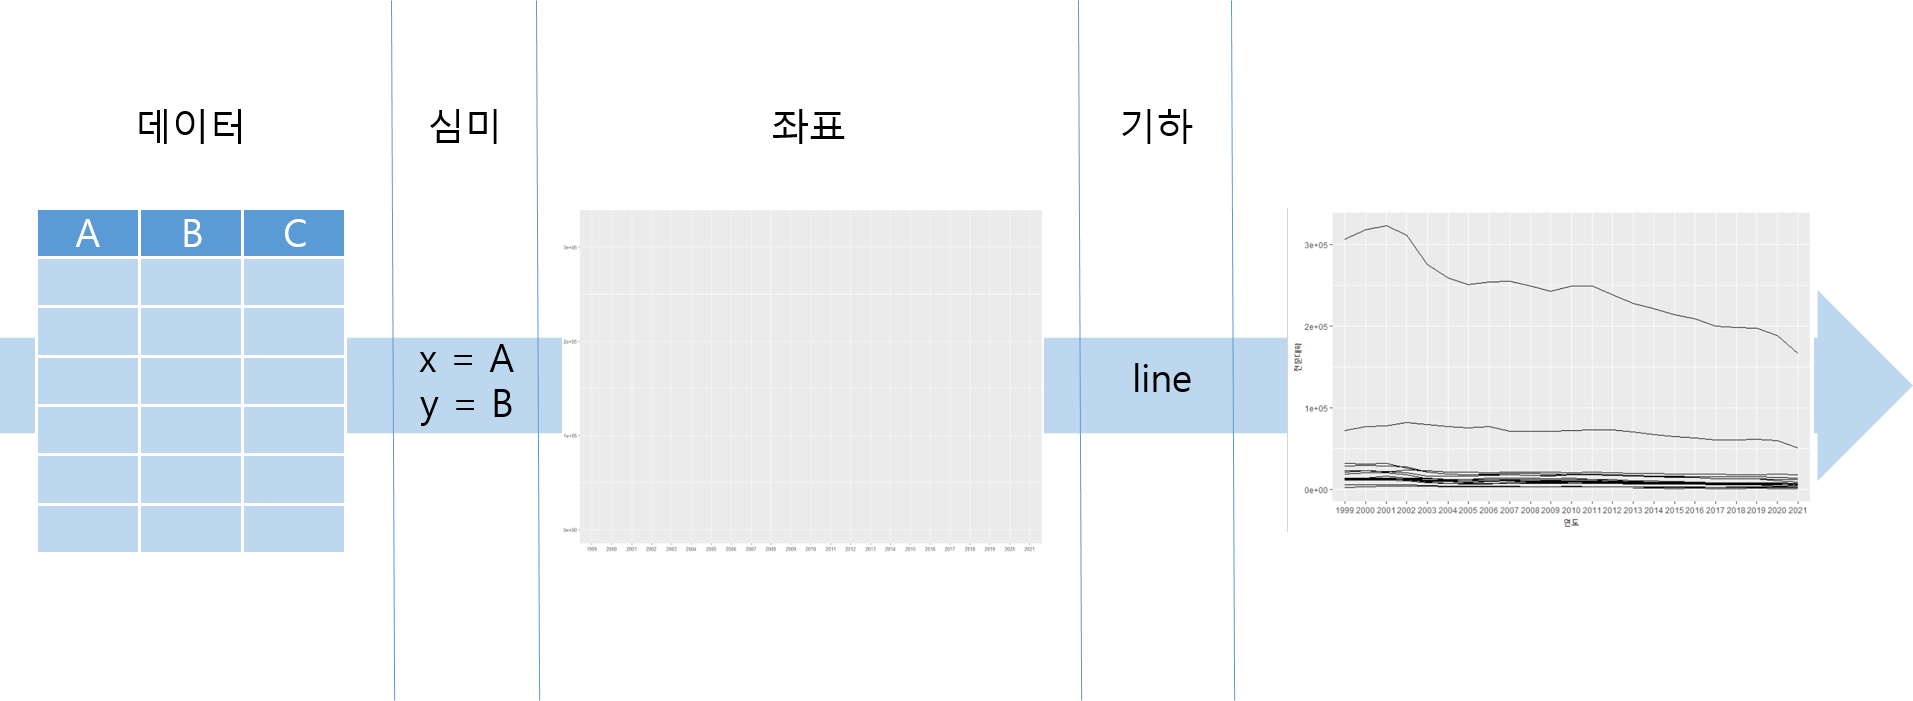
\includegraphics{그림1.png}\\
\texttt{ggplot2} 의 문법은 아래의 그림과 같다. 시작은 반드시 \texttt{ggplot()} 함수부터이다. 이후는 순서에 큰 영향은 없으나 일반적으로 \texttt{geom\_} 으로 시작하는 기하요소 함수를 사용하며 이 기하요소 함수 안에서 \texttt{aes()} 함수를 사용하여 미적 요소를 매핑한다. 각각의 기하요소에 공통적으로 적용될 미적요소의 매핑은 \texttt{ggplot()} 에 넣어 준다. \texttt{ggplot()} 를 사용하여 여러개의 레이어를 중첩하여 사용하기 위해서는 문법에서 제공하는 각각의 함수를 파이프가 아닌 \texttt{+} 기호 연결하여 사용한다.

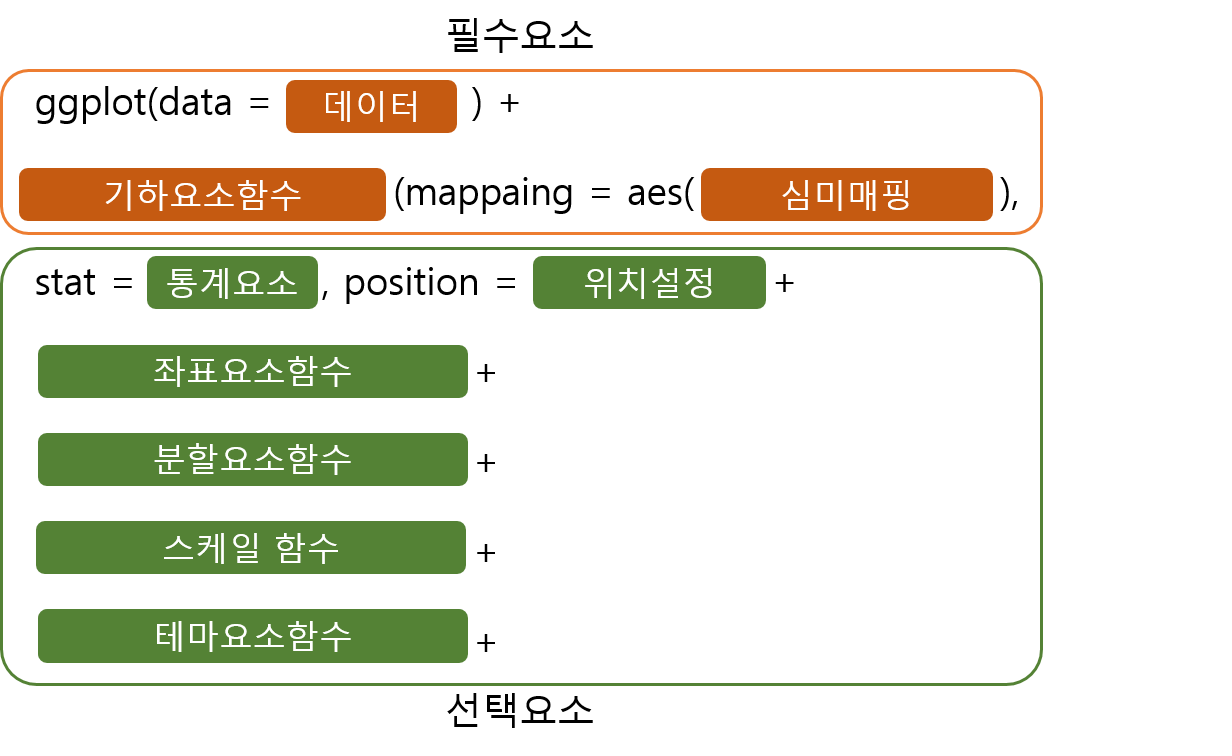
\includegraphics{그림2.png}

\hypertarget{ggplot}{%
\subsubsection{\texorpdfstring{2.1 \texttt{ggplot()}}{2.1 ggplot()}}\label{ggplot}}

\texttt{ggplot()} 는 \texttt{ggplot()} 객체를 만들기 위해 초기화하는 함수이다. \texttt{ggplot()} 은 시각화를 위한 대상 데이터를 선언하고 전체 레이어에서 공통적으로 사용될 미적 요소들을 지정하는데 사용된다. \texttt{ggplot()} 의 사용법과 주요 매개변수는 다음과 같다.

\begin{Shaded}
\begin{Highlighting}[]
\FunctionTok{ggplot}\NormalTok{(}\AttributeTok{data =} \ConstantTok{NULL}\NormalTok{, }\AttributeTok{mapping =} \FunctionTok{aes}\NormalTok{(), ...)}
  \SpecialCharTok{{-}}\NormalTok{ data }\SpecialCharTok{:}\NormalTok{ ggplot 객체를 위해 사용할 전체 레이어에 공통으로 사용될 기본 데이터프레임을 선언}
\StringTok{\textasciigrave{}}\AttributeTok{{-} mapping : aes()를 사용하여 전체 레이어에 공통으로 사용될 미적 요소 선언}
\end{Highlighting}
\end{Shaded}

\texttt{ggplot()} 에는 데이터에 연결된 기하요소가 선언되지 않기 때문에 데이터 시각화가 완전히 완성되지는 않는다. 하지만 데이터 미적요소의 매핑 결과는 볼 수 있다. 아래의 코드를 실행하면 앞 장에서 읽어들인 입학자 데이터를 X축과 Y축에 매핑한 결과를 볼 수 있다.

\begin{Shaded}
\begin{Highlighting}[]
\DocumentationTok{\#\# df\_입학자 데이터를 사용하여 x축은 연도열, y축은 전문대학열을 매핑하는 ggplot 객체 생성}
\FunctionTok{ggplot}\NormalTok{(df\_입학자, }\FunctionTok{aes}\NormalTok{(}\AttributeTok{x =}\NormalTok{ 연도, }\AttributeTok{y =}\NormalTok{ 전문대학))}
\end{Highlighting}
\end{Shaded}

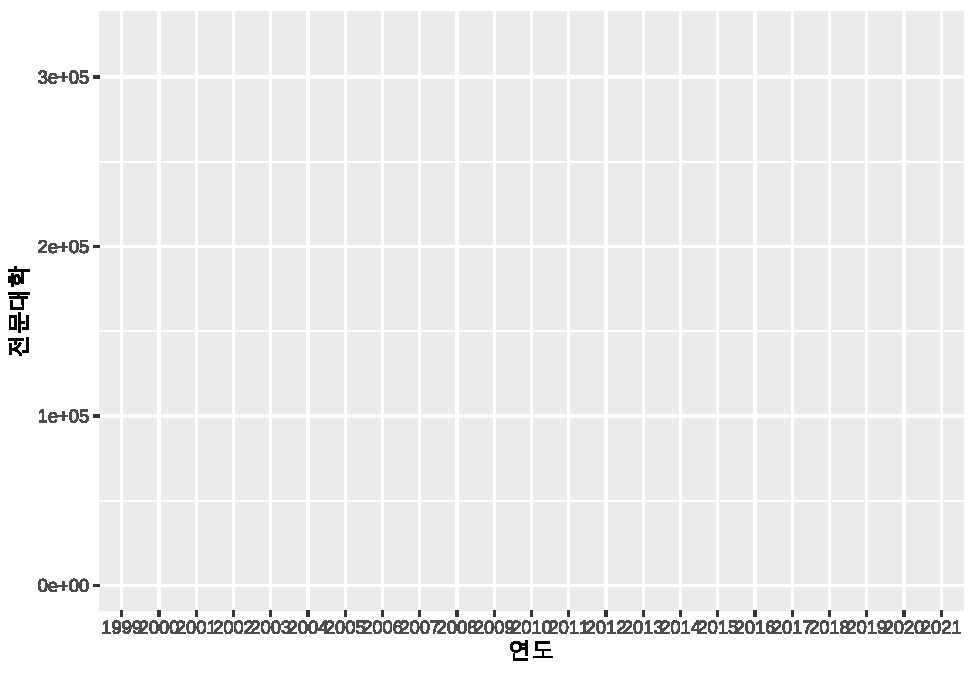
\includegraphics{chap3_files/figure-latex/unnamed-chunk-3-1.pdf}

위의 코드에서 사용된 \texttt{aes()} 는 미적요소을 매핑을 생성하는데 사용되는 함수이다. 미적요소 매핑은 어떤 데이터의 열(변수)가 어떤 시각화 요소들로 연결되는지를 선언하는 방법을 말한다. 위의 코드에서 \texttt{aes()} 에 \texttt{x} 시각화 요소중에 X축을 나타내는 매개변수인데 이 \texttt{x} 가 df\_입학자 데이터프레임의 연도열과 연결되었다. 또 \texttt{y} 는 시각화 요소 중 Y축을 나타내는 매개변수로 이 \texttt{y} 가 df\_입학자의 전문대학열과 연결되었다. 이 함수는 \texttt{ggplot()} 뿐아니라 기하요소를 정의하는 \texttt{geom\_*} 함수에서도 공통적으로 사용된다. \texttt{aes()} 의 사용법과 주요 매개변수는 다음과 같다.

\begin{Shaded}
\begin{Highlighting}[]
\FunctionTok{aes}\NormalTok{(x, y, ...)}
  \SpecialCharTok{{-}}\NormalTok{ x }\SpecialCharTok{:}\NormalTok{ X축에 매핑될 데이터 열}
  \SpecialCharTok{{-}}\NormalTok{ y }\SpecialCharTok{:}\NormalTok{ y축에 매핑될 데이터 열}
\end{Highlighting}
\end{Shaded}

앞서 설명한 바와 같이 \texttt{ggplot()} 에 선언되는 데이터와 미적 요소은 전체 \texttt{ggplot} 객체의 레이어에 공통으로 적용되는 데이터와 미적요소이다. \texttt{ggplot()} 에 선언되는 미적요소은 X축과 Y축의 매핑만 하는 것이 일반적이다. 모든 레이어에 공통적으로 적용되는 미적요소이 많지 않기 때문에 미리 정의해봐야 일부 레이어에서만 사용되기 떄문이다. 물론 \texttt{ggplot()} 에서 선언된 미적요소들이 각각의 레이어에서 다시 선언되는 경우에는 \texttt{ggplot()} 에서 선언된 데이터와 미적 요소보다 각각의 레이어에서 선언되는 데이터와 미적 요소이 해당 레이어에서 우선된다.

만약 모든 레이어에 공통적으로 적용되는 데이터나 미적 요소들이 없다면 매개변수 없이도 사용될 수 있고 데이터만 선언될 수도 있다. 하지만 데이터 선언없이 미적요소의 선언은 불가하다. 데이터가 없거나 미적요소이 없다면 아래와 같이 빈 \texttt{ggplot} 객체가 생성된다.

\begin{Shaded}
\begin{Highlighting}[]
\FunctionTok{ggplot}\NormalTok{(df\_입학자)}
\end{Highlighting}
\end{Shaded}


\includegraphics{chap3_files/figure-latex/unnamed-chunk-5-1.pdf}

\hypertarget{uxbbf8uxc801uxc694uxc18c}{%
\subsubsection{2.2 미적요소}\label{uxbbf8uxc801uxc694uxc18c}}

미적요소는 데이터를 표현하는데 사용되는 필요한 요소들을 통칭한다. 즉 미적요소로 지정할 수 있는 모든 요소은 \texttt{ggplot} 객체의 X, Y 좌표내에 표현되는 기하요소의 표현을 위한 요소들로 시각적 요소와 데이터 변수간의 매핑을 통해서 구현된다.

미적요소는 \texttt{aes()} 를 사용하여 매핑할 수 있고 고정값을 설정할 수 있다. 이 부분은 미적요소의 사용에 가장 혼동을 유발하는 부분이다. 미적요소를 매핑한다는 것은 미적요소가 데이터 변수에 의해 변경되어야 하는 경우 사용한다. 즉 미적요소가 변수에 대응됨으로써 변수의 변량에 따라 해당 미적요소들이 바뀌어서 표현된다. 그러나 고정값을 설정한다는 것은 변수에 대응되는 것이 아닌 특정값에 고정되도록 설정하기 때문에 고정값으로 설정된 기하요소들은 변수의 변량이 변경되어도 같은 미적요소로 표현된다. 미적요소는 사용하고자 하는 기하요소 함수(\texttt{geom\_*()}) 내에서 사용되지만 매핑할때는 반드시 \texttt{aes()} 함수를 사용하여 데이터 열이나 매핑 변수를 설정하여야 하고 고정값을 설정할 때는 반드시 \texttt{aes()} 함수 바깥에서 선언되어야 한다. 다음의 예를 살펴보자.

\begin{Shaded}
\begin{Highlighting}[]
\NormalTok{df\_입학자 }\SpecialCharTok{|}\ErrorTok{\textgreater{}} \FunctionTok{ggplot}\NormalTok{(}\FunctionTok{aes}\NormalTok{(}\AttributeTok{x =}\NormalTok{ 연도, }\AttributeTok{y =}\NormalTok{ 전문대학)) }\SpecialCharTok{+}
  \FunctionTok{geom\_point}\NormalTok{(}\FunctionTok{aes}\NormalTok{(}\AttributeTok{color =}\NormalTok{ 지역))}
\end{Highlighting}
\end{Shaded}

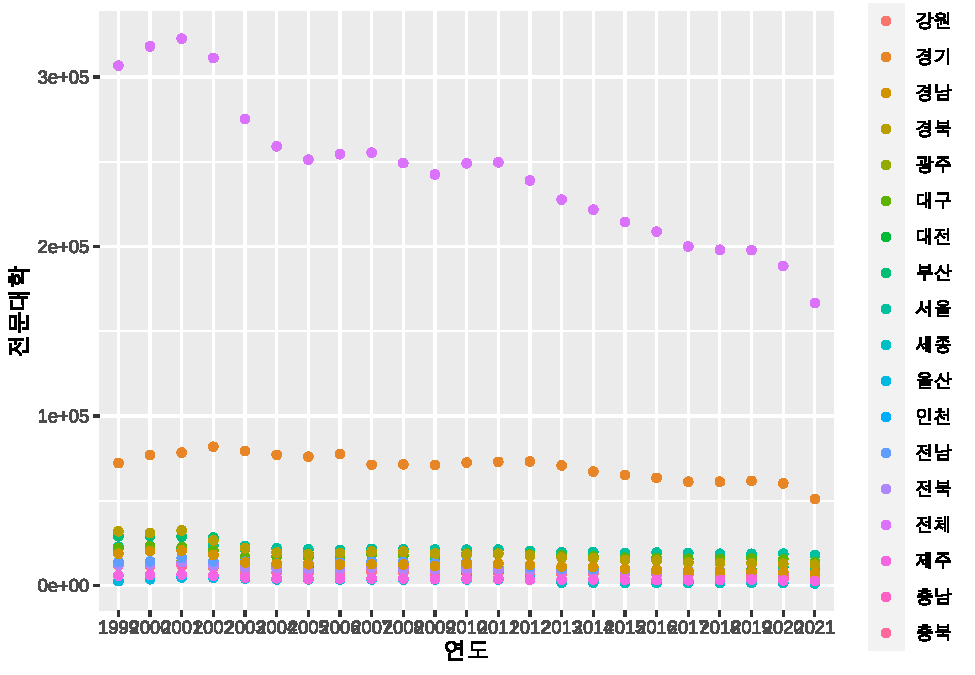
\includegraphics{chap3_files/figure-latex/unnamed-chunk-6-1.pdf}

\begin{Shaded}
\begin{Highlighting}[]
\NormalTok{df\_입학자 }\SpecialCharTok{|}\ErrorTok{\textgreater{}} \FunctionTok{ggplot}\NormalTok{(}\FunctionTok{aes}\NormalTok{(}\AttributeTok{x =}\NormalTok{ 연도, }\AttributeTok{y =}\NormalTok{ 전문대학)) }\SpecialCharTok{+}
  \FunctionTok{geom\_point}\NormalTok{(}\AttributeTok{color =} \StringTok{\textquotesingle{}red\textquotesingle{}}\NormalTok{)}
\end{Highlighting}
\end{Shaded}

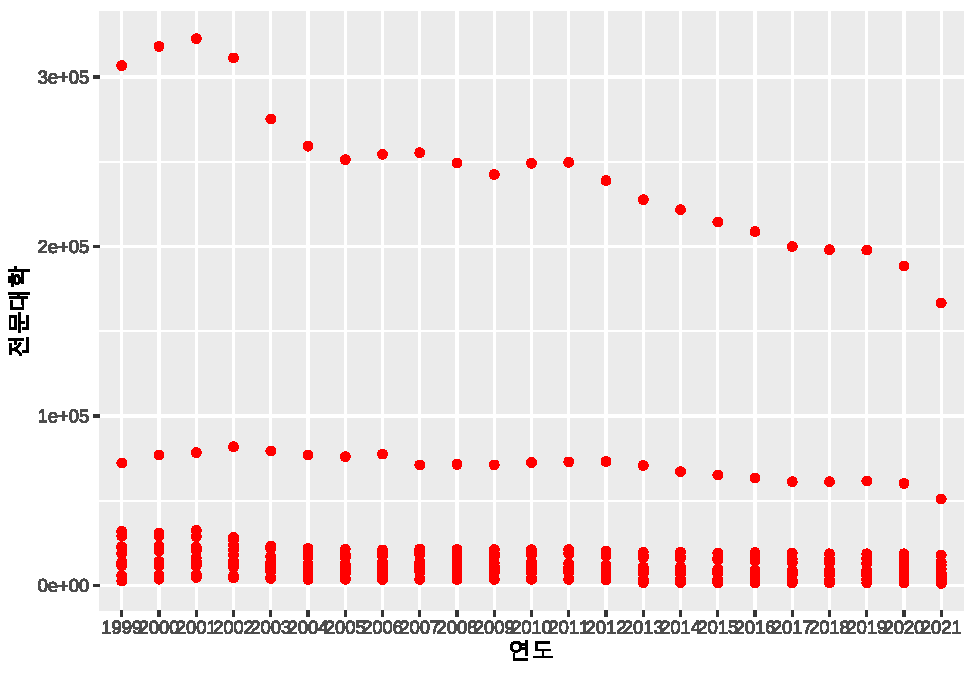
\includegraphics{chap3_files/figure-latex/unnamed-chunk-6-2.pdf}

위의 코드에서 차이는 \texttt{color} 미적요소이 \texttt{aes()} 내에 df\_입학자의 열이 매핑된 것과 \texttt{aes()} 밖에서 고정값(red)로 설정된 것이다. 결과에서 보이듯이 매핑된 \texttt{color} 는 지역 변수의 변량에 따라 \texttt{color} 가 자동적으로 바뀌어 데이터의 구분이 확연히 보인다. 반면 \texttt{aes()} 밖에서 고정값인 red값으로 설정된 코드는 전체 값들이 모두 red 값으로 표현되어 지역적으로 구분되지 않는다.

설정이 가능한 미적요소들은 다음과 같다.

\hypertarget{uxc704uxce58x-y-xend-yend}{%
\paragraph{2.2.1 위치(x , y, xend, yend)}\label{uxc704uxce58x-y-xend-yend}}

x와 y는 기하요소가 표시될 X축의 위치와 Y축의 위치 설정에 필요한 데이터 열의 매핑을 설정한다. 일부 선을 그리거나 사각형을 그리는 \texttt{geom\_segment()} 나 \texttt{geom\_rect()} 와 같은 기하요소 함수에서는 x, y 부터 시작하여 xend, yend까지 기하요소를 그린다. 다른 미적요소와는 달리 x, y, xend, yend는 매핑과 고정값 설정시 모두 반드시 \texttt{aes()} 함수안에서 사용되야 한다.

\hypertarget{color-colour}{%
\paragraph{2.2.2 color, colour}\label{color-colour}}

기하요소의 외곽선 색상을 설정한다. R에서 사용되는 색상은 색상 이름으로 설정하거나 RGB코드값으로 설정할 수 있다.

R에서 미리 정의된 색상 이름은 총 657개로 \texttt{colors()} 를 사용하면 확인이 가능하다.

\begin{Shaded}
\begin{Highlighting}[]
\DocumentationTok{\#\# R에서 미리 정의된 색상 이름 출력, 지면 관계상 10개만 출력}
\FunctionTok{colors}\NormalTok{() }\SpecialCharTok{|}\ErrorTok{\textgreater{}} \FunctionTok{head}\NormalTok{(}\DecValTok{10}\NormalTok{)}
\end{Highlighting}
\end{Shaded}

\begin{verbatim}
##  [1] "white"         "aliceblue"     "antiquewhite"  "antiquewhite1"
##  [5] "antiquewhite2" "antiquewhite3" "antiquewhite4" "aquamarine"   
##  [9] "aquamarine1"   "aquamarine2"
\end{verbatim}

RGB 색상 코드는 HTML/CSS에서와 같이 RGB 코드를 16진수 값(00에서 FF)을 사용하여 2자리씩 정의하는데 ``\#'' 접두사로 붙은 문자열로 설정한다. 예를 들어 red는은 ``\#FF0000''으로 표현된다.

\begin{Shaded}
\begin{Highlighting}[]
\DocumentationTok{\#\# df\_입학자의 지역이 \textquotesingle{}전체\textquotesingle{}인 데이터를 시각화하는데 막대의 외곽선 색상을 빨강으로 설정}
\NormalTok{df\_입학자 }\SpecialCharTok{|}\ErrorTok{\textgreater{}} \FunctionTok{filter}\NormalTok{(지역 }\SpecialCharTok{==} \StringTok{\textquotesingle{}전체\textquotesingle{}}\NormalTok{) }\SpecialCharTok{|}\ErrorTok{\textgreater{}}
  \FunctionTok{ggplot}\NormalTok{(}\FunctionTok{aes}\NormalTok{(}\AttributeTok{x =}\NormalTok{ 연도, }\AttributeTok{y =}\NormalTok{ 전문대학)) }\SpecialCharTok{+}
  \FunctionTok{geom\_col}\NormalTok{(}\AttributeTok{color =} \StringTok{\textquotesingle{}\#ff0000\textquotesingle{}}\NormalTok{)}
\end{Highlighting}
\end{Shaded}

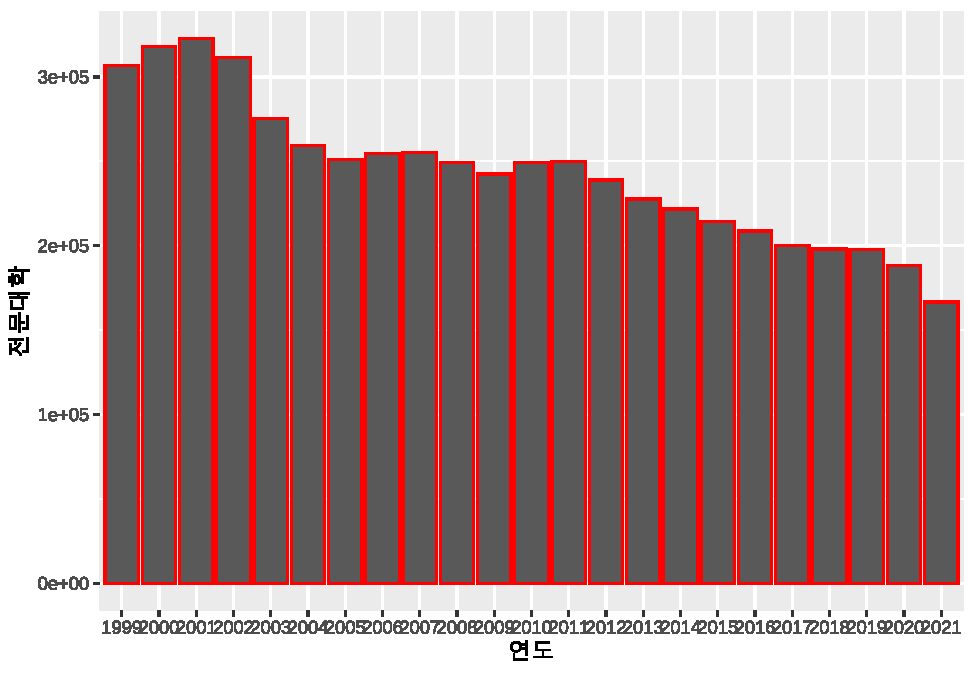
\includegraphics{chap3_files/figure-latex/unnamed-chunk-8-1.pdf}

\hypertarget{fill}{%
\paragraph{2.2.3 fill}\label{fill}}

기하요소의 내부 색상의 설정을 설정한다. 색상의 설정은 \texttt{color} 설정과 동일하다.

\begin{Shaded}
\begin{Highlighting}[]
\DocumentationTok{\#\# df\_입학자의 지역이 \textquotesingle{}전체\textquotesingle{}인 데이터를 시각화하는데 막대의 내부 색상을 빨강으로 설정}
\NormalTok{df\_입학자 }\SpecialCharTok{|}\ErrorTok{\textgreater{}} \FunctionTok{filter}\NormalTok{(지역 }\SpecialCharTok{==} \StringTok{\textquotesingle{}전체\textquotesingle{}}\NormalTok{) }\SpecialCharTok{|}\ErrorTok{\textgreater{}}
  \FunctionTok{ggplot}\NormalTok{(}\FunctionTok{aes}\NormalTok{(}\AttributeTok{x =}\NormalTok{ 연도, }\AttributeTok{y =}\NormalTok{ 전문대학)) }\SpecialCharTok{+}
  \FunctionTok{geom\_col}\NormalTok{(}\AttributeTok{fill =} \StringTok{\textquotesingle{}\#ff0000\textquotesingle{}}\NormalTok{)}
\end{Highlighting}
\end{Shaded}

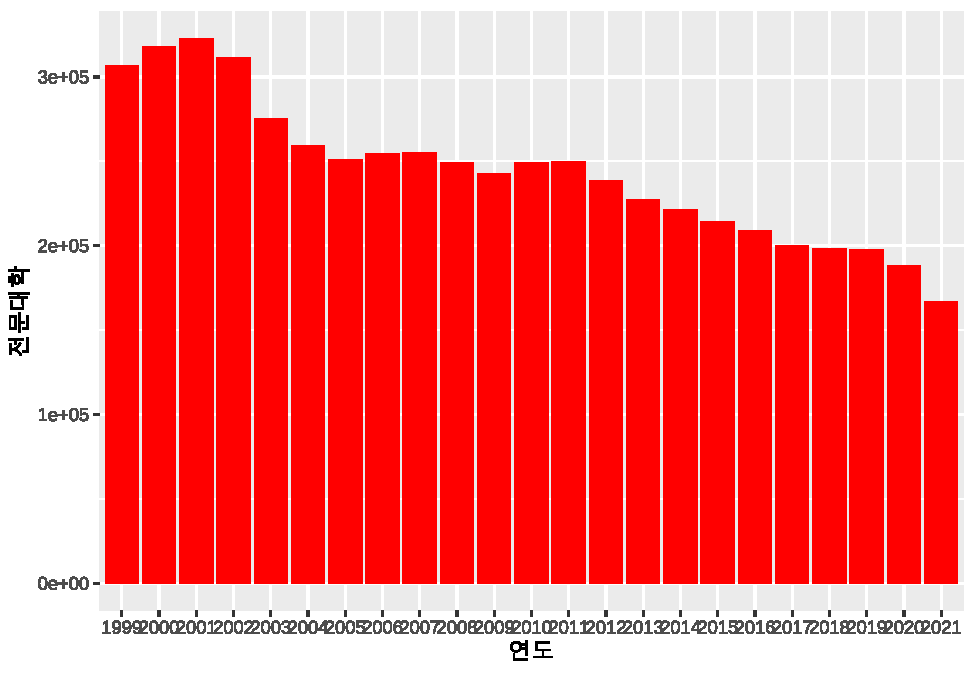
\includegraphics{chap3_files/figure-latex/unnamed-chunk-9-1.pdf}

\hypertarget{alpha}{%
\paragraph{2.2.4 alpha}\label{alpha}}

기하요소의 투명도를 설정한다. \texttt{alpha} 는 정수형 수치로 설정하는데 0부터 1사이의 값을 가진다. 0에 가까울수록 투명해지고 1에 가까울 수록 불투명해진다.

\begin{Shaded}
\begin{Highlighting}[]
\DocumentationTok{\#\# df\_입학자의 지역이 \textquotesingle{}전체\textquotesingle{}인 데이터를 시각화하는데 막대의 투명도를 0.3으로 설정}
\NormalTok{df\_입학자 }\SpecialCharTok{|}\ErrorTok{\textgreater{}} \FunctionTok{filter}\NormalTok{(지역 }\SpecialCharTok{==} \StringTok{\textquotesingle{}전체\textquotesingle{}}\NormalTok{) }\SpecialCharTok{|}\ErrorTok{\textgreater{}}
  \FunctionTok{ggplot}\NormalTok{(}\FunctionTok{aes}\NormalTok{(}\AttributeTok{x =}\NormalTok{ 연도, }\AttributeTok{y =}\NormalTok{ 전문대학)) }\SpecialCharTok{+}
  \FunctionTok{geom\_col}\NormalTok{(}\AttributeTok{alpha =} \FloatTok{0.3}\NormalTok{)}
\end{Highlighting}
\end{Shaded}

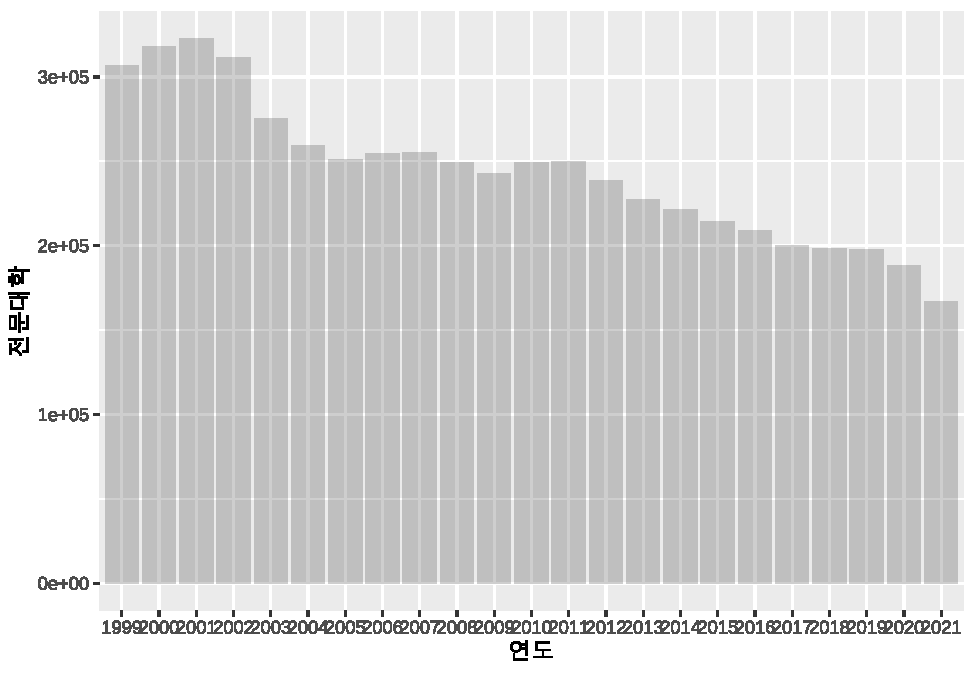
\includegraphics{chap3_files/figure-latex/unnamed-chunk-10-1.pdf}

\begin{Shaded}
\begin{Highlighting}[]
\DocumentationTok{\#\# df\_입학자의 지역이 \textquotesingle{}전체\textquotesingle{}인 데이터를 시각화하는데 막대의 투명도를 0.7로 설정}
\NormalTok{df\_입학자 }\SpecialCharTok{|}\ErrorTok{\textgreater{}} \FunctionTok{filter}\NormalTok{(지역 }\SpecialCharTok{==} \StringTok{\textquotesingle{}전체\textquotesingle{}}\NormalTok{) }\SpecialCharTok{|}\ErrorTok{\textgreater{}}
  \FunctionTok{ggplot}\NormalTok{(}\FunctionTok{aes}\NormalTok{(}\AttributeTok{x =}\NormalTok{ 연도, }\AttributeTok{y =}\NormalTok{ 전문대학)) }\SpecialCharTok{+}
  \FunctionTok{geom\_col}\NormalTok{(}\AttributeTok{alpha =} \FloatTok{0.7}\NormalTok{)}
\end{Highlighting}
\end{Shaded}

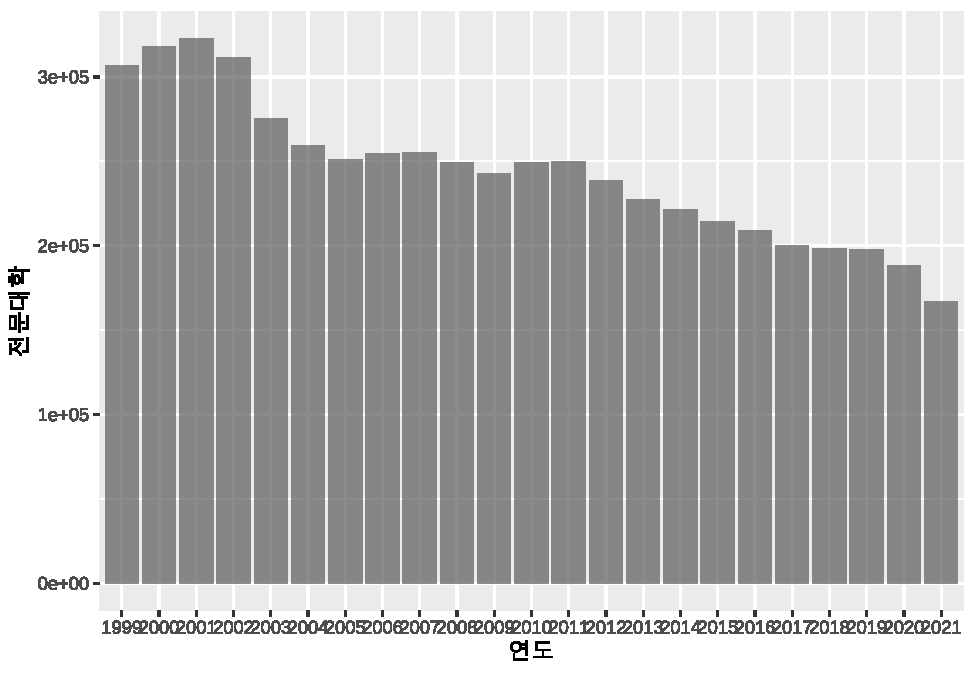
\includegraphics{chap3_files/figure-latex/unnamed-chunk-10-2.pdf}

\hypertarget{linetype}{%
\paragraph{2.2.5 linetype}\label{linetype}}

기하요소 중 선으로 그려지는 기하 요소의 선 타입을 결정한다. R에서는 총 7가지의 선 타입을 제공하는데 0부터 6까지의 숫자나 선 타입의 이름을 사용하여 설정할 수 있다.

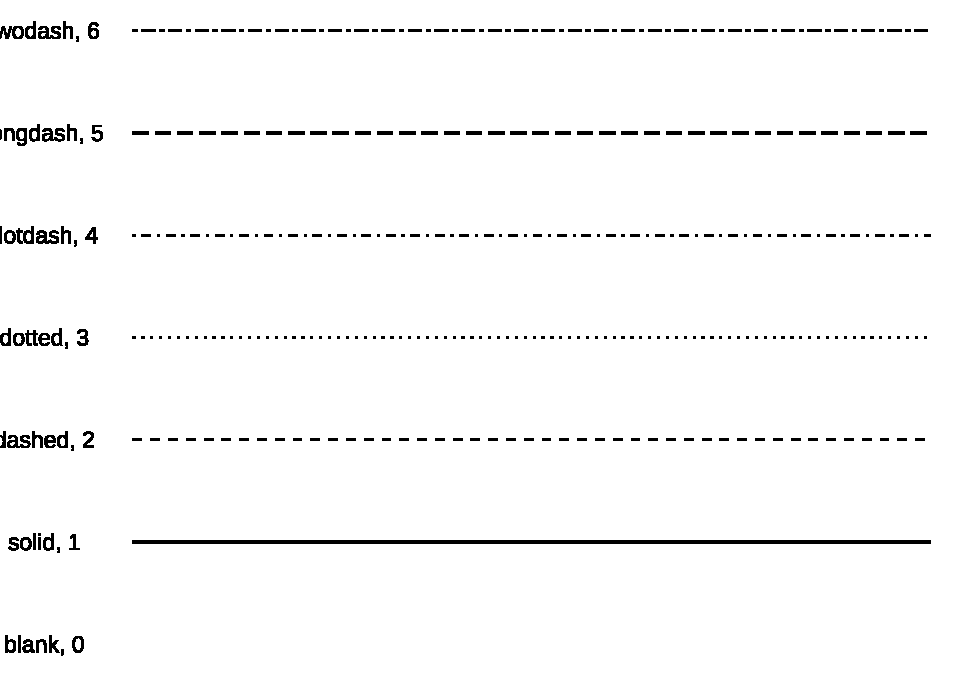
\includegraphics{chap3_files/figure-latex/unnamed-chunk-11-1.pdf}

\begin{Shaded}
\begin{Highlighting}[]
\DocumentationTok{\#\# df\_입학자의 지역이 \textquotesingle{}전체\textquotesingle{}인 데이터를 시각화하는데 선의 타입을 \textquotesingle{}dashed\textquotesingle{}로 설정}
\NormalTok{df\_입학자 }\SpecialCharTok{|}\ErrorTok{\textgreater{}} \FunctionTok{filter}\NormalTok{(지역 }\SpecialCharTok{==} \StringTok{\textquotesingle{}전체\textquotesingle{}}\NormalTok{) }\SpecialCharTok{|}\ErrorTok{\textgreater{}}
  \FunctionTok{ggplot}\NormalTok{(}\FunctionTok{aes}\NormalTok{(}\AttributeTok{x =}\NormalTok{ 연도, }\AttributeTok{y =}\NormalTok{ 전문대학)) }\SpecialCharTok{+}
  \FunctionTok{geom\_line}\NormalTok{(}\FunctionTok{aes}\NormalTok{(}\AttributeTok{group =} \DecValTok{1}\NormalTok{), }\AttributeTok{linetype =} \StringTok{\textquotesingle{}dotted\textquotesingle{}}\NormalTok{)}
\end{Highlighting}
\end{Shaded}

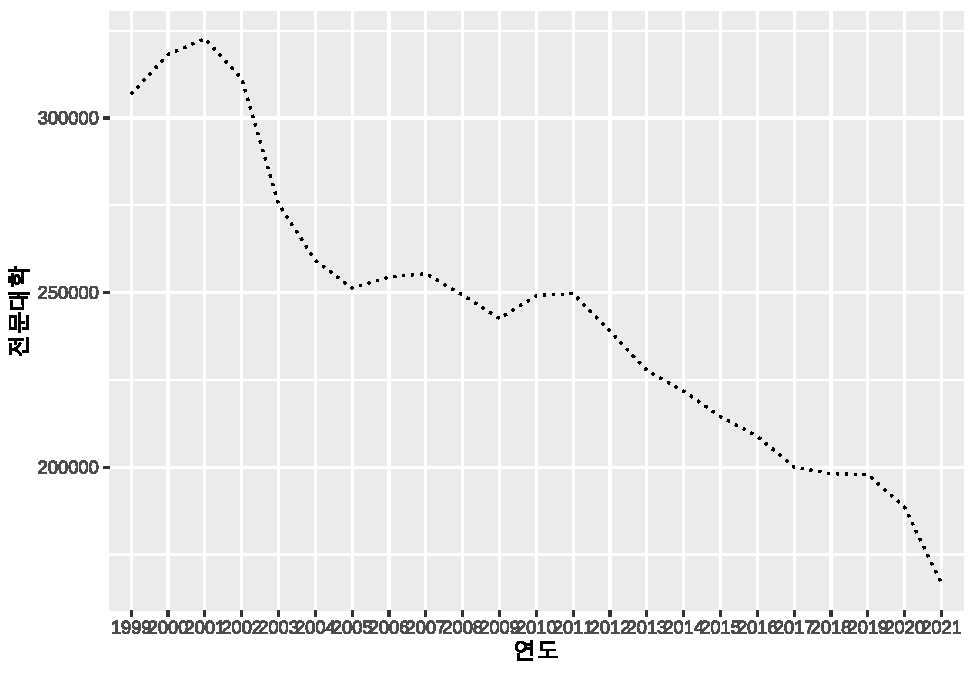
\includegraphics{chap3_files/figure-latex/unnamed-chunk-12-1.pdf}

\hypertarget{size}{%
\paragraph{2.2.6 size}\label{size}}

\texttt{size} 는 기하요소의 크기를 설정한다. 기하요소가 점이면 점의 크기, 선이면 선의 굵기를 설정한다. 점의 크기를 결정할 때는 반지름의 길이를 밀리미터 단위로 지정한다. 또 선의 굵기도 밀리미터 단위로 지정할 수 있다.

\begin{Shaded}
\begin{Highlighting}[]
\DocumentationTok{\#\# df\_입학자의 지역이 \textquotesingle{}전체\textquotesingle{}인 데이터를 시각화하는데 선의 크기를 3으로 설정}
\NormalTok{df\_입학자 }\SpecialCharTok{|}\ErrorTok{\textgreater{}} \FunctionTok{filter}\NormalTok{(지역 }\SpecialCharTok{==} \StringTok{\textquotesingle{}전체\textquotesingle{}}\NormalTok{) }\SpecialCharTok{|}\ErrorTok{\textgreater{}}
  \FunctionTok{ggplot}\NormalTok{(}\FunctionTok{aes}\NormalTok{(}\AttributeTok{x =}\NormalTok{ 연도, }\AttributeTok{y =}\NormalTok{ 전문대학)) }\SpecialCharTok{+}
  \FunctionTok{geom\_line}\NormalTok{(}\FunctionTok{aes}\NormalTok{(}\AttributeTok{group =} \DecValTok{1}\NormalTok{), }\AttributeTok{size =} \DecValTok{3}\NormalTok{)}
\end{Highlighting}
\end{Shaded}

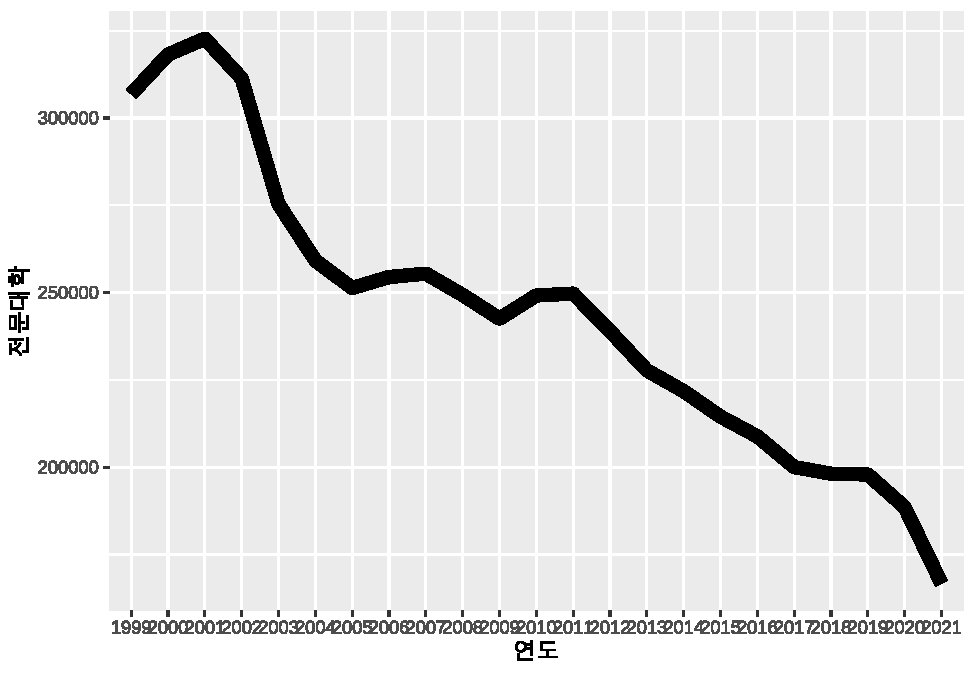
\includegraphics{chap3_files/figure-latex/unnamed-chunk-13-1.pdf}

\begin{Shaded}
\begin{Highlighting}[]
\DocumentationTok{\#\# df\_입학자의 지역이 \textquotesingle{}전체\textquotesingle{}인 데이터를 시각화하는데 점의 크기를 3으로 설정}
\NormalTok{df\_입학자 }\SpecialCharTok{|}\ErrorTok{\textgreater{}} \FunctionTok{filter}\NormalTok{(지역 }\SpecialCharTok{==} \StringTok{\textquotesingle{}전체\textquotesingle{}}\NormalTok{) }\SpecialCharTok{|}\ErrorTok{\textgreater{}}
  \FunctionTok{ggplot}\NormalTok{(}\FunctionTok{aes}\NormalTok{(}\AttributeTok{x =}\NormalTok{ 연도, }\AttributeTok{y =}\NormalTok{ 전문대학)) }\SpecialCharTok{+}
  \FunctionTok{geom\_point}\NormalTok{(}\AttributeTok{size =} \DecValTok{3}\NormalTok{)}
\end{Highlighting}
\end{Shaded}

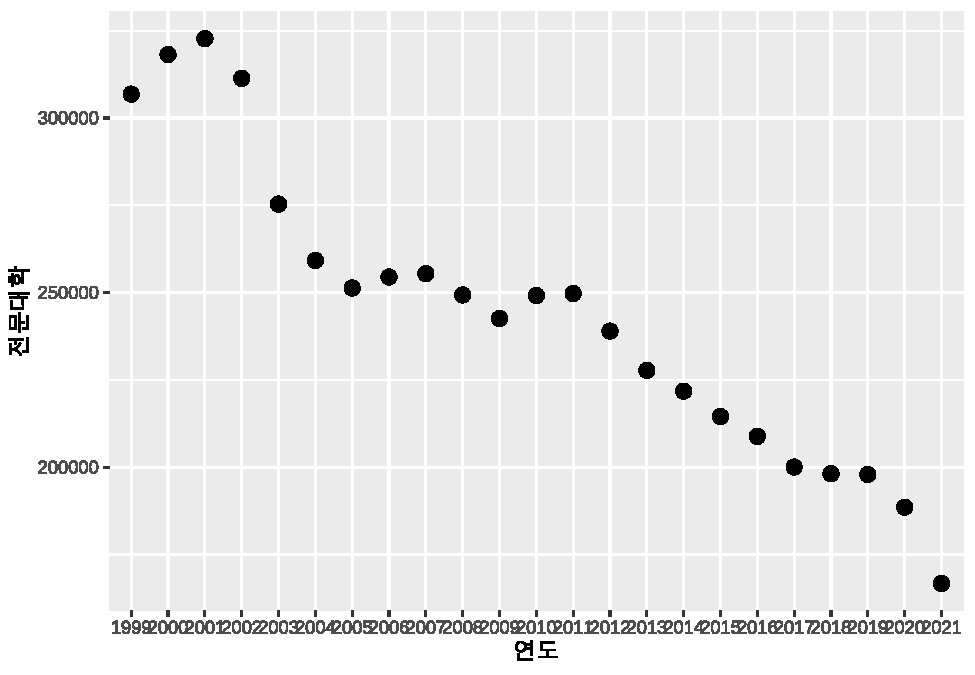
\includegraphics{chap3_files/figure-latex/unnamed-chunk-13-2.pdf}

\hypertarget{shape}{%
\paragraph{2.2.7 shape}\label{shape}}

\texttt{shape} 는 기하요소가 점일때 점의 모양을 표현하는 미적요소이다. R에서는 점을 표현하는 기하요소를 25가지 지원한다. 앞선 라인타입과 유사하게 번호로 표현할 수도 있고 사전에 정의된 \texttt{shape} 이름을 사용할 수도 있다. 다음은 R에서 제공하는 \texttt{shape}이다.

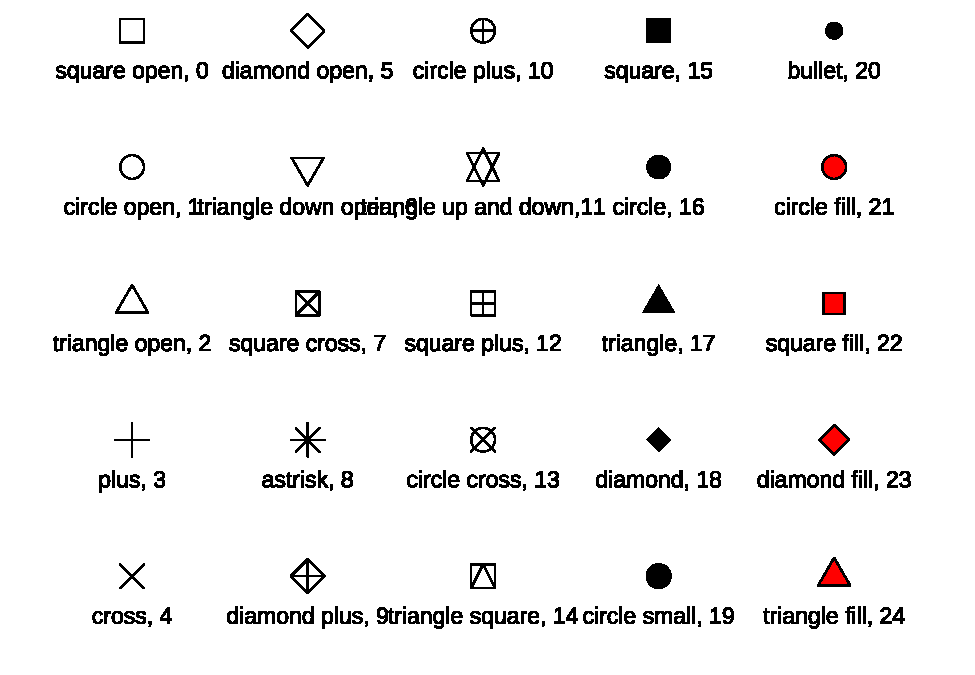
\includegraphics{chap3_files/figure-latex/unnamed-chunk-14-1.pdf}

위의 \texttt{shape}를 실제 사용하는 예제는 다음과 같다.

\begin{Shaded}
\begin{Highlighting}[]
\DocumentationTok{\#\# df\_입학자의 지역이 \textquotesingle{}전체\textquotesingle{}인 데이터를 시각화하는데 점의 모양을 15로 설정}
\NormalTok{df\_입학자 }\SpecialCharTok{|}\ErrorTok{\textgreater{}} \FunctionTok{filter}\NormalTok{(지역 }\SpecialCharTok{==} \StringTok{\textquotesingle{}전체\textquotesingle{}}\NormalTok{) }\SpecialCharTok{|}\ErrorTok{\textgreater{}}
  \FunctionTok{ggplot}\NormalTok{(}\FunctionTok{aes}\NormalTok{(}\AttributeTok{x =}\NormalTok{ 연도, }\AttributeTok{y =}\NormalTok{ 전문대학)) }\SpecialCharTok{+}
  \FunctionTok{geom\_point}\NormalTok{(}\AttributeTok{shape =} \DecValTok{15}\NormalTok{)}
\end{Highlighting}
\end{Shaded}

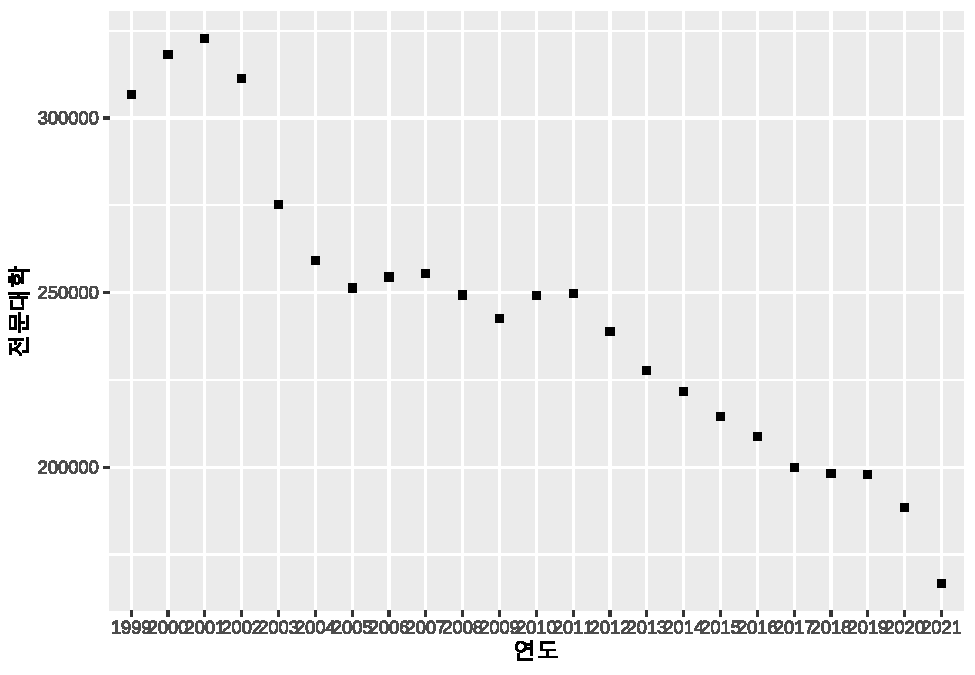
\includegraphics{chap3_files/figure-latex/unnamed-chunk-15-1.pdf}

\begin{Shaded}
\begin{Highlighting}[]
\DocumentationTok{\#\# df\_입학자의 지역이 \textquotesingle{}전체\textquotesingle{}인 데이터를 시각화하는데 점의 모양을 \textquotesingle{}triangle open\textquotesingle{}으로 설정}
\NormalTok{df\_입학자 }\SpecialCharTok{|}\ErrorTok{\textgreater{}} \FunctionTok{filter}\NormalTok{(지역 }\SpecialCharTok{==} \StringTok{\textquotesingle{}전체\textquotesingle{}}\NormalTok{) }\SpecialCharTok{|}\ErrorTok{\textgreater{}}
  \FunctionTok{ggplot}\NormalTok{(}\FunctionTok{aes}\NormalTok{(}\AttributeTok{x =}\NormalTok{ 연도, }\AttributeTok{y =}\NormalTok{ 전문대학)) }\SpecialCharTok{+}
  \FunctionTok{geom\_point}\NormalTok{(}\AttributeTok{shape =} \StringTok{\textquotesingle{}triangle open\textquotesingle{}}\NormalTok{)}
\end{Highlighting}
\end{Shaded}

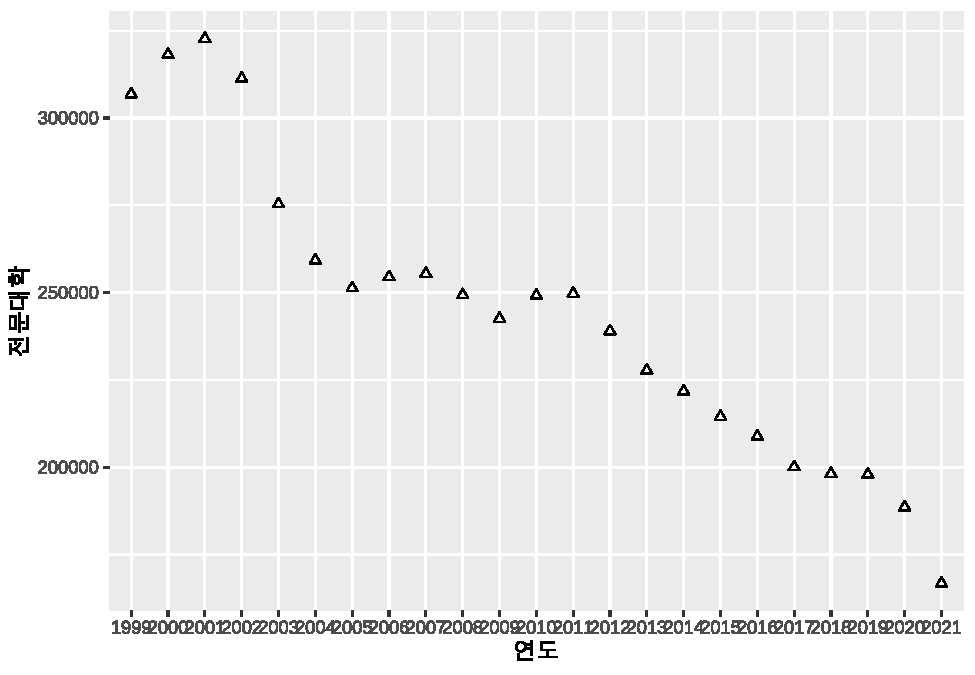
\includegraphics{chap3_files/figure-latex/unnamed-chunk-15-2.pdf}

\hypertarget{label}{%
\paragraph{2.2.8 label}\label{label}}

\texttt{label}은 텍스트로 표현되는 기하요소를 말한다. 데이터의 위치에 대한 수치값을 표현한다거나 데이터의 분류에 대한 문자를 표현할 때 사용되는 미적요소이다. \texttt{label}은 주로 텍스트에 관련된 기하요소인 \texttt{geom\_text()}나 \texttt{geom\_label()}에서 주로 사용된다.

\begin{Shaded}
\begin{Highlighting}[]
\DocumentationTok{\#\# df\_입학자의 지역이 \textquotesingle{}전체\textquotesingle{}인 데이터를 시각화하는데 라벨을 \textquotesingle{}전문대학\textquotesingle{}으로 설정}
\NormalTok{df\_입학자 }\SpecialCharTok{|}\ErrorTok{\textgreater{}} \FunctionTok{filter}\NormalTok{(지역 }\SpecialCharTok{==} \StringTok{\textquotesingle{}전체\textquotesingle{}}\NormalTok{) }\SpecialCharTok{|}\ErrorTok{\textgreater{}}
  \FunctionTok{ggplot}\NormalTok{(}\FunctionTok{aes}\NormalTok{(}\AttributeTok{x =}\NormalTok{ 연도, }\AttributeTok{y =}\NormalTok{ 전문대학)) }\SpecialCharTok{+}
  \FunctionTok{geom\_text}\NormalTok{(}\AttributeTok{label =} \StringTok{\textquotesingle{}전문대학\textquotesingle{}}\NormalTok{)}
\end{Highlighting}
\end{Shaded}

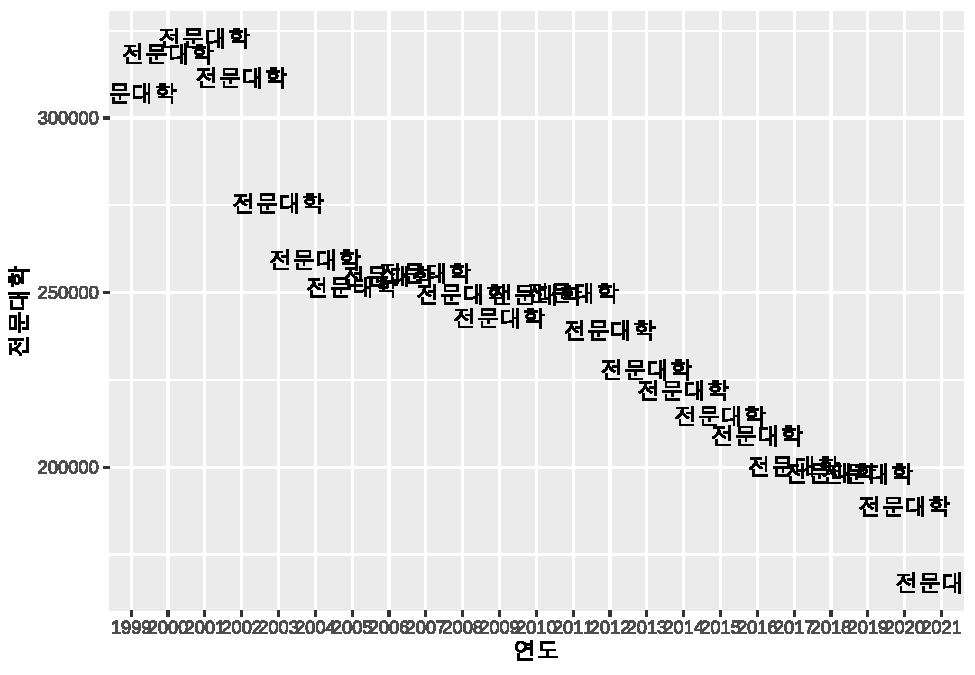
\includegraphics{chap3_files/figure-latex/unnamed-chunk-16-1.pdf}

\begin{Shaded}
\begin{Highlighting}[]
\DocumentationTok{\#\# df\_입학자의 지역이 \textquotesingle{}전체\textquotesingle{}인 데이터를 시각화하는데 라벨을 \textquotesingle{}전문대학\textquotesingle{}열에 매핑}
\NormalTok{df\_입학자 }\SpecialCharTok{|}\ErrorTok{\textgreater{}} \FunctionTok{filter}\NormalTok{(지역 }\SpecialCharTok{==} \StringTok{\textquotesingle{}전체\textquotesingle{}}\NormalTok{) }\SpecialCharTok{|}\ErrorTok{\textgreater{}}
  \FunctionTok{ggplot}\NormalTok{(}\FunctionTok{aes}\NormalTok{(}\AttributeTok{x =}\NormalTok{ 연도, }\AttributeTok{y =}\NormalTok{ 전문대학)) }\SpecialCharTok{+}
  \FunctionTok{geom\_text}\NormalTok{(}\FunctionTok{aes}\NormalTok{(}\AttributeTok{label =}\NormalTok{ 전문대학))}
\end{Highlighting}
\end{Shaded}

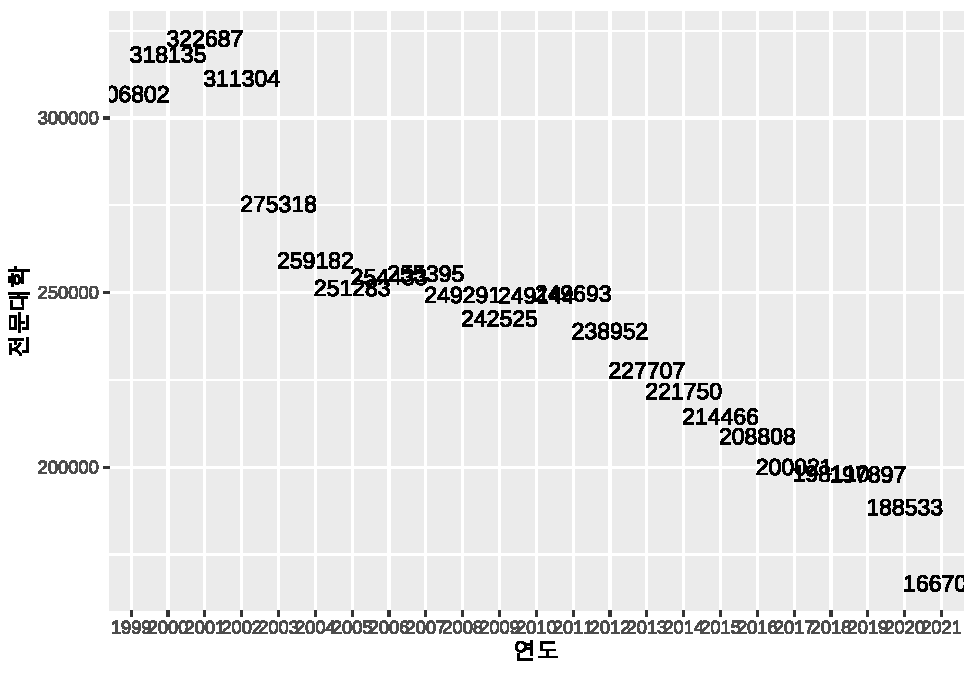
\includegraphics{chap3_files/figure-latex/unnamed-chunk-16-2.pdf}

\hypertarget{group}{%
\paragraph{2.2.9 group}\label{group}}

기하요소는 개별(individual) 기하요소와 집합(collective) 기하요소로 구분될 수 있다. 개별 기하요소는 각각의 관측이(행)을 각각의 기하요소로 매핑해서 표현하지만 집합 기하요소는 여러개의 관측치를 하나의 기하요소로 표현한다.\footnote{Hadley Wickham, ggplot2:Elegant Graphics for Data Analysis 2nd edition, P 46, Springer, 2016.} 집합 기하요소는 통계적인 요약이 필요한 Box Plot이나 한번에 여러개의 변량이 연결되어 표현되야하는 도형(polygon), 선, 세그먼트 등에서 연결되는 구분이 설정되어야한다. 이를 표현하기 위해 사용되는 미적요소가 \texttt{group}이다. 설명한대로 \texttt{group} 은 직접적으로 표현되는 미적요소는 아니지만 미적요소가 적용되는 범위를 설정하기 위해 사용되는 미적요소이다.

아래의 코드를 살펴보자.

\begin{Shaded}
\begin{Highlighting}[]
\DocumentationTok{\#\# df\_입학자 중 전문대학 입학생을 선 그래프로 시각화하는데 지역별 구분이 되지 않음}
\NormalTok{df\_입학자 }\SpecialCharTok{|}\ErrorTok{\textgreater{}}
  \FunctionTok{ggplot}\NormalTok{(}\FunctionTok{aes}\NormalTok{(}\AttributeTok{x =}\NormalTok{ 연도, }\AttributeTok{y =}\NormalTok{ 전문대학)) }\SpecialCharTok{+}
  \FunctionTok{geom\_line}\NormalTok{(}\FunctionTok{aes}\NormalTok{(}\AttributeTok{color =}\NormalTok{ 지역))}
\end{Highlighting}
\end{Shaded}

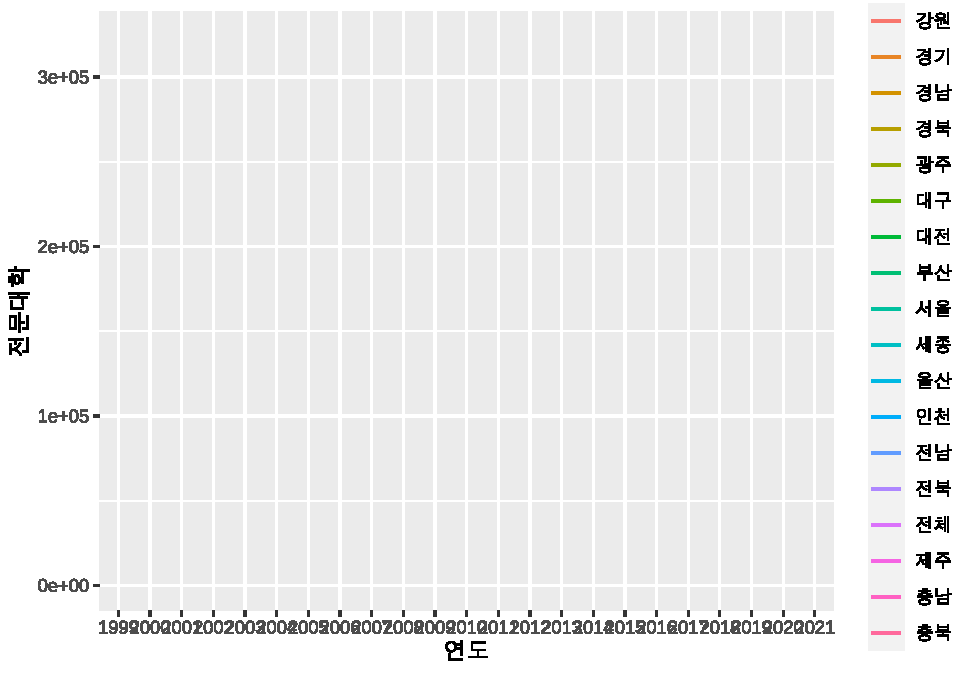
\includegraphics{chap3_files/figure-latex/unnamed-chunk-17-1.pdf}

\begin{Shaded}
\begin{Highlighting}[]
\DocumentationTok{\#\# df\_입학자 중 전문대학 입학생을 선 그래프로 시각화하는데 group을 지역으로 설정함으로써 지역별 구분이 가능}
\NormalTok{df\_입학자 }\SpecialCharTok{|}\ErrorTok{\textgreater{}}
  \FunctionTok{ggplot}\NormalTok{(}\FunctionTok{aes}\NormalTok{(}\AttributeTok{x =}\NormalTok{ 연도, }\AttributeTok{y =}\NormalTok{ 전문대학)) }\SpecialCharTok{+}
  \FunctionTok{geom\_line}\NormalTok{(}\FunctionTok{aes}\NormalTok{(}\AttributeTok{color =}\NormalTok{ 지역, }\AttributeTok{group =}\NormalTok{ 지역))}
\end{Highlighting}
\end{Shaded}

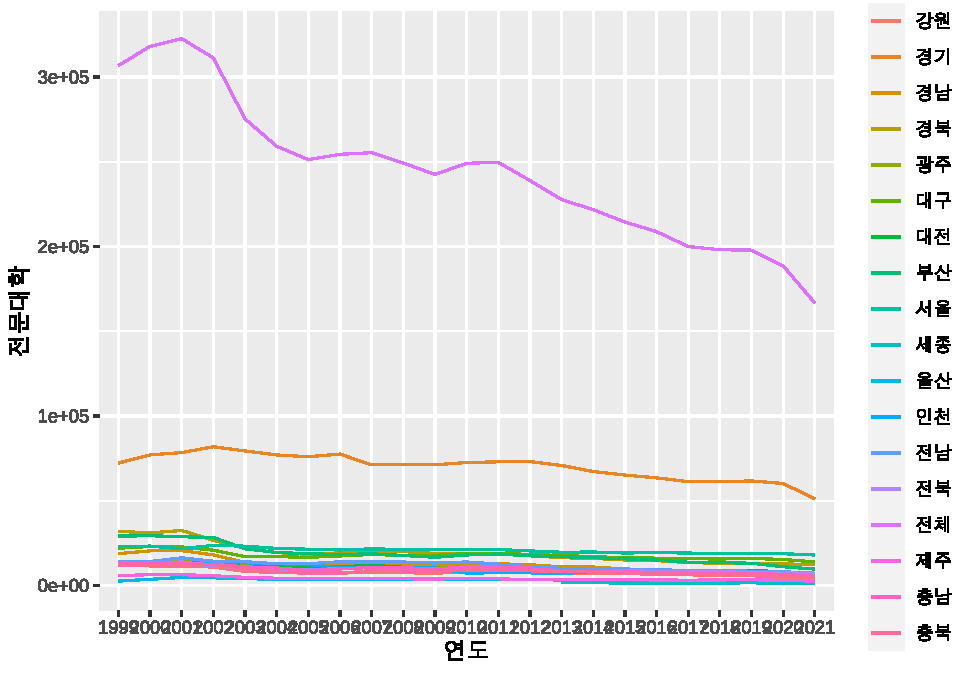
\includegraphics{chap3_files/figure-latex/unnamed-chunk-17-2.pdf}

위의 코드에서 앞선 코드는 \texttt{group} 을 지정하지 않고 \texttt{color} 만 df\_입학자 데이터의 지역열에 매핑하였다. 하지만 선으로 표현될 미적요소는 지역별로 그루핑되어야 정상적으로 표현되는데 단지 \texttt{color} 만의 매핑으로는 정상적으로 표현되지 않는다. 따라서 \texttt{geom\_line()} 으로 여러개의 선이 표현되는 선 그래프를 표현하기 해서는 반드시 \texttt{group} 으로 그루핑되는 열을 지정해야 정상적으로 표현된다.

그렇다면 단 하나의 선만이 있는 선 그래프는 어떻게 될까? 단 하나의 선이기 때문에 \texttt{group} 이 필요없을까? 답은 그렇지 않다. 다만 단 하나의 선이 있는 경우에는 \texttt{group\ =\ 1} 로 선언함으로써 열을 매핑하지 않고 사용할 수도 있다.

\begin{Shaded}
\begin{Highlighting}[]
\DocumentationTok{\#\# df\_입학자 중 지역이 전체에 해당하는 전문대학 입학생을 선 그래프로 시각화하는데 지역이 하나뿐이므로 group을 1로 설정함으로써 선그래프를 그릴 수 있음}
\NormalTok{df\_입학자 }\SpecialCharTok{|}\ErrorTok{\textgreater{}} \FunctionTok{filter}\NormalTok{(지역 }\SpecialCharTok{==} \StringTok{\textquotesingle{}전체\textquotesingle{}}\NormalTok{) }\SpecialCharTok{|}\ErrorTok{\textgreater{}}
  \FunctionTok{ggplot}\NormalTok{(}\FunctionTok{aes}\NormalTok{(}\AttributeTok{x =}\NormalTok{ 연도, }\AttributeTok{y =}\NormalTok{ 전문대학)) }\SpecialCharTok{+}
  \FunctionTok{geom\_line}\NormalTok{(}\FunctionTok{aes}\NormalTok{(}\AttributeTok{color =}\NormalTok{ 지역, }\AttributeTok{group =} \DecValTok{1}\NormalTok{))}
\end{Highlighting}
\end{Shaded}

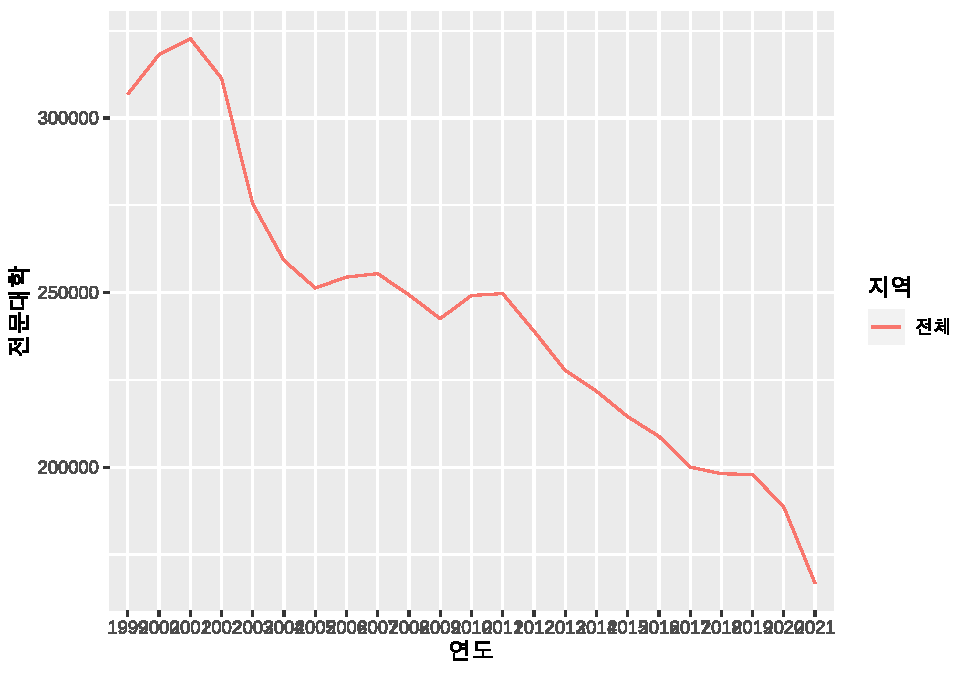
\includegraphics{chap3_files/figure-latex/unnamed-chunk-18-1.pdf}

\hypertarget{uxae30uxd558uxc694uxc18c}{%
\subsubsection{2.3 기하요소}\label{uxae30uxd558uxc694uxc18c}}

기하요소는 \texttt{ggplot()} 로 생성된 초기화 \texttt{ggplot} 객체에 데이터를 표현하는 방법을 지정하는 요소이다. 2.기하요소에는 여러가지가 있지만 우리가 흔히 생각하는 것은 점(Point), 선(Line), 막대(Bar, Col) 등이 대표적이다.

기하요소를 생성하기 위해서는 \texttt{geom\_*()} 함수를 사용하고 각각의 \texttt{geom\_*()} 함수를 호출할 때마다 각각의 기하요소 레이어가 생성되고 이 레이어들이 계속 겹쳐서 그려짐으로써 데이터 시각화가 진행된다. 기하요소를 위한 \texttt{geom\_*()} 의 주요 함수는 각각의 함수에 따라 선언되는 시각화 요소들이 다르지만 데이터, 미적요소 매핑, 기하요소 지정, 통계 변환, 위치 조정 등이 선언된다.

기하요소를 선택할 때는 각각의 기하요소에 따라 표현되는 값의 제한이 있다. 예를 들어 막대 그래프의 경우 Y축은 연속된 정수값이 표현되는 것이 가능하지만 X축에는 연속된 정수값이 아닌 값의 구별이 가능한 이산 값(discrete value)가 와야한다. 그래야 분리된 하나의 이산값에 하나의 막대가 표현될 수 있다. 이렇게 표현하고자 하는 값의 종류에 따라 적합한 기하요소를 선택하여야 한다. 값의 종류는 연속된 값(continuous value), 분리된 이산값(discrete value) 나 팩터(factor)의 여부, 일변량, 다변량의 여부 등으로 나눌 수 있다.

\hypertarget{uxc77cuxbcc0uxc218one-variable-uxb370uxc774uxd130-uxc2dcuxac01uxd654}{%
\paragraph{2.3.1 일변수(One Variable) 데이터 시각화}\label{uxc77cuxbcc0uxc218one-variable-uxb370uxc774uxd130-uxc2dcuxac01uxd654}}

일변수 데이터는 수치형 데이터 열 하나를 의미한다. \texttt{ggplot()} 는 보통 X축과 Y축의 2차원 표현이 기본이기 때문에 하나의 데이터 열만이 정의되면 나머지 하나의 데이터는 자동적으로 결정되어야 한다. 이렇게 자동적으로 결정되는 데이터는 보통 면적(Area), 밀도 분포(Density), 도수 분포(Histogram) 등이다. 일변수 데이터 시각화는 일변수로 설정되는 데이터가 연속성 수치 데이터인지 이산성 데이터인지에 따라 구분하여 기하요소 함수를 사용할 수 있다.

\hypertarget{uxc5f0uxc18duxd615-uxc218uxce58-uxb370uxc774uxd130}{%
\subparagraph{2.3.1.1 연속형 수치 데이터}\label{uxc5f0uxc18duxd615-uxc218uxce58-uxb370uxc774uxd130}}

2.3.1.1.1 \texttt{geom\_histogram()}

\texttt{geom\_histogram} 은 도수분포표를 그리는 기하요소 함수이다. 도수분포는 초등학교때 배우는 가장 기본적인 막대그래프로 각각의 변수 변량에 따른 데이터의 개수를 표현하는 시각화 방법이다. 변수 변량에 따른 데이터의 개수를 표현하기 때문에 X축 데이터만 설정하면 데이터를 자동적으로 분석하여 X축에 매핑된 변수의 변량별로 데이터 개수를 산출하게 되고 이 개수를 막대 그래프로 표현하게 된다. 따라서 도수분포는 막대그래프에 속하는 종류 중 하나일 뿐이다.

앞에서 막대그래프는 연속된 수치값이 아닌 분리된 이산값이 X축에 매핑되어야 한다고 설명는데 연속된 일변량 기하요소에 \texttt{geom\_histogram()} 이 속하는 것은 왜일까? \texttt{geom\_histogram()} 은 연속된 수치값을 X축에 매핑한다. 하지만 내부적으로 적절한 단위로 전체 X값을 분리하여 이산값으로 만들어 준 후에 막대그래프를 생성해 준다. 이 과정이 통계요소이고 \texttt{geom\_histogram()} 에서 사용되는 유일한 통계요소은 연속된 값을 층화하여 구간하는 방법인 binning이다. 이처럼 자동적으로 계산되는 binning 떄문에 연속된 일변량 기하요소에 속하고 이를 위해 통계요소를 'bin'으로 사용한다.

\texttt{geom\_histogram} 의 사용법과 주요 매개변수는 다음과 같다.

\begin{Shaded}
\begin{Highlighting}[]
\FunctionTok{geom\_histogram}\NormalTok{(}\AttributeTok{mapping =} \ConstantTok{NULL}\NormalTok{, }\AttributeTok{data =} \ConstantTok{NULL}\NormalTok{, }\AttributeTok{stat =} \StringTok{"bin"}\NormalTok{, }\AttributeTok{position =} \StringTok{"stack"}\NormalTok{, bins, binwidth, ...)}
  \SpecialCharTok{{-}}\NormalTok{ mapping }\SpecialCharTok{:} \FunctionTok{aes}\NormalTok{()를 사용하여 매핑할 미적요소, 생략되면 }\FunctionTok{ggplot}\NormalTok{()에 정의된 미적매핑 사용}
  \SpecialCharTok{{-}}\NormalTok{ data }\SpecialCharTok{:}\NormalTok{ 시각화를 위해 사용될 데이터, 생략되면 }\FunctionTok{ggplot}\NormalTok{()에 정의된 데이터 사용}
  \SpecialCharTok{{-}}\NormalTok{ stat }\SpecialCharTok{:}\NormalTok{ 시각화에 적용될 통계요소, 기본값은 }\StringTok{\textquotesingle{}bin\textquotesingle{}}
  \SpecialCharTok{{-}}\NormalTok{ position }\SpecialCharTok{:}\NormalTok{ 시각화에 적용될 위치요소, 기본값은 }\StringTok{\textquotesingle{}stack\textquotesingle{}}
  \SpecialCharTok{{-}}\NormalTok{ bins }\SpecialCharTok{:}\NormalTok{ X축을 나누는 bin의 개수 설정}
  \SpecialCharTok{{-}}\NormalTok{ binwidth }\SpecialCharTok{:}\NormalTok{ X축을 나누는 bin의 너비 설정, 숫자벡터를 사용할 수 있다. (bin과 binwidth는 동시에 사용될 수 없다)}
\end{Highlighting}
\end{Shaded}

\texttt{geom\_histogram()} 에 매핑될 수 있는 미적요소은 위치(x, y), alpha, color, fill, linetype, size 등이다.

\begin{Shaded}
\begin{Highlighting}[]
\DocumentationTok{\#\#  df\_취업통계를 ggplot 객체로 생성하고 p\_histogram에 저장}
\NormalTok{p\_histogram }\OtherTok{\textless{}{-}}\NormalTok{ df\_취업통계 }\SpecialCharTok{|}\ErrorTok{\textgreater{}}
  \FunctionTok{ggplot}\NormalTok{()}

\DocumentationTok{\#\# p\_histogram에 x축을 \textquotesingle{}취업률\_계\textquotesingle{}열로 매핑, binning 옵션을 주지 않았으므로 bins = 30이 기본값으로 설정한 geom\_histogram 레이어를 생성 }
\NormalTok{p\_histogram }\SpecialCharTok{+}
  \FunctionTok{geom\_histogram}\NormalTok{(}\FunctionTok{aes}\NormalTok{(}\AttributeTok{x =}\NormalTok{ 취업률\_계))}
\end{Highlighting}
\end{Shaded}

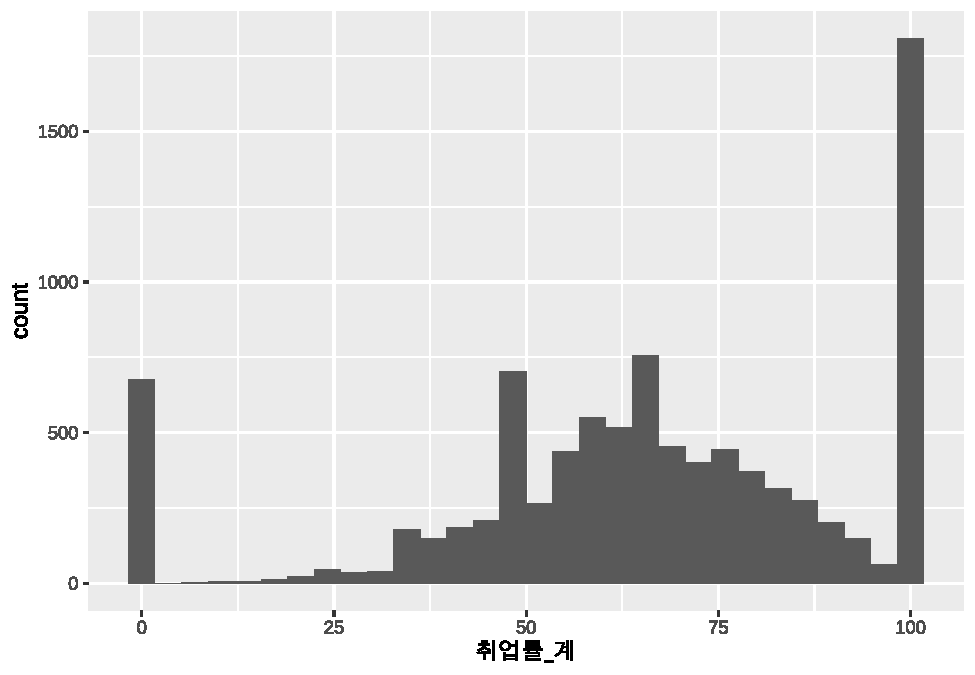
\includegraphics{chap3_files/figure-latex/unnamed-chunk-20-1.pdf}

\begin{Shaded}
\begin{Highlighting}[]
\DocumentationTok{\#\# p\_histogram에 x축을 \textquotesingle{}취업률\_계\textquotesingle{}열로 매핑, bins = 90으로 설정한 geom\_histogram 레이어를 생성 }
\NormalTok{p\_histogram }\SpecialCharTok{+}
  \FunctionTok{geom\_histogram}\NormalTok{(}\FunctionTok{aes}\NormalTok{(}\AttributeTok{x =}\NormalTok{ 취업률\_계), }\AttributeTok{bins =} \DecValTok{90}\NormalTok{)}
\end{Highlighting}
\end{Shaded}

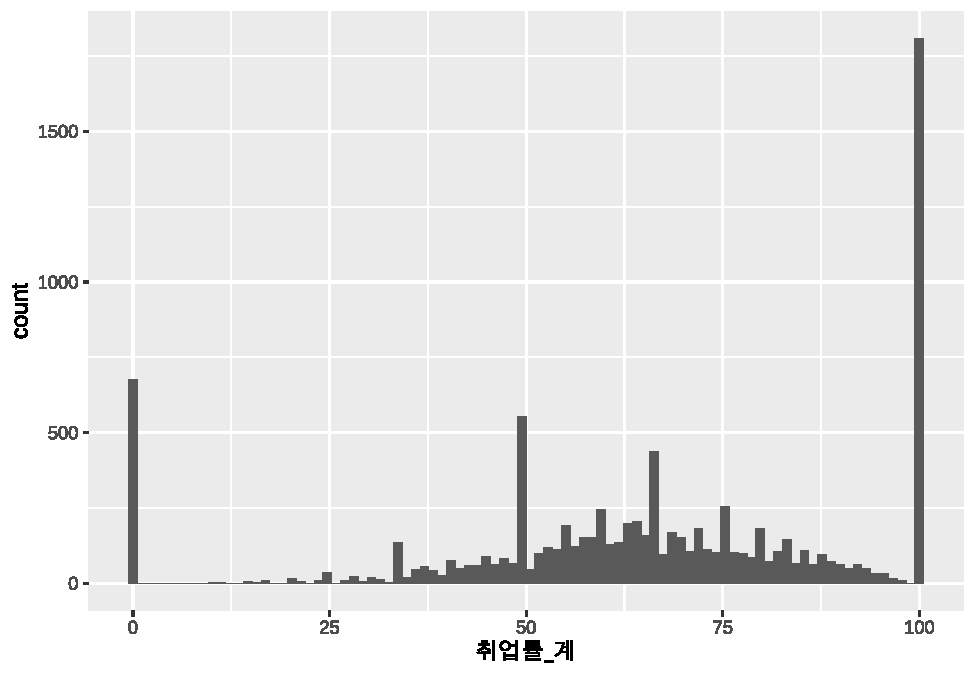
\includegraphics{chap3_files/figure-latex/unnamed-chunk-20-2.pdf}

\begin{Shaded}
\begin{Highlighting}[]
\DocumentationTok{\#\# p\_histogram에 x축을 \textquotesingle{}취업률\_계\textquotesingle{}열로 매핑, binwidth = 10으로 설정한 geom\_histogram 레이어를 생성 }
\NormalTok{p\_histogram }\SpecialCharTok{+}
  \FunctionTok{geom\_histogram}\NormalTok{(}\FunctionTok{aes}\NormalTok{(}\AttributeTok{x =}\NormalTok{ 취업률\_계), }\AttributeTok{binwidth =} \DecValTok{10}\NormalTok{)}
\end{Highlighting}
\end{Shaded}

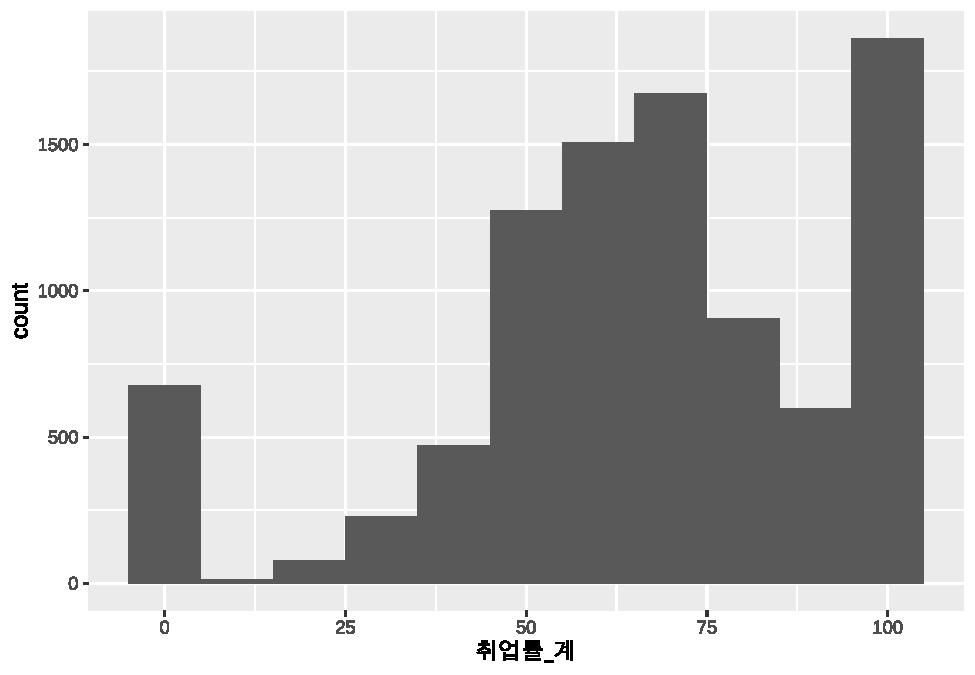
\includegraphics{chap3_files/figure-latex/unnamed-chunk-20-3.pdf}

\begin{Shaded}
\begin{Highlighting}[]
\DocumentationTok{\#\# p\_histogram에 x축을 \textquotesingle{}취업률\_계\textquotesingle{}열로 매핑, binwidth = 5으로 설정한 geom\_histogram 레이어를 생성 }
\NormalTok{p\_histogram }\SpecialCharTok{+}
  \FunctionTok{geom\_histogram}\NormalTok{(}\FunctionTok{aes}\NormalTok{(}\AttributeTok{x =}\NormalTok{ 취업률\_계), }\AttributeTok{binwidth =} \DecValTok{5}\NormalTok{)}
\end{Highlighting}
\end{Shaded}

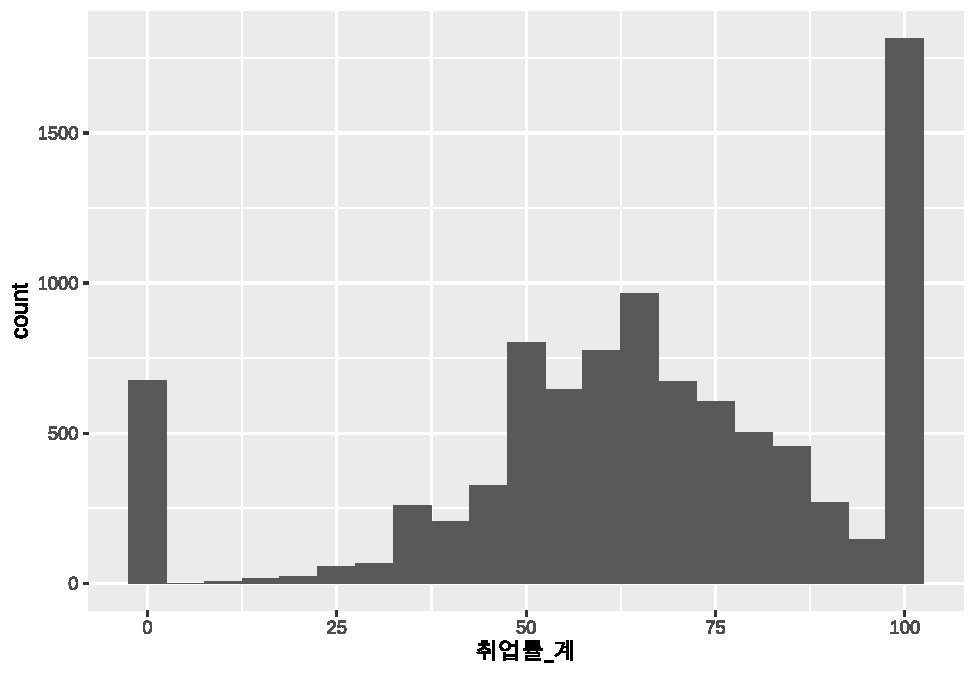
\includegraphics{chap3_files/figure-latex/unnamed-chunk-20-4.pdf}

\begin{Shaded}
\begin{Highlighting}[]
\DocumentationTok{\#\# p\_histogram에 x축을 \textquotesingle{}취업률\_계\textquotesingle{}열로 매핑, 각각의 미적요인을 설정한  geom\_histogram 레이어를 생성 }
\NormalTok{p\_histogram }\SpecialCharTok{+} 
  \FunctionTok{geom\_histogram}\NormalTok{(}\FunctionTok{aes}\NormalTok{(}\AttributeTok{x =}\NormalTok{ 취업률\_계), }\AttributeTok{color =} \StringTok{\textquotesingle{}red\textquotesingle{}}\NormalTok{, }\AttributeTok{fill =} \StringTok{\textquotesingle{}red\textquotesingle{}}\NormalTok{, }\AttributeTok{alpha =} \FloatTok{0.2}\NormalTok{, }\AttributeTok{linetype =} \DecValTok{2}\NormalTok{)}
\end{Highlighting}
\end{Shaded}

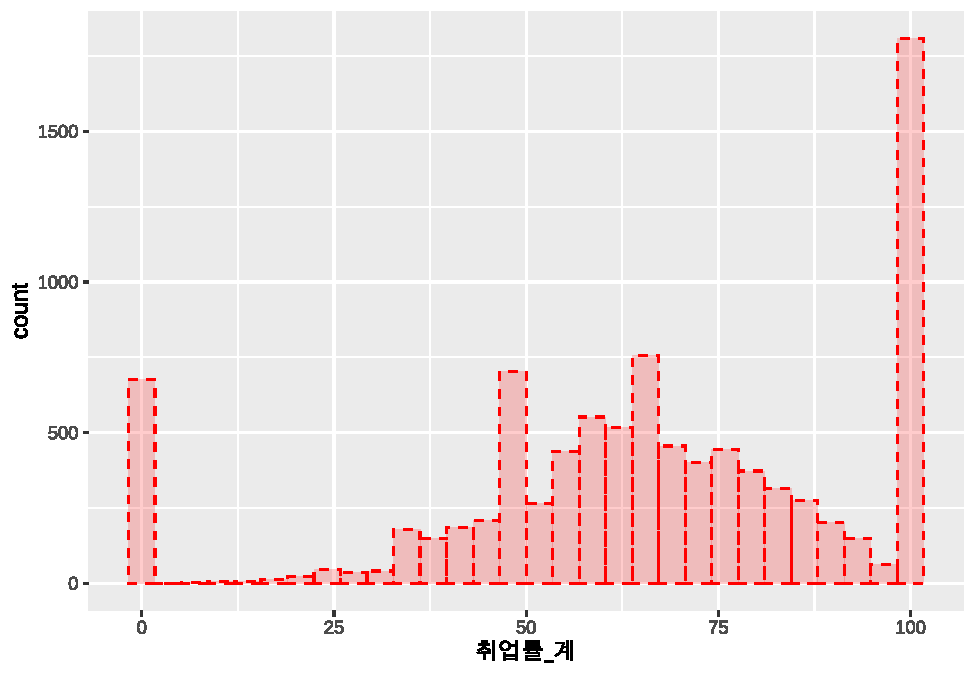
\includegraphics{chap3_files/figure-latex/unnamed-chunk-20-5.pdf}

2.3.1.1.2 \texttt{geom\_freqpoly()}

\texttt{geom\_freqpoly()} 는 하나의 데이터 열에 기록된 연속형 수치 데이터를 표현하는데 사용되는 기하요소 함수이다. 앞선 \texttt{geom\_histogram()} 은 막대를 사용하여 데이터의 수치를 표현해지만 \texttt{geom\_freqpoly()} 는 데이터 값들을 연결한 다각형을 사용하여 데이터의 수치를 표현한다.\texttt{geom\_freqpoly()}도 \texttt{geom\_histogram()}과 같이 binning을 기본적으로 사용하기 때문에 통계요소를 'bin'이 기본적으로 적용된다. 만약 다각형을 조금 부드럽게(smoothing) 하려면 통계요소를 'density'로 설정하는데 이 경우는 \texttt{geom\_density()}와 동일한 결과가 나온다.

\begin{Shaded}
\begin{Highlighting}[]
\FunctionTok{geom\_freqpoly}\NormalTok{(}\AttributeTok{mapping =} \ConstantTok{NULL}\NormalTok{, }\AttributeTok{data =} \ConstantTok{NULL}\NormalTok{,  }\AttributeTok{stat =} \StringTok{"bin"}\NormalTok{,  }\AttributeTok{position =} \StringTok{"identity"}\NormalTok{, }\AttributeTok{na.rm =} \ConstantTok{FALSE}\NormalTok{, }\AttributeTok{show.legend =} \ConstantTok{NA}\NormalTok{, ...)}
  \SpecialCharTok{{-}}\NormalTok{ mapping }\SpecialCharTok{:} \FunctionTok{aes}\NormalTok{()를 사용하여 매핑할 미적요소, 생략되면 }\FunctionTok{ggplot}\NormalTok{()에 정의된 미적매핑 사용}
  \SpecialCharTok{{-}}\NormalTok{ data }\SpecialCharTok{:}\NormalTok{ 시각화를 위해 사용될 데이터, 생략되면 }\FunctionTok{ggplot}\NormalTok{()에 정의된 데이터 사용}
  \SpecialCharTok{{-}}\NormalTok{ stat }\SpecialCharTok{:}\NormalTok{ 시각화에 적용될 통계요소, 기본값은 }\StringTok{\textquotesingle{}bin\textquotesingle{}}
  \SpecialCharTok{{-}}\NormalTok{ position }\SpecialCharTok{:}\NormalTok{ 시각화에 적용될 위치요소, 기본값은 }\StringTok{\textquotesingle{}identity\textquotesingle{}}
  \SpecialCharTok{{-}}\NormalTok{ na.rm }\SpecialCharTok{:} \ConstantTok{NA}\NormalTok{ 값을 생략할 것인지를 설정하는 논리값(}\ConstantTok{TRUE}\SpecialCharTok{/}\ConstantTok{FALSE}\NormalTok{)}
  \SpecialCharTok{{-}}\NormalTok{ show.legend }\SpecialCharTok{:}\NormalTok{ 범례를 사용할 것인지를 설정하는 논리값(}\ConstantTok{TRUE}\SpecialCharTok{/}\ConstantTok{FALSE}\NormalTok{)}
\end{Highlighting}
\end{Shaded}

\texttt{geom\_freqpoly()} 에서 사용이 가능한 미적요소는 위치(x, y), alpha, color, linetype, size, group이다.

\texttt{geom\_freqpoly()} 를 사용한 데이터 시각화는 다음과 같다.

\begin{Shaded}
\begin{Highlighting}[]
\DocumentationTok{\#\#  df\_취업통계를 ggplot 객체로 생성하고 p\_freqpoly에 저장}
\NormalTok{p\_freqpoly }\OtherTok{\textless{}{-}}\NormalTok{ df\_취업통계 }\SpecialCharTok{|}\ErrorTok{\textgreater{}}
  \FunctionTok{ggplot}\NormalTok{()}

\DocumentationTok{\#\# p\_freqpoly에 x축을 \textquotesingle{}취업률\_계\textquotesingle{}열로 매핑, bins = 30으로 설정한 geom\_freqpoly 레이어를 생성 }
\NormalTok{p\_freqpoly }\SpecialCharTok{+}
  \FunctionTok{geom\_freqpoly}\NormalTok{(}\FunctionTok{aes}\NormalTok{(}\AttributeTok{x =}\NormalTok{ 취업률\_계), }\AttributeTok{bins =} \DecValTok{30}\NormalTok{)}
\end{Highlighting}
\end{Shaded}

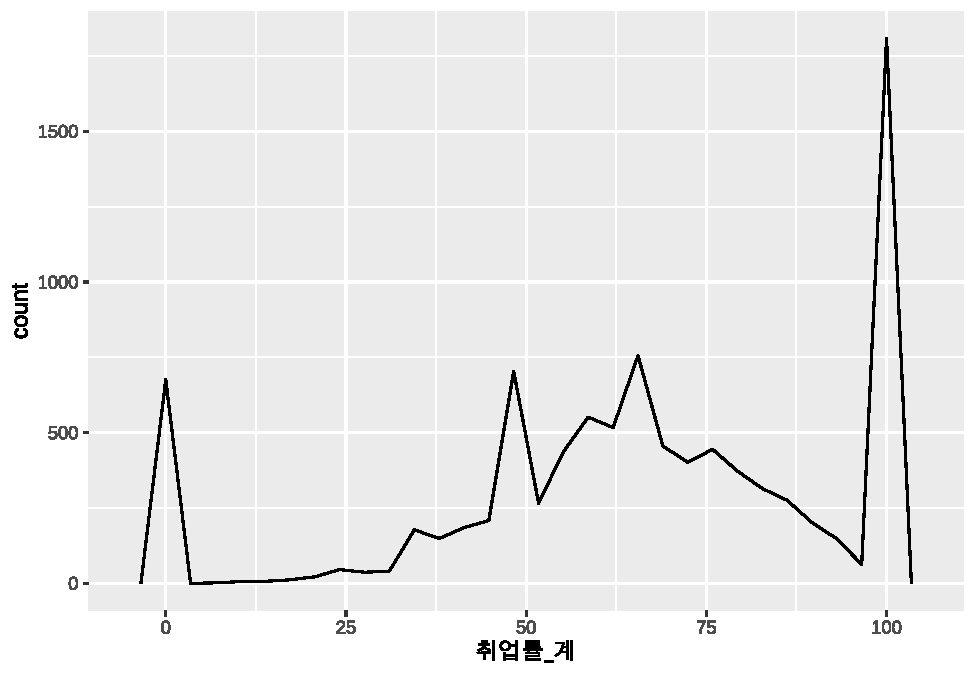
\includegraphics{chap3_files/figure-latex/unnamed-chunk-22-1.pdf}

\begin{Shaded}
\begin{Highlighting}[]
\DocumentationTok{\#\# p\_freqpoly에 x축을 \textquotesingle{}취업률\_계\textquotesingle{}열로 매핑, bins = 30으로 설정하는데 통계요소를 \textquotesingle{}density\textquotesingle{}로 설정한 geom\_freqpoly 레이어를 생성}
\NormalTok{p\_freqpoly }\SpecialCharTok{+}
  \FunctionTok{geom\_freqpoly}\NormalTok{(}\FunctionTok{aes}\NormalTok{(}\AttributeTok{x =}\NormalTok{ 취업률\_계), }\AttributeTok{stat =} \StringTok{\textquotesingle{}density\textquotesingle{}}\NormalTok{, }\AttributeTok{bins =} \DecValTok{30}\NormalTok{)}
\end{Highlighting}
\end{Shaded}

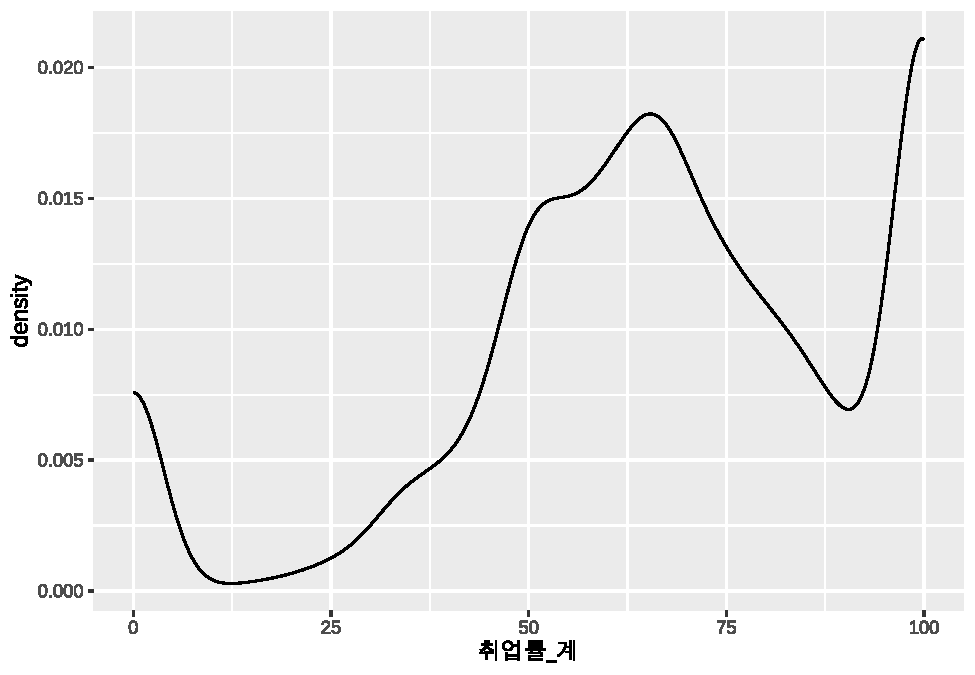
\includegraphics{chap3_files/figure-latex/unnamed-chunk-22-2.pdf}

\begin{Shaded}
\begin{Highlighting}[]
\DocumentationTok{\#\# p\_freqpoly에 x축을 \textquotesingle{}취업률\_계\textquotesingle{}열로 매핑, binwidth = 10으로 설정한 geom\_freqpoly 레이어를 생성 }
\NormalTok{p\_freqpoly }\SpecialCharTok{+}
  \FunctionTok{geom\_freqpoly}\NormalTok{(}\FunctionTok{aes}\NormalTok{(}\AttributeTok{x =}\NormalTok{ 취업률\_계), }\AttributeTok{binwidth =} \DecValTok{10}\NormalTok{, }\AttributeTok{rm.na =} \ConstantTok{TRUE}\NormalTok{)}
\end{Highlighting}
\end{Shaded}

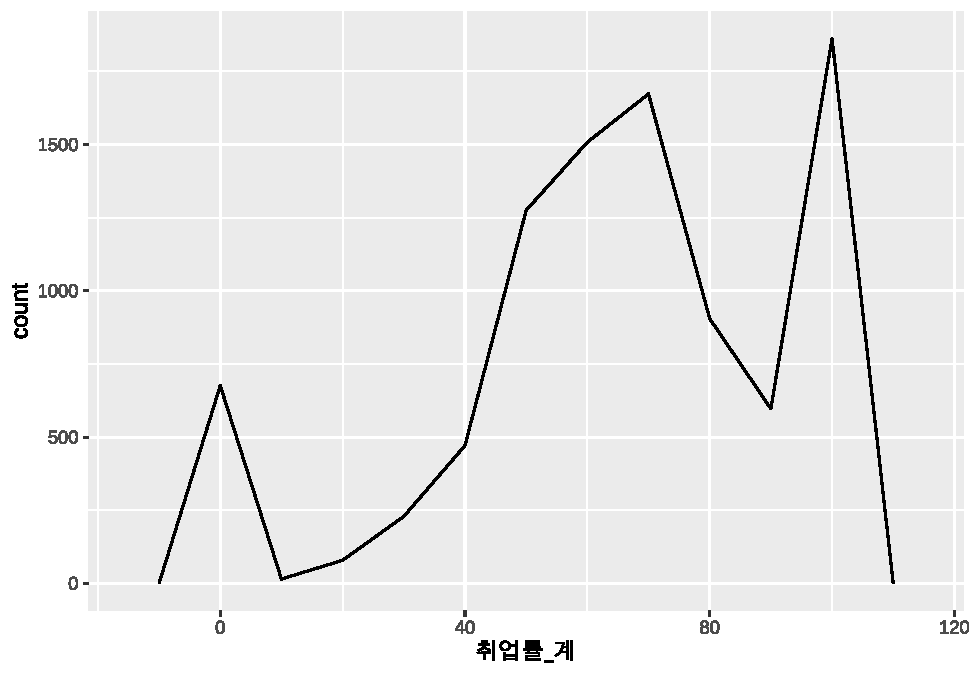
\includegraphics{chap3_files/figure-latex/unnamed-chunk-22-3.pdf}

\begin{Shaded}
\begin{Highlighting}[]
\DocumentationTok{\#\# p\_freqpoly에 x축을 \textquotesingle{}취업률\_계\textquotesingle{}열로 매핑, binwidth = 10으로 설정하고 미적요소를 설정한 geom\_freqpoly 레이어를 생성}
\NormalTok{p\_freqpoly }\SpecialCharTok{+}
  \FunctionTok{geom\_freqpoly}\NormalTok{(}\FunctionTok{aes}\NormalTok{(}\AttributeTok{x =}\NormalTok{ 취업률\_계), }\AttributeTok{binwidth =} \DecValTok{10}\NormalTok{, }\AttributeTok{color =} \StringTok{\textquotesingle{}red\textquotesingle{}}\NormalTok{, }\AttributeTok{linetype =} \DecValTok{2}\NormalTok{)}
\end{Highlighting}
\end{Shaded}

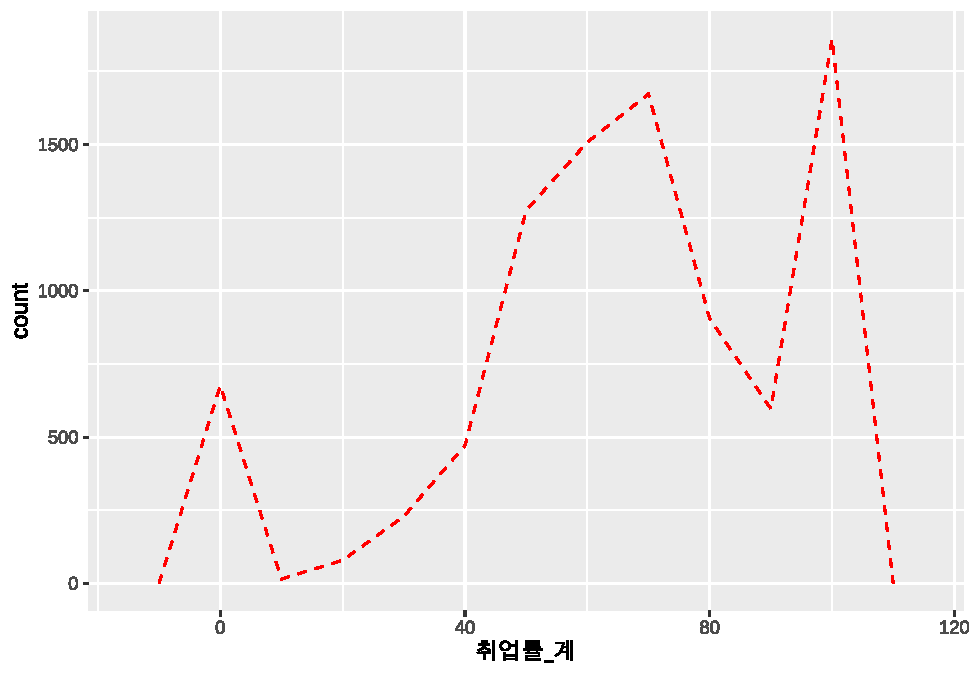
\includegraphics{chap3_files/figure-latex/unnamed-chunk-22-4.pdf}

\begin{Shaded}
\begin{Highlighting}[]
\DocumentationTok{\#\# p\_freqpoly에 x축을 \textquotesingle{}취업률\_계\textquotesingle{}열로 매핑, group과 color를 과정구분으로 매핑, binwidth = 10으로 설정한 geom\_freqpoly 레이어를 생성 }
\NormalTok{p\_freqpoly }\SpecialCharTok{+}
  \FunctionTok{geom\_freqpoly}\NormalTok{(}\FunctionTok{aes}\NormalTok{(}\AttributeTok{x =}\NormalTok{ 취업률\_계, }\AttributeTok{group =}\NormalTok{ 과정구분, }\AttributeTok{color =}\NormalTok{ 과정구분), }\AttributeTok{binwidth =} \DecValTok{10}\NormalTok{, }\AttributeTok{linetype =} \DecValTok{2}\NormalTok{)}
\end{Highlighting}
\end{Shaded}

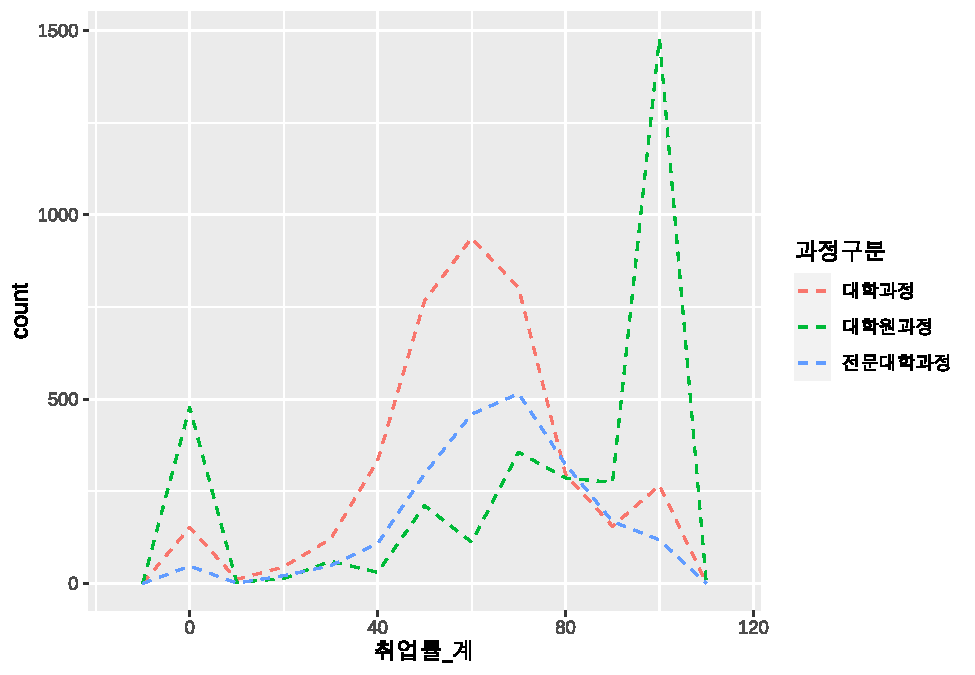
\includegraphics{chap3_files/figure-latex/unnamed-chunk-22-5.pdf}

2.3.1.1.3 \texttt{geom\_density()}

\texttt{geom\_density()} 도 하나의 데이터 열에 기록된 연속형 수치 데이터를 표현하는데 사용되는 기하요소 함수인데 데이터의 분포에 따른 확률분포함수를 표현하는 함수이다. 데이터 값으로 주어진 연속된 수치 데이터를 확률밀도함수에 대입하여 계산된 연속확률분포를 시각화한다. 따라서 X값에 따라 계산된 연속확률분포값은 확률값이기 때문에 1보다 작은 값들이고 이 값들이 연결되어 표현된다. \texttt{geom\_density()} 를 사용하여 연속확률분포를 시각화할 수 있다. 따라서 통계요소가 앞선 두 함수와는 달리 'density'가 기본값으로 설정된다.

\begin{Shaded}
\begin{Highlighting}[]
\FunctionTok{geom\_density}\NormalTok{(}\AttributeTok{mapping =} \ConstantTok{NULL}\NormalTok{, }\AttributeTok{data =} \ConstantTok{NULL}\NormalTok{, }\AttributeTok{stat =} \StringTok{"density"}\NormalTok{,  }\AttributeTok{position =} \StringTok{"identity"}\NormalTok{, }\AttributeTok{na.rm =} \ConstantTok{FALSE}\NormalTok{, }\AttributeTok{show.legend =} \ConstantTok{NA}\NormalTok{, ...)}
  \SpecialCharTok{{-}}\NormalTok{ mapping }\SpecialCharTok{:} \FunctionTok{aes}\NormalTok{()를 사용하여 매핑할 미적요소, 생략되면 }\FunctionTok{ggplot}\NormalTok{()에 정의된 미적매핑 사용}
  \SpecialCharTok{{-}}\NormalTok{ data }\SpecialCharTok{:}\NormalTok{ 시각화를 위해 사용될 데이터, 생략되면 }\FunctionTok{ggplot}\NormalTok{()에 정의된 데이터 사용}
  \SpecialCharTok{{-}}\NormalTok{ stat }\SpecialCharTok{:}\NormalTok{ 시각화에 적용될 통계요소, 기본값은 }\StringTok{\textquotesingle{}density\textquotesingle{}}
  \SpecialCharTok{{-}}\NormalTok{ position }\SpecialCharTok{:}\NormalTok{ 시각화에 적용될 위치요소, 기본값은 }\StringTok{\textquotesingle{}identity\textquotesingle{}}
  \SpecialCharTok{{-}}\NormalTok{ na.rm }\SpecialCharTok{:} \ConstantTok{NA}\NormalTok{ 값을 생략할 것인지를 설정하는 논리값(}\ConstantTok{TRUE}\SpecialCharTok{/}\ConstantTok{FALSE}\NormalTok{)}
  \SpecialCharTok{{-}}\NormalTok{ show.legend }\SpecialCharTok{:}\NormalTok{ 범례를 사용할 것인지를 설정하는 논리값(}\ConstantTok{TRUE}\SpecialCharTok{/}\ConstantTok{FALSE}\NormalTok{)}
\end{Highlighting}
\end{Shaded}

\texttt{geom\_density()} 에서 사용할 수 있는 미적요소는 위치(x, y), alpha, color, fill, linetype, size 등이다.

\begin{Shaded}
\begin{Highlighting}[]
\DocumentationTok{\#\#  df\_취업통계를 ggplot 객체로 생성하고 p\_density에 저장}
\NormalTok{p\_density }\OtherTok{\textless{}{-}}\NormalTok{ df\_취업통계 }\SpecialCharTok{|}\ErrorTok{\textgreater{}}
  \FunctionTok{ggplot}\NormalTok{()}

\DocumentationTok{\#\# p\_density객체에 x축을 \textquotesingle{}취업률\_계\textquotesingle{}열로 매핑한 geom\_density 레이어를 생성}
\NormalTok{p\_density }\SpecialCharTok{+} 
  \FunctionTok{geom\_density}\NormalTok{(}\FunctionTok{aes}\NormalTok{(}\AttributeTok{x =}\NormalTok{ 취업률\_계))}
\end{Highlighting}
\end{Shaded}

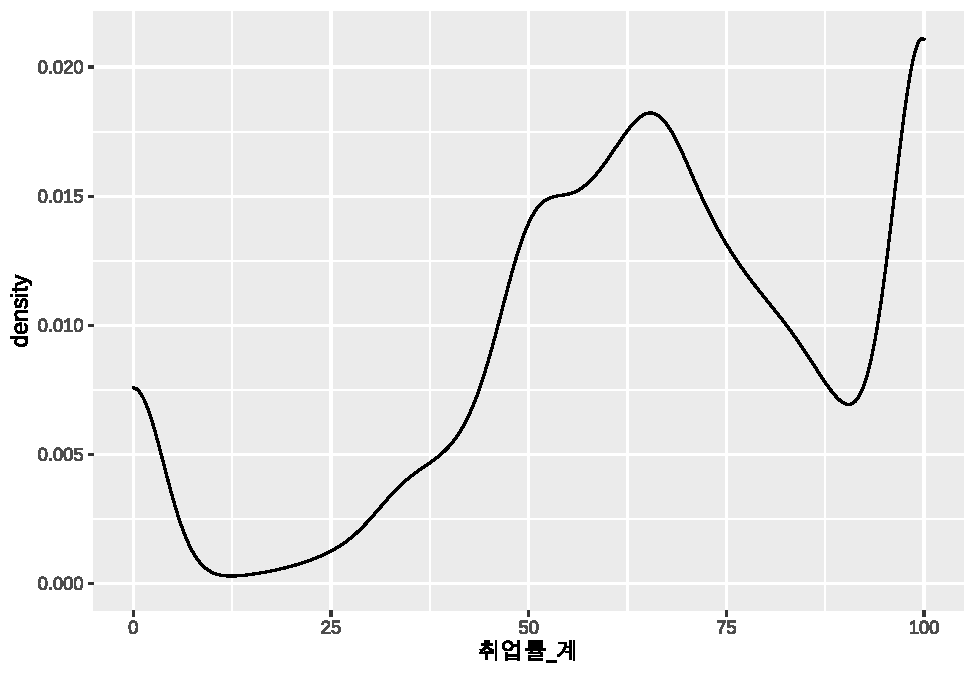
\includegraphics{chap3_files/figure-latex/unnamed-chunk-24-1.pdf}

\begin{Shaded}
\begin{Highlighting}[]
\DocumentationTok{\#\# p\_density객체에 x축을 \textquotesingle{}취업률\_계\textquotesingle{}열로 매핑, 미적요소 설정한 geom\_density 레이어를 생성}
\NormalTok{p\_density }\SpecialCharTok{+} 
  \FunctionTok{geom\_density}\NormalTok{(}\FunctionTok{aes}\NormalTok{(}\AttributeTok{x =}\NormalTok{ 취업률\_계), }\AttributeTok{color =} \StringTok{\textquotesingle{}blue\textquotesingle{}}\NormalTok{, }\AttributeTok{fill =} \StringTok{\textquotesingle{}skyblue\textquotesingle{}}\NormalTok{, }\AttributeTok{linetype =} \DecValTok{2}\NormalTok{, }\AttributeTok{size =} \DecValTok{1}\NormalTok{, }\AttributeTok{alpha =} \FloatTok{0.5}\NormalTok{)}
\end{Highlighting}
\end{Shaded}

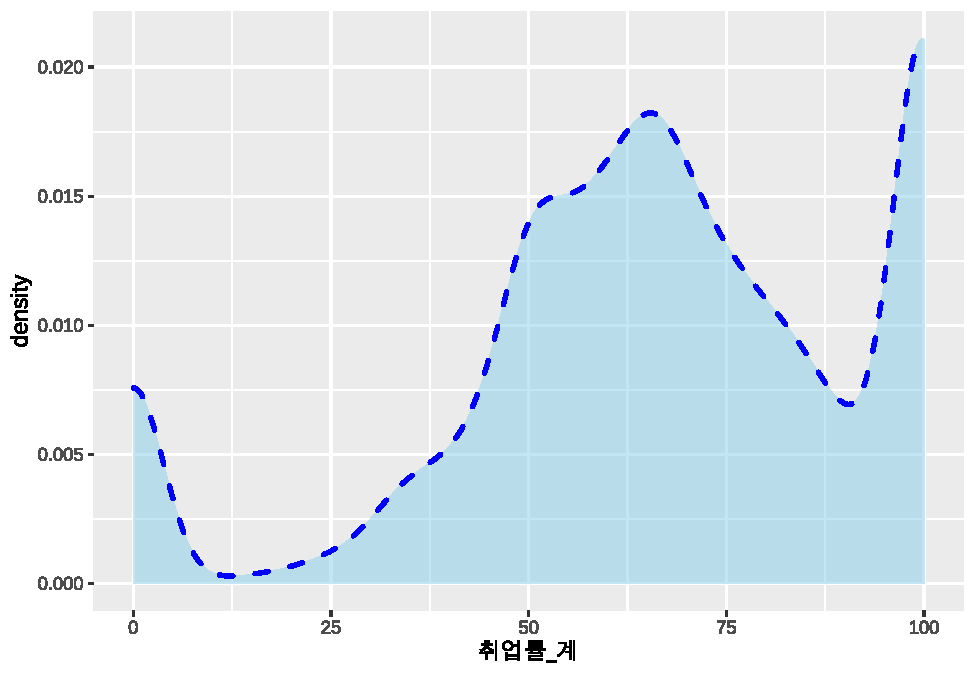
\includegraphics{chap3_files/figure-latex/unnamed-chunk-24-2.pdf}

\hypertarget{uxc774uxc0b0discrete-uxb370uxc774uxd130-geom_bar}{%
\subparagraph{\texorpdfstring{2.3.1.2 이산(Discrete) 데이터 : \texttt{geom\_bar()}}{2.3.1.2 이산(Discrete) 데이터 : geom\_bar()}}\label{uxc774uxc0b0discrete-uxb370uxc774uxd130-geom_bar}}

앞 절에서 설명한 \texttt{geom\_histogram()}, \texttt{geom\_freqpoly()}, \texttt{geom\_density()} 는 연속된 수치값에 대한 일변량 시각화 기하요소함수였다. 그렇다면 팩터와 같은 구분되고 분리되는 이산된 일변량 시각화는 어떻게 시각화되는가? 이산된 일변량 데이터를 위한 기하요소 함수는 \texttt{geom\_bar()} 가 유일하다. 사실 \texttt{geom\_bar()} 는 뒤에서 설명될 \texttt{geom\_col()} 과 거의 유사한 결과를 내는 막대 그래프 시각화이다. 다만 \texttt{geom\_bar()} 는 앞선 연속된 일변량 데이터 시각화와 같이 하나의 데이터만 제공되면 해당 데이터의 빈도를 자동적으로 계산하여 변수의 변량에 따른 데이터의 빈도를 막대 그래프 형태로 시각화한다. 이는 또 \texttt{geom\_histogram()} 과 유사하게 나타나지만 X축으로 제공되는 데이터가 연속형 수치 데이터인가 이산형 데이터인가에 따라 차이가 있다. 또 X 축에 매핑되는 데이터가 이산형 데이터이기 때문에 꼭 수치 데이터가 아닐 수 있다.

\begin{Shaded}
\begin{Highlighting}[]
\FunctionTok{geom\_bar}\NormalTok{(}\AttributeTok{mapping =} \ConstantTok{NULL}\NormalTok{, }\AttributeTok{data =} \ConstantTok{NULL}\NormalTok{, }\AttributeTok{stat =} \StringTok{"count"}\NormalTok{, }\AttributeTok{position =} \StringTok{"stack"}\NormalTok{, }\AttributeTok{width =} \ConstantTok{NULL}\NormalTok{, }\AttributeTok{na.rm =} \ConstantTok{FALSE}\NormalTok{, }\AttributeTok{show.legend =} \ConstantTok{NA}\NormalTok{, ...)}
  \SpecialCharTok{{-}}\NormalTok{ mapping }\SpecialCharTok{:} \FunctionTok{aes}\NormalTok{()를 사용하여 매핑할 미적요소, 생략되면 }\FunctionTok{ggplot}\NormalTok{()에 정의된 미적매핑 사용}
  \SpecialCharTok{{-}}\NormalTok{ data }\SpecialCharTok{:}\NormalTok{ 시각화를 위해 사용될 데이터, 생략되면 }\FunctionTok{ggplot}\NormalTok{()에 정의된 데이터 사용}
  \SpecialCharTok{{-}}\NormalTok{ stat }\SpecialCharTok{:}\NormalTok{ 시각화에 적용될 통계요소, 기본값은 }\StringTok{\textquotesingle{}count\textquotesingle{}}
  \SpecialCharTok{{-}}\NormalTok{ position }\SpecialCharTok{:}\NormalTok{ 시각화에 적용될 위치요소, 기본값은 }\StringTok{\textquotesingle{}stack\textquotesingle{}}
  \SpecialCharTok{{-}}\NormalTok{ na.rm }\SpecialCharTok{:} \ConstantTok{NA}\NormalTok{ 값을 생략할 것인지를 설정하는 논리값(}\ConstantTok{TRUE}\SpecialCharTok{/}\ConstantTok{FALSE}\NormalTok{)}
  \SpecialCharTok{{-}}\NormalTok{ show.legend }\SpecialCharTok{:}\NormalTok{ 범례를 사용할 것인지를 설정하는 논리값(}\ConstantTok{TRUE}\SpecialCharTok{/}\ConstantTok{FALSE}\NormalTok{) }
\end{Highlighting}
\end{Shaded}

\texttt{geom\_bar()} 에서 사용이 가능한 미적요소는 x, alpha, color, fill, linetype, size, weight가 있다.

\begin{Shaded}
\begin{Highlighting}[]
\DocumentationTok{\#\#  df\_취업통계를 ggplot 객체로 생성하고 p\_bar에 저장}
\NormalTok{p\_bar }\OtherTok{\textless{}{-}}\NormalTok{ df\_취업통계 }\SpecialCharTok{|}\ErrorTok{\textgreater{}}
  \FunctionTok{ggplot}\NormalTok{()}

\DocumentationTok{\#\# p\_bar 객체에 x축을 대계열로 매핑한 geom\_bar 레이어 생성 }
\NormalTok{p\_bar }\SpecialCharTok{+}
  \FunctionTok{geom\_bar}\NormalTok{(}\FunctionTok{aes}\NormalTok{(}\AttributeTok{x =}\NormalTok{ 대계열))}
\end{Highlighting}
\end{Shaded}

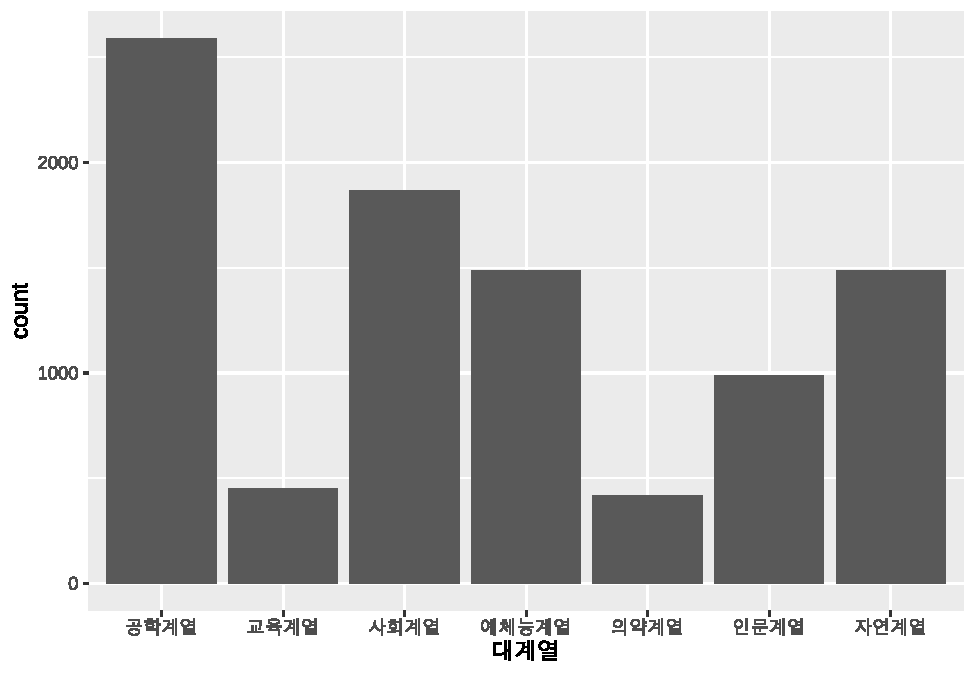
\includegraphics{chap3_files/figure-latex/unnamed-chunk-26-1.pdf}

\begin{Shaded}
\begin{Highlighting}[]
\DocumentationTok{\#\# p\_bar 객체에 x축을 대계열로 매핑하고 미적요소를 설정한 geom\_bar 레이어 생성}
\NormalTok{p\_bar }\SpecialCharTok{+}
  \FunctionTok{geom\_bar}\NormalTok{(}\FunctionTok{aes}\NormalTok{(}\AttributeTok{x =}\NormalTok{ 대계열), }\AttributeTok{color =} \StringTok{\textquotesingle{}blue\textquotesingle{}}\NormalTok{, }\AttributeTok{fill =} \StringTok{\textquotesingle{}skyblue\textquotesingle{}}\NormalTok{, }\AttributeTok{linetype =} \DecValTok{2}\NormalTok{, }\AttributeTok{size =} \DecValTok{1}\NormalTok{, }\AttributeTok{alpha =} \FloatTok{0.5}\NormalTok{)}
\end{Highlighting}
\end{Shaded}

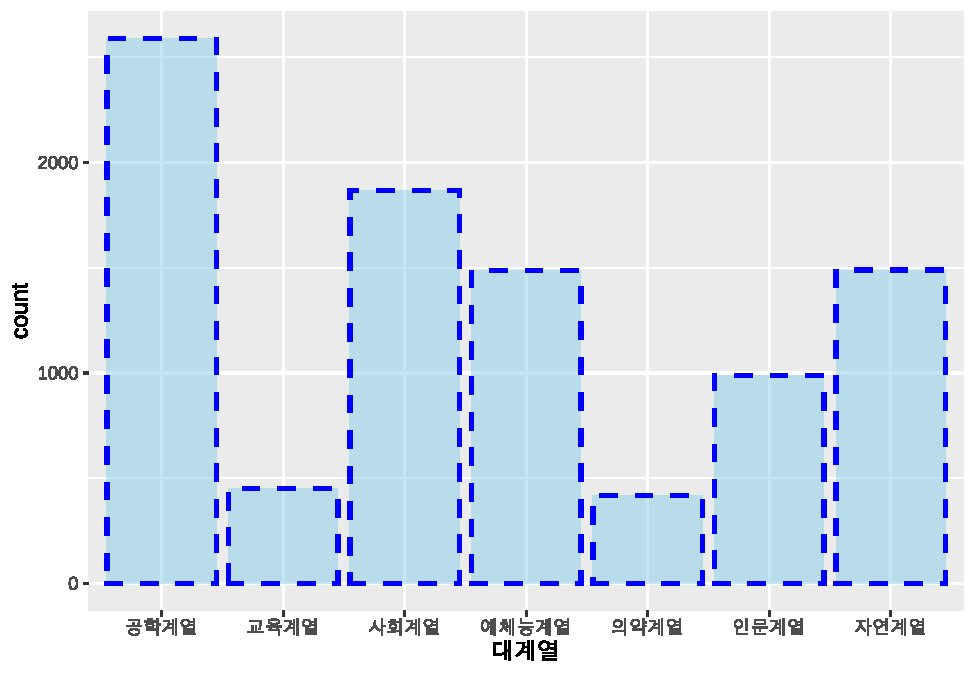
\includegraphics{chap3_files/figure-latex/unnamed-chunk-26-2.pdf}

\hypertarget{uxc774uxbcc0uxc218two-variable-uxb370uxc774uxd130-uxc2dcuxac01uxd654}{%
\paragraph{2.3.2 이변수(Two Variable) 데이터 시각화}\label{uxc774uxbcc0uxc218two-variable-uxb370uxc774uxd130-uxc2dcuxac01uxd654}}

앞서 언급한 바와 같이 \texttt{ggplot} 객체는 보통 X, Y 두 개의 축으로 표현되는 2차원 시각화를 기본으로 하고 있다. 따라서 변수 두개를 사용한 데이터 시각화가 일반적 형태의 시각화이다. 변수 두개를 사용한 데이터 시각화도 일변수 데이터 시각화와 마찬가지로 시각화해야할 데이터가 연속형 수치 데이터인지 이산형 데이터인지에 따라 사용하는 기하요소의 종류와 함수가 달라진다.

\hypertarget{uxac1cuxc758-uxc5f0uxc18duxd615-uxc218uxce58-uxbcc0uxc218}{%
\subparagraph{2.3.2.1 2개의 연속형 수치 변수}\label{uxac1cuxc758-uxc5f0uxc18duxd615-uxc218uxce58-uxbcc0uxc218}}

X축과 Y축에 매핑되어 시각화해야하는 두개의 변수가 모두 연속형 수치 변수인 경우에는 X축과 Y축의 매핑에 따라 위치를 표시해 주는 시각화가 대부분이다. 보통 데이터의 분포를 확인해야 하는 경우와 데이터에 수치값이나 텍스트를 표현해야 할 때 많이 사용된다.

2.3.2.1.1 \texttt{geom\_point()}

데이터의 전반적 분포를 확인할 때 가장 많이 사용되는 기하요소가 점을 사용한 데이터 시각화이다. 이렇게 X, Y축에 따라 데이터를 점으로 표현한 시각화를 산점도(Scatter Plot)라고 한다. 산점도는 X축과 Y축의 좌표값에 따라 점을 표시함으로서 데이터의 전반적인 분포를 살펴보고 X, Y축의 증감에 따른 데이터의 상관관계를 살펴보는데 효과적인 시각화 방법이다. 따라서 시각화 과정에서 데이터 값을 통계처리하지 않고 사용되기 때문에 통계요소가 'identity'로 설정된다.

\begin{Shaded}
\begin{Highlighting}[]
\FunctionTok{geom\_point}\NormalTok{(}\AttributeTok{mapping =} \ConstantTok{NULL}\NormalTok{, }\AttributeTok{data =} \ConstantTok{NULL}\NormalTok{,  }\AttributeTok{stat =} \StringTok{"identity"}\NormalTok{,  }\AttributeTok{position =} \StringTok{"identity"}\NormalTok{, }\AttributeTok{na.rm =} \ConstantTok{FALSE}\NormalTok{, }\AttributeTok{show.legend =} \ConstantTok{NA}\NormalTok{,  ...)}
  \SpecialCharTok{{-}}\NormalTok{ mapping }\SpecialCharTok{:} \FunctionTok{aes}\NormalTok{()를 사용하여 매핑할 미적요소, 생략되면 }\FunctionTok{ggplot}\NormalTok{()에 정의된 미적매핑 사용}
  \SpecialCharTok{{-}}\NormalTok{ data }\SpecialCharTok{:}\NormalTok{ 시각화를 위해 사용될 데이터, 생략되면 }\FunctionTok{ggplot}\NormalTok{()에 정의된 데이터 사용}
  \SpecialCharTok{{-}}\NormalTok{ stat }\SpecialCharTok{:}\NormalTok{ 시각화에 적용될 통계요소, 기본값은 }\StringTok{\textquotesingle{}identity\textquotesingle{}}
  \SpecialCharTok{{-}}\NormalTok{ position }\SpecialCharTok{:}\NormalTok{ 시각화에 적용될 위치요소, 기본값은 }\StringTok{\textquotesingle{}identity\textquotesingle{}}
  \SpecialCharTok{{-}}\NormalTok{ na.rm }\SpecialCharTok{:} \ConstantTok{NA}\NormalTok{ 값을 생략할 것인지를 설정하는 논리값(}\ConstantTok{TRUE}\SpecialCharTok{/}\ConstantTok{FALSE}\NormalTok{)}
  \SpecialCharTok{{-}}\NormalTok{ show.legend }\SpecialCharTok{:}\NormalTok{ 범례를 사용할 것인지를 설정하는 논리값(}\ConstantTok{TRUE}\SpecialCharTok{/}\ConstantTok{FALSE}\NormalTok{) }
\end{Highlighting}
\end{Shaded}

\texttt{geom\_point()}에서 사용이 가능한 미적요소는 x, y, alpha, colour, fill, group, shape, size, stroke 등이다.

\begin{Shaded}
\begin{Highlighting}[]
\DocumentationTok{\#\#  df\_취업통계 데이터 중 졸업자가 500명 이하인 학과를 필터링하여 ggplot 객체로 생성하고 p\_point에 저장}
\NormalTok{p\_point }\OtherTok{\textless{}{-}}\NormalTok{ df\_취업통계 }\SpecialCharTok{|}\ErrorTok{\textgreater{}} \FunctionTok{filter}\NormalTok{(졸업자\_계 }\SpecialCharTok{\textless{}} \DecValTok{500}\NormalTok{) }\SpecialCharTok{|}\ErrorTok{\textgreater{}}
  \FunctionTok{ggplot}\NormalTok{()}

\DocumentationTok{\#\#  p\_point객체에x축은 졸업자\_계, y축은 취업자\_합계\_계로 매핑한  geom\_point 레이어를 생성}
\NormalTok{p\_point }\SpecialCharTok{+}
  \FunctionTok{geom\_point}\NormalTok{(}\FunctionTok{aes}\NormalTok{(}\AttributeTok{x =}\NormalTok{ 졸업자\_계, }\AttributeTok{y =}\NormalTok{ 취업자\_합계\_계))}
\end{Highlighting}
\end{Shaded}

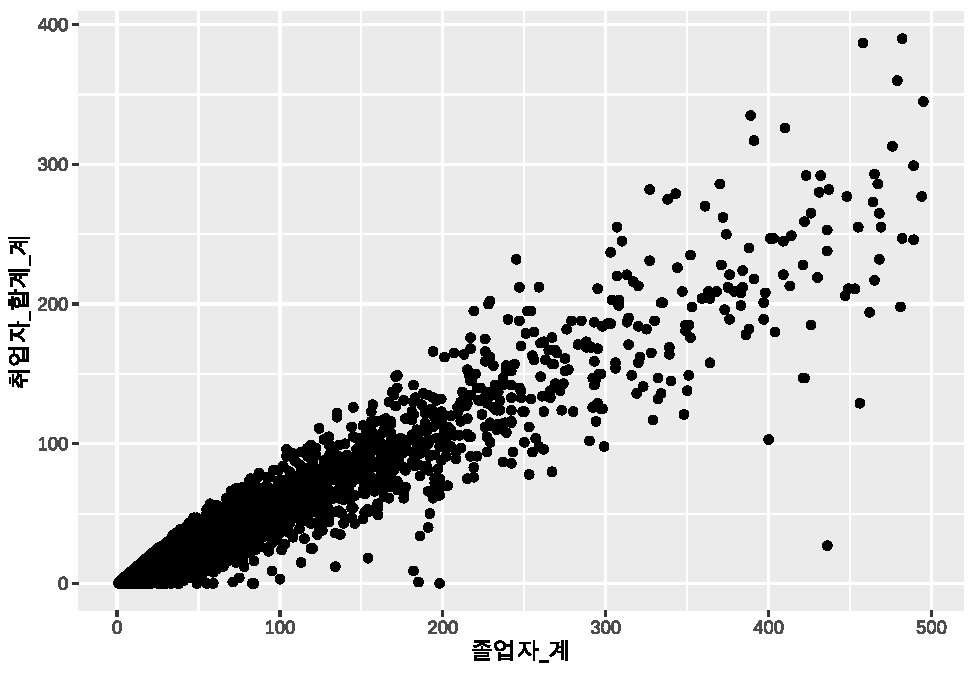
\includegraphics{chap3_files/figure-latex/unnamed-chunk-28-1.pdf}

\begin{Shaded}
\begin{Highlighting}[]
\DocumentationTok{\#\#  p\_point객체에 x축은 졸업자\_계, y축은 취업자\_합계\_계, color를 대계열로 매핑하고 투명도를 설정한 geom\_point 레이어를 생성}
\NormalTok{p\_point }\SpecialCharTok{+}
  \FunctionTok{geom\_point}\NormalTok{(}\FunctionTok{aes}\NormalTok{(}\AttributeTok{x =}\NormalTok{ 졸업자\_계, }\AttributeTok{y =}\NormalTok{ 취업자\_합계\_계, }\AttributeTok{color =}\NormalTok{ 대계열), }\AttributeTok{alpha =} \FloatTok{0.5}\NormalTok{)}
\end{Highlighting}
\end{Shaded}

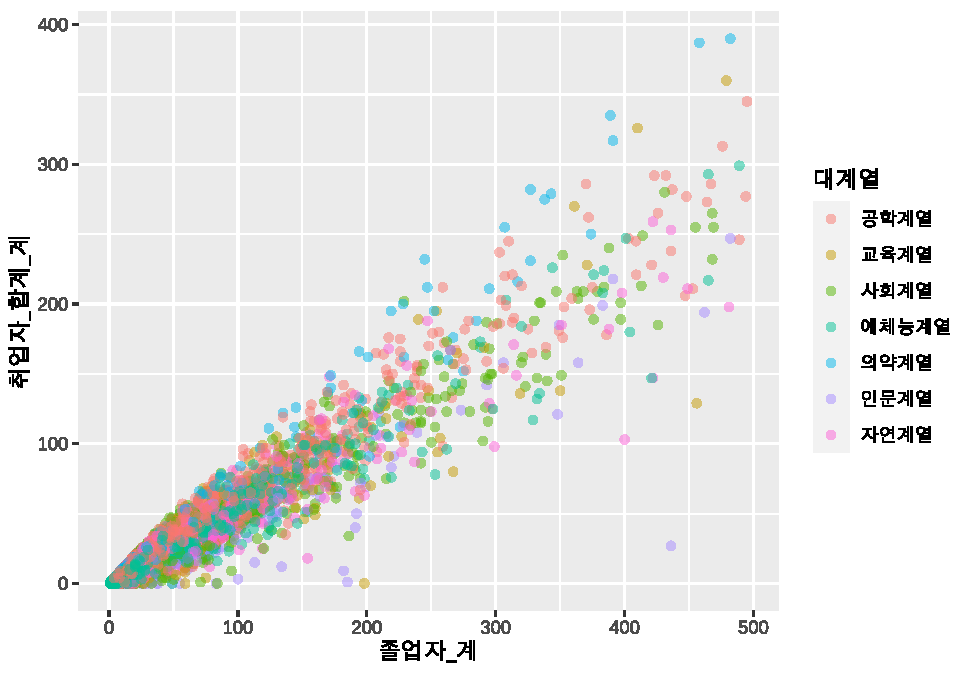
\includegraphics{chap3_files/figure-latex/unnamed-chunk-28-2.pdf}

2.3.2.1.2 \texttt{geom\_text()}

\texttt{geom\_text()}는 \texttt{geom\_point()}와 데이터 표현방식은 동일하나 표현되는 데이터가 문자열이라는 점에서 차이가 있다. \texttt{geom\_text()}는 주로 점이나 선, 막대 등으로 표현된 기하요소 레이어에 추가하여 해당 데이터들의 값이나 정보를 표현하기 위한 부가 정보를 제공하는데 활용된다. 그렇기 때문에 기본 기하요소와 겹쳐지 않기 위해 위치 조정을 위한 매개변수가 추가될 수 있다.

\begin{Shaded}
\begin{Highlighting}[]
\FunctionTok{geom\_text}\NormalTok{(}\AttributeTok{mapping =} \ConstantTok{NULL}\NormalTok{, }\AttributeTok{data =} \ConstantTok{NULL}\NormalTok{, }\AttributeTok{stat =} \StringTok{"identity"}\NormalTok{, }\AttributeTok{position =} \StringTok{"identity"}\NormalTok{, }\AttributeTok{nudge\_x =} \DecValTok{0}\NormalTok{, }\AttributeTok{nudge\_y =} \DecValTok{0}\NormalTok{, }\AttributeTok{check\_overlap =} \ConstantTok{FALSE}\NormalTok{, }\AttributeTok{na.rm =} \ConstantTok{FALSE}\NormalTok{, }\AttributeTok{show.legend =} \ConstantTok{NA}\NormalTok{, ...)}
  \SpecialCharTok{{-}}\NormalTok{ mapping }\SpecialCharTok{:} \FunctionTok{aes}\NormalTok{()를 사용하여 매핑할 미적요소, 생략되면 }\FunctionTok{ggplot}\NormalTok{()에 정의된 미적매핑 사용}
  \SpecialCharTok{{-}}\NormalTok{ data }\SpecialCharTok{:}\NormalTok{ 시각화를 위해 사용될 데이터, 생략되면 }\FunctionTok{ggplot}\NormalTok{()에 정의된 데이터 사용}
  \SpecialCharTok{{-}}\NormalTok{ stat }\SpecialCharTok{:}\NormalTok{ 시각화에 적용될 통계요소, 기본값은 }\StringTok{\textquotesingle{}identity\textquotesingle{}}
  \SpecialCharTok{{-}}\NormalTok{ position }\SpecialCharTok{:}\NormalTok{ 시각화에 적용될 위치요소, 기본값은 }\StringTok{\textquotesingle{}identity\textquotesingle{}}
  \SpecialCharTok{{-}}\NormalTok{ nudge\_x }\SpecialCharTok{:}\NormalTok{ X축 방향으로 문자열의 이동}
  \SpecialCharTok{{-}}\NormalTok{ nudge\_y }\SpecialCharTok{:}\NormalTok{  Y축 방향으로 문자열의 이동}
  \SpecialCharTok{{-}}\NormalTok{ check\_overlap }\SpecialCharTok{:}\NormalTok{ 텍스트가 겹치는 것을 허용할지에 대한 논리값(}\ConstantTok{TRUE}\SpecialCharTok{/}\ConstantTok{FALSE}\NormalTok{)}
  \SpecialCharTok{{-}}\NormalTok{ na.rm }\SpecialCharTok{:} \ConstantTok{NA}\NormalTok{ 값을 생략할 것인지를 설정하는 논리값(}\ConstantTok{TRUE}\SpecialCharTok{/}\ConstantTok{FALSE}\NormalTok{)}
  \SpecialCharTok{{-}}\NormalTok{ show.legend }\SpecialCharTok{:}\NormalTok{ 범례를 사용할 것인지를 설정하는 논리값(}\ConstantTok{TRUE}\SpecialCharTok{/}\ConstantTok{FALSE}\NormalTok{) }
\end{Highlighting}
\end{Shaded}

\texttt{geom\_text()}에서 사용 가능한 미적요소는 x, y, label, alpha, angle, color, family, fontface, group, hjust, lineheight, size, vjust 등이다.

\begin{itemize}
\item
  angle : 문자열이 표현되는 각도 설정
\item
  family : 문자열 시각화에 사용될 폰트 설정
\item
  fontface : 문자열 시각화에 사용될 문자 특성(``plain'', ``bold'', ``italic'', ``bold.italic'')
\item
  hjust : 수평 맞춤 설정, 0부터 1사이의 값을 지정
\item
  vjust : 수직 맞춤 설정, 0부터 1사이의 값을 지정
\item
  lineheight : 줄간격 설정, 0부터 1사이의 값을 지정
\end{itemize}

\begin{Shaded}
\begin{Highlighting}[]
\DocumentationTok{\#\#  df\_입학자 데이터 중 지역이 전체인 데이터를 필터링하여 ggplot 객체로 생성하고 p\_text에 저장}
\NormalTok{p\_text }\OtherTok{\textless{}{-}}\NormalTok{ df\_입학자 }\SpecialCharTok{|}\ErrorTok{\textgreater{}} \FunctionTok{filter}\NormalTok{(지역 }\SpecialCharTok{==} \StringTok{\textquotesingle{}전체\textquotesingle{}}\NormalTok{) }\SpecialCharTok{|}\ErrorTok{\textgreater{}}
  \FunctionTok{ggplot}\NormalTok{()}

\DocumentationTok{\#\#  p\_text에 x축은 연도, y축은 전문대학을 매핑한 geom\_point 레이어와 geom\_text레이어를 생성}
\NormalTok{p\_text }\SpecialCharTok{+}
  \FunctionTok{geom\_point}\NormalTok{(}\FunctionTok{aes}\NormalTok{(}\AttributeTok{x =}\NormalTok{ 연도, }\AttributeTok{y =}\NormalTok{ 전문대학)) }\SpecialCharTok{+}
  \FunctionTok{geom\_text}\NormalTok{(}\FunctionTok{aes}\NormalTok{(}\AttributeTok{x =}\NormalTok{ 연도, }\AttributeTok{y =}\NormalTok{ 전문대학, }\AttributeTok{label =}\NormalTok{ 전문대학))}
\end{Highlighting}
\end{Shaded}

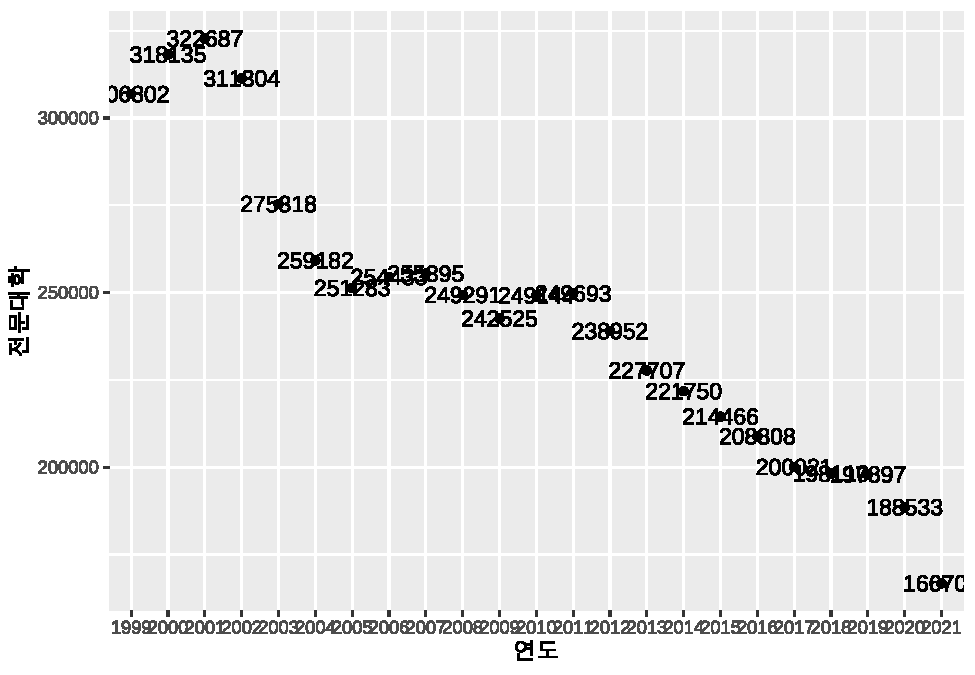
\includegraphics{chap3_files/figure-latex/unnamed-chunk-30-1.pdf}

\begin{Shaded}
\begin{Highlighting}[]
\DocumentationTok{\#\#  p\_text에 x축은 연도, y축은 전문대학을 매핑하고 미적요소를 설정한 geom\_point 레이어와 geom\_text레이어를 생성}
\NormalTok{p\_text }\SpecialCharTok{+}
  \FunctionTok{geom\_point}\NormalTok{(}\FunctionTok{aes}\NormalTok{(}\AttributeTok{x =}\NormalTok{ 연도, }\AttributeTok{y =}\NormalTok{ 전문대학)) }\SpecialCharTok{+}
  \FunctionTok{geom\_text}\NormalTok{(}\FunctionTok{aes}\NormalTok{(}\AttributeTok{x =}\NormalTok{ 연도, }\AttributeTok{y =}\NormalTok{ 전문대학, }\AttributeTok{label =}\NormalTok{ 전문대학), }\AttributeTok{nudge\_x =} \DecValTok{1}\NormalTok{, }\AttributeTok{fontface =} \StringTok{\textquotesingle{}bold\textquotesingle{}}\NormalTok{)}
\end{Highlighting}
\end{Shaded}

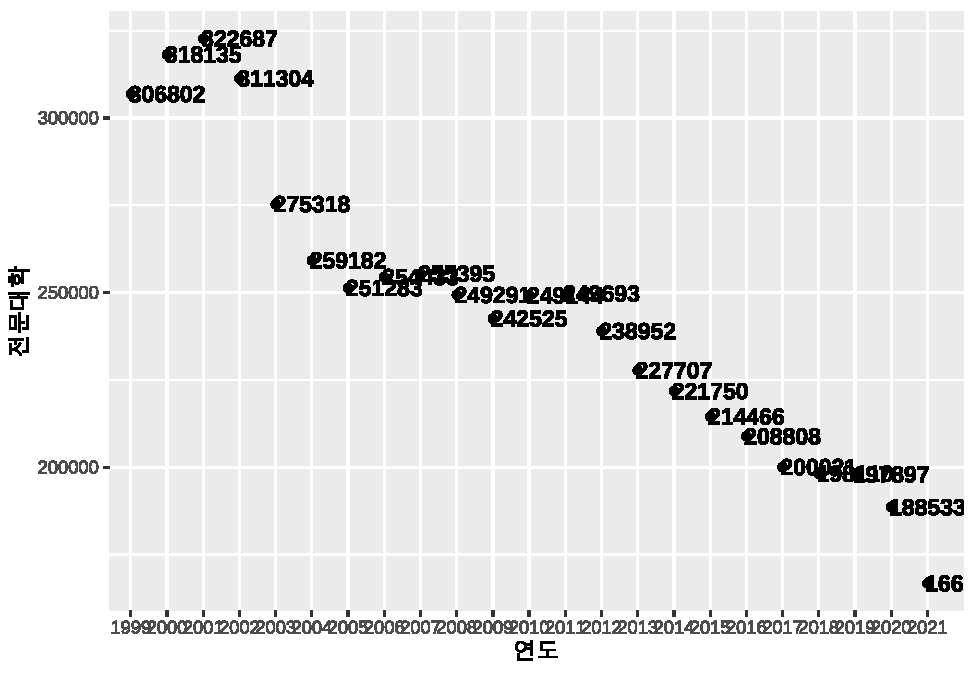
\includegraphics{chap3_files/figure-latex/unnamed-chunk-30-2.pdf}

2.3.2.1.3 \texttt{geom\_label()}

\texttt{geom\_label()}은 \texttt{geom\_text()}와 거의 유사한 시각화를 제공한다. 다만 \texttt{geom\_text()}는 문자열만을 시각화하지만 \texttt{geom\_label()}은 박스로 둘러싸여진 문자열을 시각화한다. 따라서 문자열을 둘러싸고 있는 박스에 대한 설정외에는 \texttt{geom\_text()}의 설정과 동일하다.

\begin{Shaded}
\begin{Highlighting}[]
\FunctionTok{geom\_label}\NormalTok{(}\AttributeTok{mapping =} \ConstantTok{NULL}\NormalTok{, }\AttributeTok{data =} \ConstantTok{NULL}\NormalTok{, }\AttributeTok{stat =} \StringTok{"identity"}\NormalTok{, }\AttributeTok{position =} \StringTok{"identity"}\NormalTok{, }\AttributeTok{nudge\_x =} \DecValTok{0}\NormalTok{, }\AttributeTok{nudge\_y =} \DecValTok{0}\NormalTok{, }\AttributeTok{label.padding =} \FunctionTok{unit}\NormalTok{(}\FloatTok{0.25}\NormalTok{, }\StringTok{"lines"}\NormalTok{), }\AttributeTok{label.r =} \FunctionTok{unit}\NormalTok{(}\FloatTok{0.15}\NormalTok{, }\StringTok{"lines"}\NormalTok{), }\AttributeTok{label.size =} \FloatTok{0.25}\NormalTok{, }\AttributeTok{na.rm =} \ConstantTok{FALSE}\NormalTok{, }\AttributeTok{show.legend =} \ConstantTok{NA}\NormalTok{, ...)}
  \SpecialCharTok{{-}}\NormalTok{ mapping }\SpecialCharTok{:} \FunctionTok{aes}\NormalTok{()를 사용하여 매핑할 미적요소, 생략되면 }\FunctionTok{ggplot}\NormalTok{()에 정의된 미적매핑 사용}
  \SpecialCharTok{{-}}\NormalTok{ data }\SpecialCharTok{:}\NormalTok{ 시각화를 위해 사용될 데이터, 생략되면 }\FunctionTok{ggplot}\NormalTok{()에 정의된 데이터 사용}
  \SpecialCharTok{{-}}\NormalTok{ stat }\SpecialCharTok{:}\NormalTok{ 시각화에 적용될 통계요소, 기본값은 }\StringTok{\textquotesingle{}identity\textquotesingle{}}
  \SpecialCharTok{{-}}\NormalTok{ position }\SpecialCharTok{:}\NormalTok{ 시각화에 적용될 위치요소, 기본값은 }\StringTok{\textquotesingle{}identity\textquotesingle{}}
  \SpecialCharTok{{-}}\NormalTok{ nudge\_x }\SpecialCharTok{:}\NormalTok{ X축 방향으로 문자열의 이동}
  \SpecialCharTok{{-}}\NormalTok{ nudge\_y }\SpecialCharTok{:}\NormalTok{  Y축 방향으로 문자열의 이동}
  \SpecialCharTok{{-}}\NormalTok{ label.padding }\SpecialCharTok{:}\NormalTok{ 박스와 문자열간의 여백 설정}
  \SpecialCharTok{{-}}\NormalTok{ label.r }\OtherTok{=}\NormalTok{ 박스의 귀퉁이를 둥글게 설정할 경우 반지름 설정}
  \SpecialCharTok{{-}}\NormalTok{ label.size }\OtherTok{=}\NormalTok{ 박스 라인의 두께 설정}
  \SpecialCharTok{{-}}\NormalTok{ na.rm }\SpecialCharTok{:} \ConstantTok{NA}\NormalTok{ 값을 생략할 것인지를 설정하는 논리값(}\ConstantTok{TRUE}\SpecialCharTok{/}\ConstantTok{FALSE}\NormalTok{)}
  \SpecialCharTok{{-}}\NormalTok{ show.legend }\SpecialCharTok{:}\NormalTok{ 범례를 사용할 것인지를 설정하는 논리값(}\ConstantTok{TRUE}\SpecialCharTok{/}\ConstantTok{FALSE}\NormalTok{) }
\end{Highlighting}
\end{Shaded}

\texttt{geom\_label()}에서 사용 가능한 미적요소는 x, y, label, alpha, angle, color, family, fontface, group, hjust, lineheight, size, vjust 등이다.

\begin{Shaded}
\begin{Highlighting}[]
\DocumentationTok{\#\#  df\_입학자 데이터 중 지역이 전체인 데이터를 필터링하여 ggplot 객체로 생성하고 p\_label에 저장}
\NormalTok{p\_label }\OtherTok{\textless{}{-}}\NormalTok{ df\_입학자 }\SpecialCharTok{|}\ErrorTok{\textgreater{}} \FunctionTok{filter}\NormalTok{(지역 }\SpecialCharTok{==} \StringTok{\textquotesingle{}전체\textquotesingle{}}\NormalTok{) }\SpecialCharTok{|}\ErrorTok{\textgreater{}}
  \FunctionTok{ggplot}\NormalTok{()}

\DocumentationTok{\#\#  p\_label에 x축은 연도, y축은 전문대학을 매핑 geom\_point 레이어와 geom\_label 레이어를 생성}
\NormalTok{p\_label }\SpecialCharTok{+}
  \FunctionTok{geom\_point}\NormalTok{(}\FunctionTok{aes}\NormalTok{(}\AttributeTok{x =}\NormalTok{ 연도, }\AttributeTok{y =}\NormalTok{ 전문대학)) }\SpecialCharTok{+}
  \FunctionTok{geom\_label}\NormalTok{(}\FunctionTok{aes}\NormalTok{(}\AttributeTok{x =}\NormalTok{ 연도, }\AttributeTok{y =}\NormalTok{ 전문대학, }\AttributeTok{label =}\NormalTok{ 전문대학))}
\end{Highlighting}
\end{Shaded}

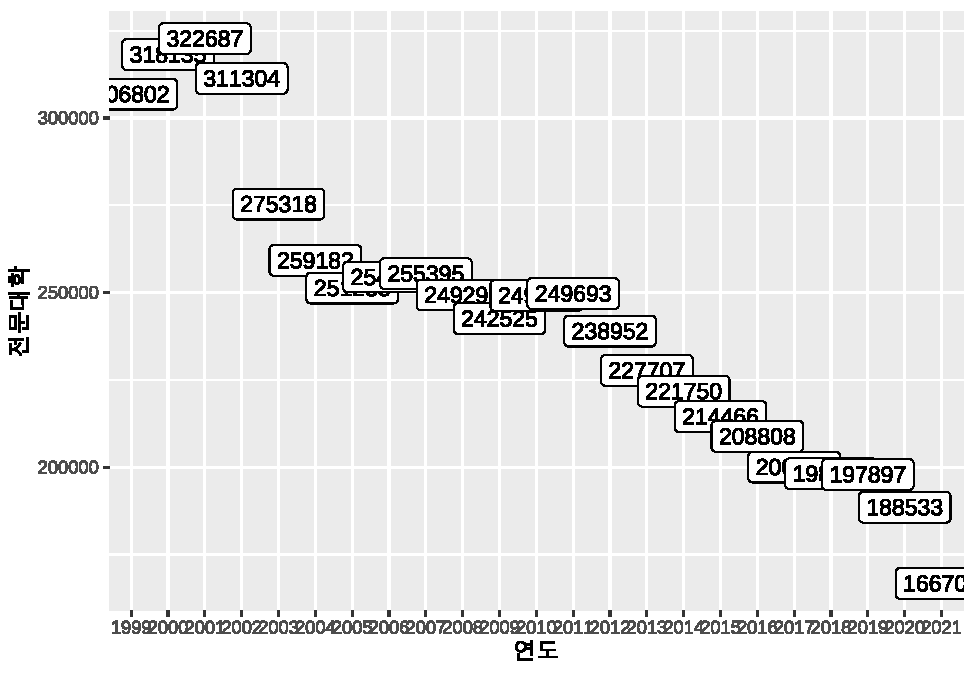
\includegraphics{chap3_files/figure-latex/unnamed-chunk-32-1.pdf}

\begin{Shaded}
\begin{Highlighting}[]
\DocumentationTok{\#\#  p\_label에 x축은 연도, y축은 전문대학을 매핑하고 미적요소를 설정한 geom\_point 레이어와 geom\_label 레이어를 생성}
\NormalTok{p\_label }\SpecialCharTok{+}
  \FunctionTok{geom\_point}\NormalTok{(}\FunctionTok{aes}\NormalTok{(}\AttributeTok{x =}\NormalTok{ 연도, }\AttributeTok{y =}\NormalTok{ 전문대학)) }\SpecialCharTok{+}
  \FunctionTok{geom\_label}\NormalTok{(}\FunctionTok{aes}\NormalTok{(}\AttributeTok{x =}\NormalTok{ 연도, }\AttributeTok{y =}\NormalTok{ 전문대학, }\AttributeTok{label =}\NormalTok{ 전문대학), }\AttributeTok{nudge\_x =} \DecValTok{1}\NormalTok{, }\AttributeTok{fontface =} \StringTok{\textquotesingle{}bold\textquotesingle{}}\NormalTok{)}
\end{Highlighting}
\end{Shaded}

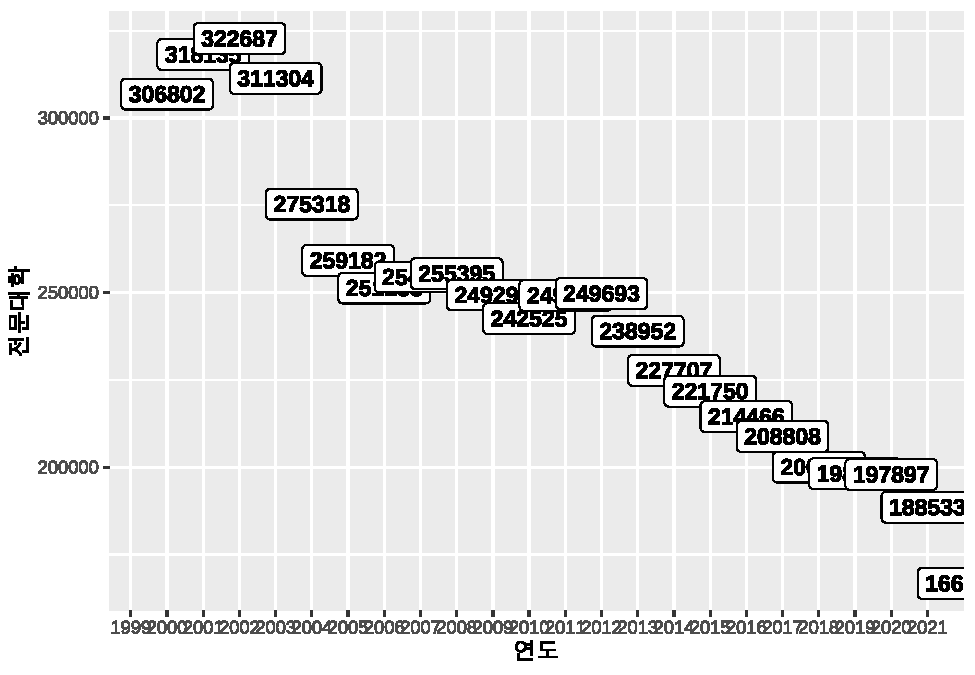
\includegraphics{chap3_files/figure-latex/unnamed-chunk-32-2.pdf}

2.3.2.1.4 \texttt{geom\_smooth()}

\texttt{geom\_smooth()}는 데이터의 전반적인 추세선을 표현하는 기하요소 함수이다. 이 추세선은 데이터의 패턴을 찾기 위해 사용되고 특히 오버플로팅된 데이터에 대한 패턴을 찾아낼때 유용하게 사용된다. \texttt{geom\_smooth()}에서 추세선을 결정하기 위해 제공하는 통계 방법은 ``lm'', ``glm'', ``gam'', ``loess''의 네가지를 제공한다.

\begin{Shaded}
\begin{Highlighting}[]
\FunctionTok{geom\_smooth}\NormalTok{(}\AttributeTok{mapping =} \ConstantTok{NULL}\NormalTok{, }\AttributeTok{data =} \ConstantTok{NULL}\NormalTok{, }\AttributeTok{stat =} \StringTok{"smooth"}\NormalTok{, }\AttributeTok{position =} \StringTok{"identity"}\NormalTok{, }\AttributeTok{method =} \ConstantTok{NULL}\NormalTok{,   }\AttributeTok{formula =} \ConstantTok{NULL}\NormalTok{, }\AttributeTok{se =} \ConstantTok{TRUE}\NormalTok{, }\AttributeTok{na.rm =} \ConstantTok{FALSE}\NormalTok{, }\AttributeTok{orientation =} \ConstantTok{NA}\NormalTok{, }\AttributeTok{show.legend =} \ConstantTok{NA}\NormalTok{, ...)}
  \SpecialCharTok{{-}}\NormalTok{ mapping }\SpecialCharTok{:} \FunctionTok{aes}\NormalTok{()를 사용하여 매핑할 미적요소, 생략되면 }\FunctionTok{ggplot}\NormalTok{()에 정의된 미적매핑 사용}
  \SpecialCharTok{{-}}\NormalTok{ data }\SpecialCharTok{:}\NormalTok{ 시각화를 위해 사용될 데이터, 생략되면 }\FunctionTok{ggplot}\NormalTok{()에 정의된 데이터 사용}
  \SpecialCharTok{{-}}\NormalTok{ stat }\SpecialCharTok{:}\NormalTok{ 시각화에 적용될 통계요소, 기본값은 }\StringTok{\textquotesingle{}smooth\textquotesingle{}}
  \SpecialCharTok{{-}}\NormalTok{ position }\SpecialCharTok{:}\NormalTok{ 시각화에 적용될 위치요소, 기본값은 }\StringTok{\textquotesingle{}identity\textquotesingle{}}
  \SpecialCharTok{{-}}\NormalTok{ method }\SpecialCharTok{:}\NormalTok{ 추세선을 결정하기 위해 사용하는 통계 방법 설정, }\StringTok{"lm"}\NormalTok{, }\StringTok{"glm"}\NormalTok{, }\StringTok{"gam"}\NormalTok{, }\StringTok{"loess"}\NormalTok{ 중 하나임}
  \SpecialCharTok{{-}}\NormalTok{ formula }\SpecialCharTok{:}\NormalTok{  추세선을 결정하기 위해 사용하는 함수식 설정}
  \SpecialCharTok{{-}}\NormalTok{ se }\SpecialCharTok{:}\NormalTok{ 추세선에 대한 표준오차 설정을 위한 논리값(}\ConstantTok{TRUE}\SpecialCharTok{/}\ConstantTok{FALSE}\NormalTok{)}
  \SpecialCharTok{{-}}\NormalTok{ na.rm }\SpecialCharTok{:} \ConstantTok{NA}\NormalTok{ 값을 생략할 것인지를 설정하는 논리값(}\ConstantTok{TRUE}\SpecialCharTok{/}\ConstantTok{FALSE}\NormalTok{)}
  \SpecialCharTok{{-}}\NormalTok{ show.legend }\SpecialCharTok{:}\NormalTok{ 범례를 사용할 것인지를 설정하는 논리값(}\ConstantTok{TRUE}\SpecialCharTok{/}\ConstantTok{FALSE}\NormalTok{) }
\end{Highlighting}
\end{Shaded}

\texttt{geom\_smooth()}에서 사용 가능한 미적요소는 x, y, alpha, color, fill, group, linetype, size, weight, ymax, ymin 등이다.

\begin{Shaded}
\begin{Highlighting}[]
\DocumentationTok{\#\#  df\_입학자 데이터 중 지역이 전체인 데이터를 필터링하여 ggplot 객체로 생성하고 p\_smooth에 저장}
\NormalTok{p\_smooth }\OtherTok{\textless{}{-}}\NormalTok{ df\_입학자 }\SpecialCharTok{|}\ErrorTok{\textgreater{}} \FunctionTok{filter}\NormalTok{(지역 }\SpecialCharTok{==} \StringTok{\textquotesingle{}전체\textquotesingle{}}\NormalTok{) }\SpecialCharTok{|}\ErrorTok{\textgreater{}}
  \FunctionTok{ggplot}\NormalTok{()}

\DocumentationTok{\#\#  p\_smooth에 x축은 연도, y축은 전문대학을 매핑, geom\_smooth의 추세선 결정 방법은 \textquotesingle{}loess\textquotesingle{}로 설정한 geom\_line레이어와 geom\_smooth레이어를 생성}
\NormalTok{p\_smooth }\SpecialCharTok{+}
  \FunctionTok{geom\_line}\NormalTok{(}\FunctionTok{aes}\NormalTok{(}\AttributeTok{x =}\NormalTok{ 연도, }\AttributeTok{y =}\NormalTok{ 전문대학, }\AttributeTok{group =} \DecValTok{1}\NormalTok{)) }\SpecialCharTok{+}
  \FunctionTok{geom\_smooth}\NormalTok{(}\FunctionTok{aes}\NormalTok{(}\AttributeTok{x =}\NormalTok{ 연도, }\AttributeTok{y =}\NormalTok{ 전문대학, }\AttributeTok{group =} \DecValTok{1}\NormalTok{), }\AttributeTok{method =} \StringTok{\textquotesingle{}loess\textquotesingle{}}\NormalTok{)}
\end{Highlighting}
\end{Shaded}

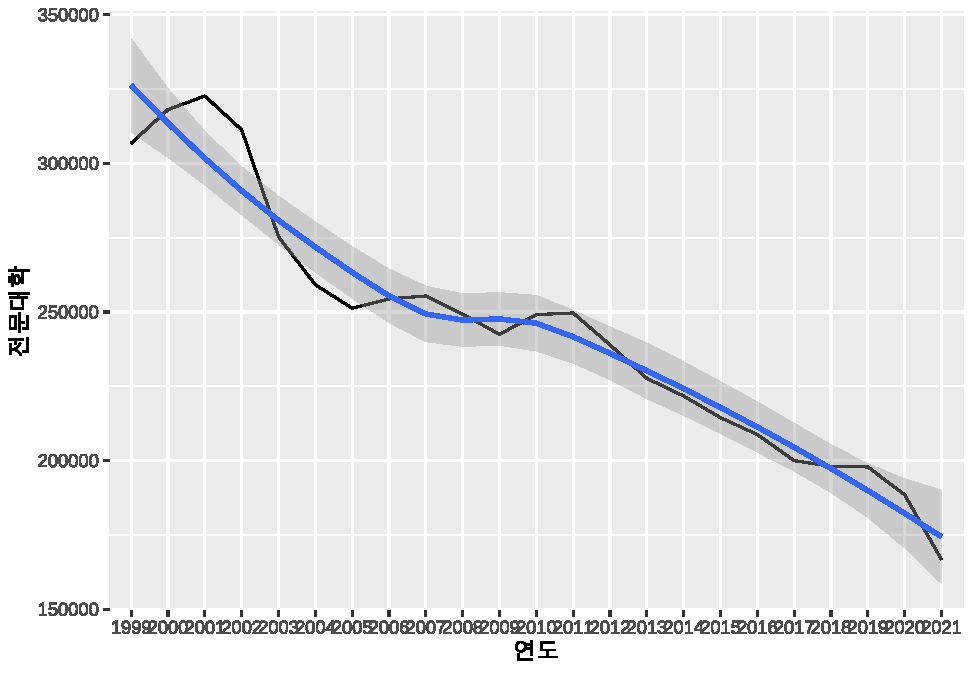
\includegraphics{chap3_files/figure-latex/unnamed-chunk-34-1.pdf}

\begin{Shaded}
\begin{Highlighting}[]
\DocumentationTok{\#\#  p\_smooth에 x축은 연도, y축은 전문대학을 매핑, geom\_smooth의 추세선 결정 방법은 \textquotesingle{}lm\textquotesingle{}, se는 FALSE로 설정한 geom\_line레이어와 geom\_smooth레이어를 생성}
\NormalTok{p\_smooth }\SpecialCharTok{+}
  \FunctionTok{geom\_line}\NormalTok{(}\FunctionTok{aes}\NormalTok{(}\AttributeTok{x =}\NormalTok{ 연도, }\AttributeTok{y =}\NormalTok{ 전문대학, }\AttributeTok{group =} \DecValTok{1}\NormalTok{)) }\SpecialCharTok{+}
  \FunctionTok{geom\_smooth}\NormalTok{(}\FunctionTok{aes}\NormalTok{(}\AttributeTok{x =}\NormalTok{ 연도, }\AttributeTok{y =}\NormalTok{ 전문대학, }\AttributeTok{group =} \DecValTok{1}\NormalTok{), }\AttributeTok{method =} \StringTok{\textquotesingle{}lm\textquotesingle{}}\NormalTok{, }\AttributeTok{se =} \ConstantTok{FALSE}\NormalTok{)}
\end{Highlighting}
\end{Shaded}

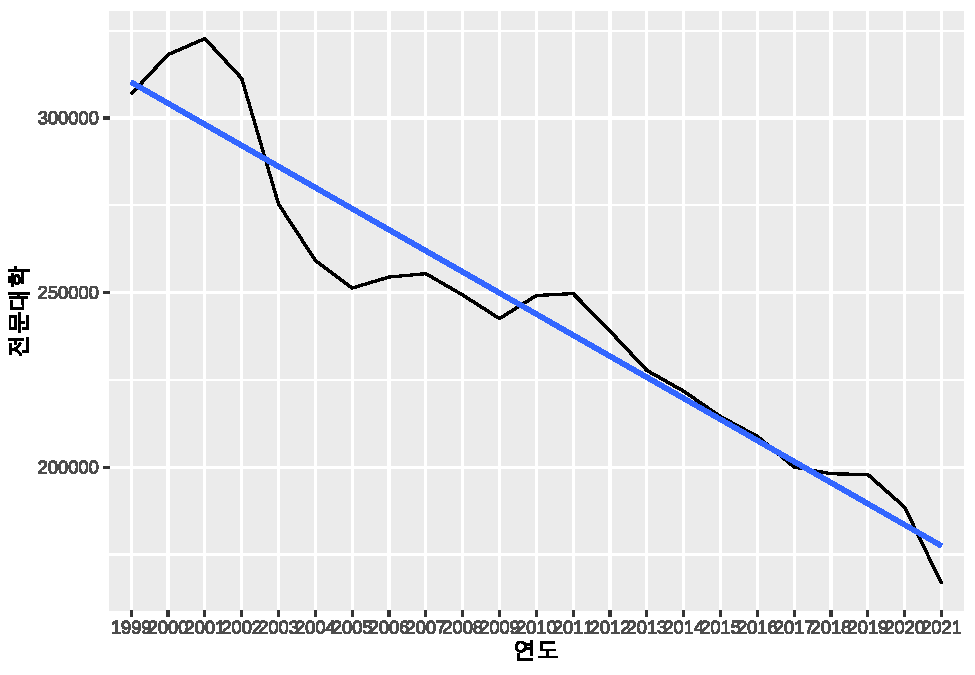
\includegraphics{chap3_files/figure-latex/unnamed-chunk-34-2.pdf}

\hypertarget{uxc5f0uxc18duxd615-uxc218uxce58-uxbcc0uxc218uxc640-uxc774uxc0b0uxd615-uxbcc0uxc218}{%
\subparagraph{2.3.2.2 연속형 수치 변수와 이산형 변수}\label{uxc5f0uxc18duxd615-uxc218uxce58-uxbcc0uxc218uxc640-uxc774uxc0b0uxd615-uxbcc0uxc218}}

반별 성적 평균이라던지 지역별 매출액 평균등을 시각화 할 때같이 연속형 수치변수와 이산형 변수를 사용하여 데이터를 시각화하는 경우가 많이 있다. 사실 시각화의 가장 효과적인 활용 방법이 이 경우일 것이다.

2.3.2.2.1 \texttt{geom\_col()}

\texttt{geom\_col()}은 막대그래프를 그리기 위해 사용하는 시각화 함수이다. 앞에서 막대그래프는 이미 \texttt{geom\_histogram()}과 \texttt{geom\_bar()}가 설명되었다. 그런데 또 \texttt{geom\_col()}이 제공된다. 막대그래프는 시각화하고자 하는 데이터의 종류에 따라 각각의 특성에 맞는 함수가 제공된다. 하지만 \texttt{geom\_col()}이 가장 포괄적인 막대그래프 시각화 함수로써 \texttt{geom\_col()}를 사용하여 \texttt{geom\_histogram()}과 \texttt{geom\_bar()}와 동일한 막대그래프를 그릴 수도 있다. 특히 \texttt{geom\_col()}은 \texttt{geom\_bar(stat\ =\ \textquotesingle{}ideneity)}와 동일한 시각화 효과를 낸다.

\begin{Shaded}
\begin{Highlighting}[]
\FunctionTok{geom\_col}\NormalTok{(}\AttributeTok{mapping =} \ConstantTok{NULL}\NormalTok{, }\AttributeTok{data =} \ConstantTok{NULL}\NormalTok{, }\AttributeTok{position =} \StringTok{"stack"}\NormalTok{, }\AttributeTok{width =} \ConstantTok{NULL}\NormalTok{, }\AttributeTok{na.rm =} \ConstantTok{FALSE}\NormalTok{, }\AttributeTok{show.legend =} \ConstantTok{NA}\NormalTok{, ...)}
  \SpecialCharTok{{-}}\NormalTok{ mapping }\SpecialCharTok{:} \FunctionTok{aes}\NormalTok{()를 사용하여 매핑할 미적요소, 생략되면 }\FunctionTok{ggplot}\NormalTok{()에 정의된 미적매핑 사용}
  \SpecialCharTok{{-}}\NormalTok{ data }\SpecialCharTok{:}\NormalTok{ 시각화를 위해 사용될 데이터, 생략되면 }\FunctionTok{ggplot}\NormalTok{()에 정의된 데이터 사용}
  \SpecialCharTok{{-}}\NormalTok{ position }\SpecialCharTok{:}\NormalTok{ 시각화에 적용될 위치요소, 기본값은 }\StringTok{\textquotesingle{}stack\textquotesingle{}}
  \SpecialCharTok{{-}}\NormalTok{ width }\SpecialCharTok{:}\NormalTok{ 막대의 너비 설정}
  \SpecialCharTok{{-}}\NormalTok{ na.rm }\SpecialCharTok{:} \ConstantTok{NA}\NormalTok{ 값을 생략할 것인지를 설정하는 논리값(}\ConstantTok{TRUE}\SpecialCharTok{/}\ConstantTok{FALSE}\NormalTok{)}
  \SpecialCharTok{{-}}\NormalTok{ show.legend }\SpecialCharTok{:}\NormalTok{ 범례를 사용할 것인지를 설정하는 논리값(}\ConstantTok{TRUE}\SpecialCharTok{/}\ConstantTok{FALSE}\NormalTok{) }
\end{Highlighting}
\end{Shaded}

\texttt{geom\_col()}에서 특별하게 활용되는 매개변수가 \texttt{position}이다. 이 \texttt{position}를 설정하여 막대그래프의 타입을 달리하여 시각화가 가능하다는 것이다. \texttt{position}의 종류는 다음 절에서 자세히 설명하도록 하겠다. \texttt{geom\_col()}에서 사용 가능한 미적요소는 x, y, alpha, color, fill, group, linetype, size 등이다.

\begin{Shaded}
\begin{Highlighting}[]
\DocumentationTok{\#\#  df\_입학자 데이터 중 지역이 전체가 아닌 데이터를 필터링하여 ggplot 객체로 생성하고 p\_col에 저장}
\NormalTok{p\_col }\OtherTok{\textless{}{-}}\NormalTok{ df\_입학자 }\SpecialCharTok{|}\ErrorTok{\textgreater{}} \FunctionTok{filter}\NormalTok{(지역 }\SpecialCharTok{!=} \StringTok{\textquotesingle{}전체\textquotesingle{}}\NormalTok{) }\SpecialCharTok{|}\ErrorTok{\textgreater{}}
  \FunctionTok{ggplot}\NormalTok{()}

\DocumentationTok{\#\#  p\_col에 x축은 연도, y축은 일반대학을 매핑한 geom\_col레이어를 생성}
\NormalTok{p\_col }\SpecialCharTok{+}
  \FunctionTok{geom\_col}\NormalTok{(}\FunctionTok{aes}\NormalTok{(}\AttributeTok{x =}\NormalTok{ 연도, }\AttributeTok{y =}\NormalTok{ 일반대학))}
\end{Highlighting}
\end{Shaded}

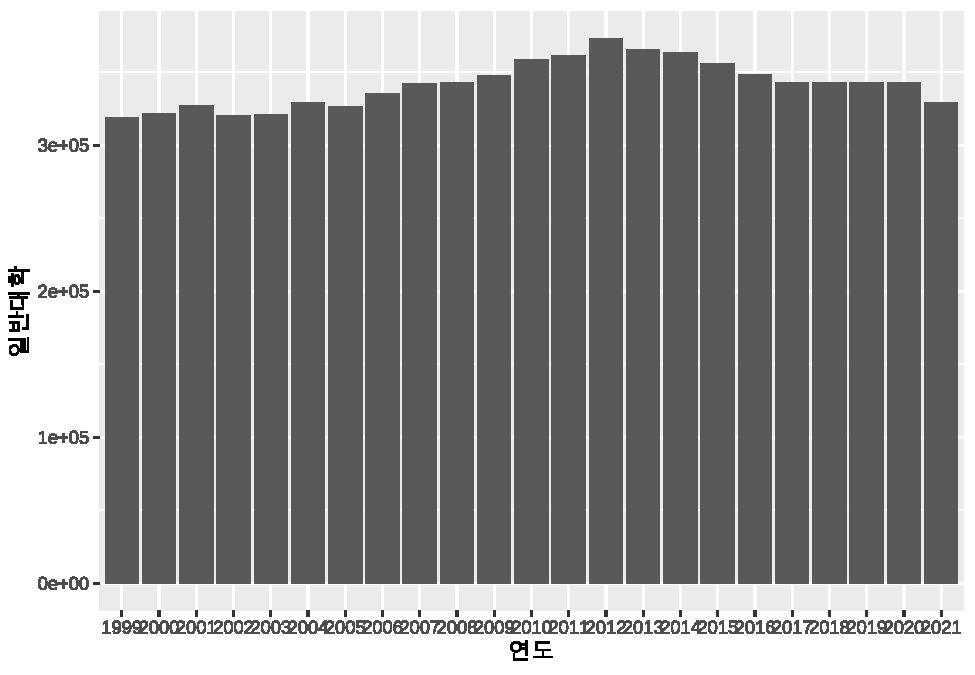
\includegraphics{chap3_files/figure-latex/unnamed-chunk-36-1.pdf}

\begin{Shaded}
\begin{Highlighting}[]
\DocumentationTok{\#\#  p\_col에 x축은 연도, y축은 일반대학을 매핑하고 stat을 \textquotesingle{}identity\textquotesingle{}로 설정한 geom\_col레이어를 생성}
\NormalTok{p\_col }\SpecialCharTok{+}
  \FunctionTok{geom\_bar}\NormalTok{(}\FunctionTok{aes}\NormalTok{(}\AttributeTok{x =}\NormalTok{ 연도, }\AttributeTok{y =}\NormalTok{ 일반대학), }\AttributeTok{stat =} \StringTok{\textquotesingle{}identity\textquotesingle{}}\NormalTok{)}
\end{Highlighting}
\end{Shaded}

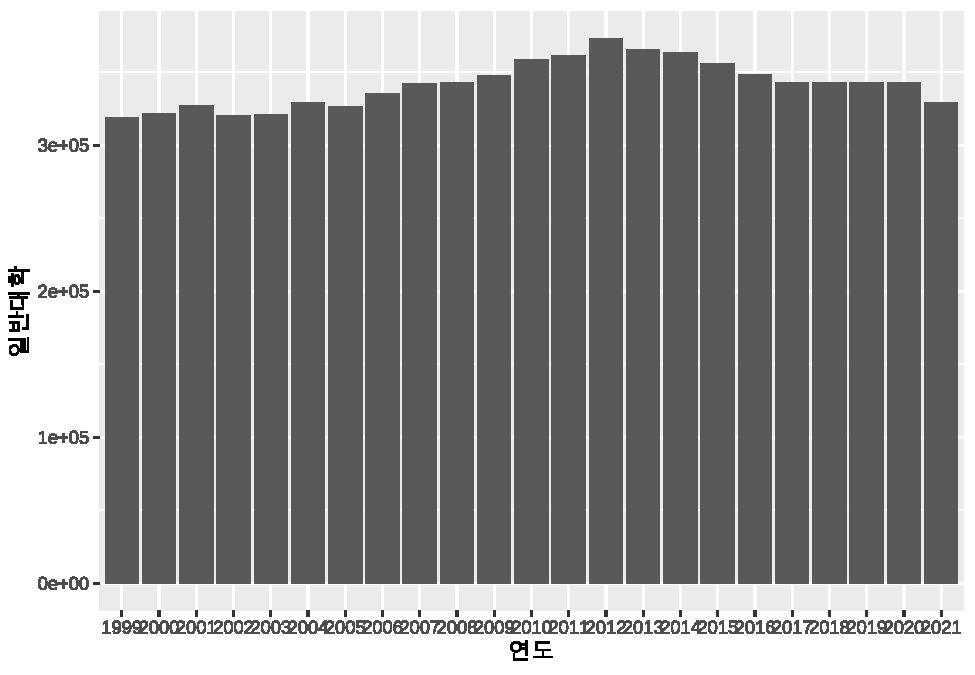
\includegraphics{chap3_files/figure-latex/unnamed-chunk-36-2.pdf}

\begin{Shaded}
\begin{Highlighting}[]
\DocumentationTok{\#\#  p\_col에 x축은 연도, y축은 일반대학, fill을 지역으로 매핑한 geom\_col레이어를 생성}
\NormalTok{p\_col }\SpecialCharTok{+}
  \FunctionTok{geom\_col}\NormalTok{(}\FunctionTok{aes}\NormalTok{(}\AttributeTok{x =}\NormalTok{ 연도, }\AttributeTok{y =}\NormalTok{ 일반대학, }\AttributeTok{fill =}\NormalTok{ 지역))}
\end{Highlighting}
\end{Shaded}

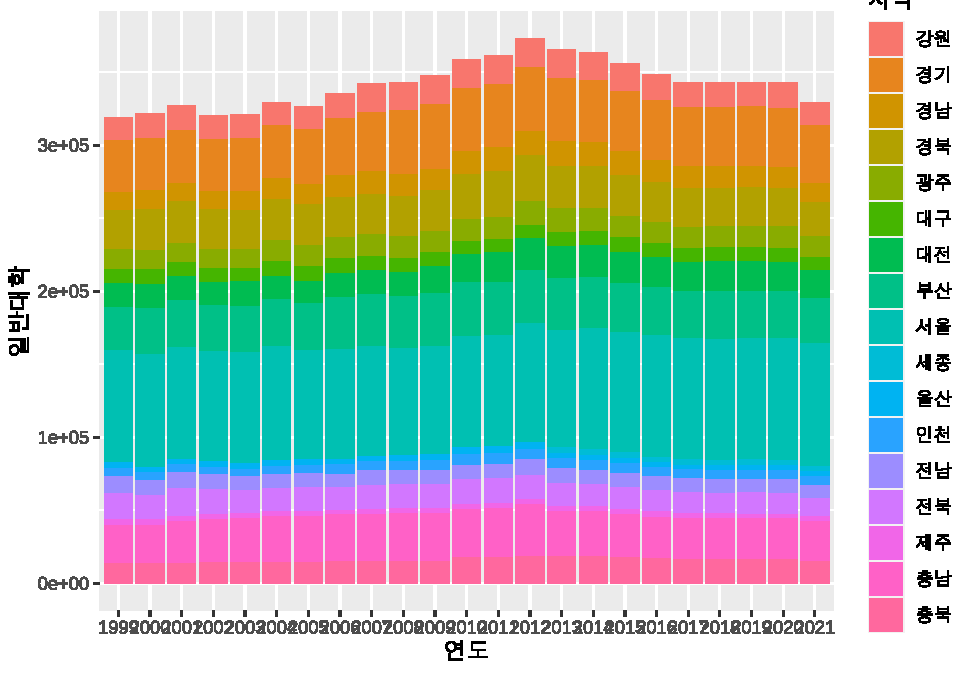
\includegraphics{chap3_files/figure-latex/unnamed-chunk-36-3.pdf}

2.3.2.2.2 \texttt{geom\_boxplot()}

박스 플롯은 데이터의 전반적 분포를 살펴볼 수 있는 매우 좋은 시각화 방법이다. 앞서 설명한 산점도는 X, Y축 모두 연속형 수치 변수를 사용하지만 박스 플롯은 이산형 변수로 분류되는 데이터의 전반적 분포를 시각화할 수 있다는 점에서 활용도가 크고 Scatter Plot에서는 표현할 수 없었던 중간값, IQR 범위, 이상치 등의 추가적인 정보를 같이 볼 수 있다는 장점이 있다. R에서 박스 플롯 레이어를 생성하기 위해서는 \texttt{geom\_boxplot()}을 사용한다.

박스 플롯으로 표현되는 상자의 중심은 중앙값이다. 중앙값은 가로선으로 표현되며 그 주위를 상자가 둘러싸고 있다. 상자의 상단과 하단은 관측값들의 25\%\textasciitilde75\%를 나타내고 중간 선은 전체 데이터의 중간값(50\%)을 표현한다. 상자의 상단과 하단 범위를 벗어나면 사분위 범위의 1.5배에 해당하는 '수염(whisker)'으로 표현된다. 수염 밖으로 존재하는 값은 점으로 표기하며 일반적으로 이상치로 간주한다. 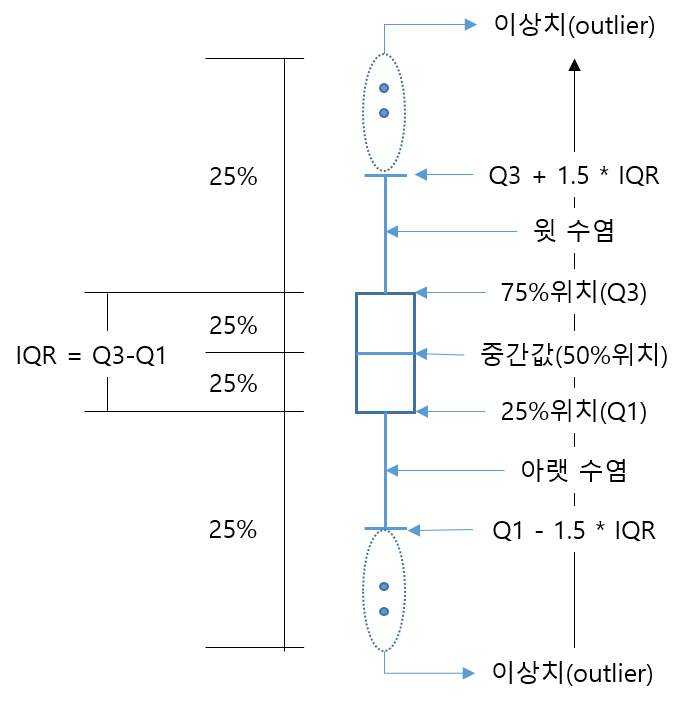
\includegraphics{boxplot.png}

\begin{Shaded}
\begin{Highlighting}[]
\FunctionTok{geom\_boxplot}\NormalTok{(}\AttributeTok{mapping =} \ConstantTok{NULL}\NormalTok{, }\AttributeTok{data =} \ConstantTok{NULL}\NormalTok{, }\AttributeTok{stat =} \StringTok{"boxplot"}\NormalTok{, }\AttributeTok{position =} \StringTok{"dodge2"}\NormalTok{, }\AttributeTok{outlier.color =} \ConstantTok{NULL}\NormalTok{, }\AttributeTok{outlier.fill =} \ConstantTok{NULL}\NormalTok{, }\AttributeTok{outlier.shape =} \DecValTok{19}\NormalTok{, }\AttributeTok{outlier.size =} \FloatTok{1.5}\NormalTok{, }\AttributeTok{outlier.stroke =} \FloatTok{0.5}\NormalTok{, }\AttributeTok{outlier.alpha =} \ConstantTok{NULL}\NormalTok{, }\AttributeTok{notch =} \ConstantTok{FALSE}\NormalTok{, }\AttributeTok{notchwidth =} \FloatTok{0.5}\NormalTok{, }\AttributeTok{na.rm =} \ConstantTok{FALSE}\NormalTok{, }\AttributeTok{show.legend =} \ConstantTok{NA}\NormalTok{, ...)}
  \SpecialCharTok{{-}}\NormalTok{ mapping }\SpecialCharTok{:} \FunctionTok{aes}\NormalTok{()를 사용하여 매핑할 미적요소, 생략되면 }\FunctionTok{ggplot}\NormalTok{()에 정의된 미적매핑 사용}
  \SpecialCharTok{{-}}\NormalTok{ data }\SpecialCharTok{:}\NormalTok{ 시각화를 위해 사용될 데이터, 생략되면 }\FunctionTok{ggplot}\NormalTok{()에 정의된 데이터 사용}
  \SpecialCharTok{{-}}\NormalTok{ stat }\SpecialCharTok{:}\NormalTok{ 시각화에 적용될 통계요소, 기본값은 }\StringTok{\textquotesingle{}boxplot\textquotesingle{}}
  \SpecialCharTok{{-}}\NormalTok{ position }\SpecialCharTok{:}\NormalTok{ 시각화에 적용될 위치요소, 기본값은 }\StringTok{\textquotesingle{}dodge2\textquotesingle{}}
  \SpecialCharTok{{-}}\NormalTok{ outlier.colour, outlier.color, outlier.fill, outlier.shape, outlier.size, outlier.stroke, outlier.alpha }\SpecialCharTok{:}\NormalTok{ 이상치로 표현되는 점의 미적요소 설정}
  \SpecialCharTok{{-}}\NormalTok{ notch }\SpecialCharTok{:}\NormalTok{ 상자의 중간값을 구분하는 귀퉁이를 표현할 지를 설정하기 위한 논리값(}\ConstantTok{TRUE}\SpecialCharTok{/}\ConstantTok{FALSE}\NormalTok{)}
  \SpecialCharTok{{-}}\NormalTok{ na.rm }\SpecialCharTok{:} \ConstantTok{NA}\NormalTok{ 값을 생략할 것인지를 설정하는 논리값(}\ConstantTok{TRUE}\SpecialCharTok{/}\ConstantTok{FALSE}\NormalTok{)}
  \SpecialCharTok{{-}}\NormalTok{ show.legend }\SpecialCharTok{:}\NormalTok{ 범례를 사용할 것인지를 설정하는 논리값(}\ConstantTok{TRUE}\SpecialCharTok{/}\ConstantTok{FALSE}\NormalTok{) }
\end{Highlighting}
\end{Shaded}

\texttt{geom\_boxplot()}에서 사용이 가능한 미적요소는 x, y, lower(xlower), upper(xupper), middle(xmiddle), ymin(xmin), ymax(xmax), alpha, colour, fill, group, linetype, shape, size, weight 등이 있다. 이 중 lower(xlower), upper(xupper), middle(xmiddle), ymin(xmin), ymax(xmax)는 박스를 수동으로 설정하기 위해 사용하는 미적요소이다.

\begin{Shaded}
\begin{Highlighting}[]
\DocumentationTok{\#\#  df\_취업통계 데이터를 ggplot 객체로 생성하고 p\_boxplot에 저장}
\NormalTok{p\_boxplot }\OtherTok{\textless{}{-}}\NormalTok{ df\_취업통계 }\SpecialCharTok{|}\ErrorTok{\textgreater{}}
  \FunctionTok{ggplot}\NormalTok{()}

\DocumentationTok{\#\# p\_boxplot에 x축에 대계열, y축에 취업률\_계로 매핑한 geom\_boxplot 레이어를 생성}
\NormalTok{p\_boxplot }\SpecialCharTok{+} 
  \FunctionTok{geom\_boxplot}\NormalTok{(}\FunctionTok{aes}\NormalTok{(}\AttributeTok{x =}\NormalTok{ 대계열, }\AttributeTok{y =}\NormalTok{ 취업률\_계)) }
\end{Highlighting}
\end{Shaded}

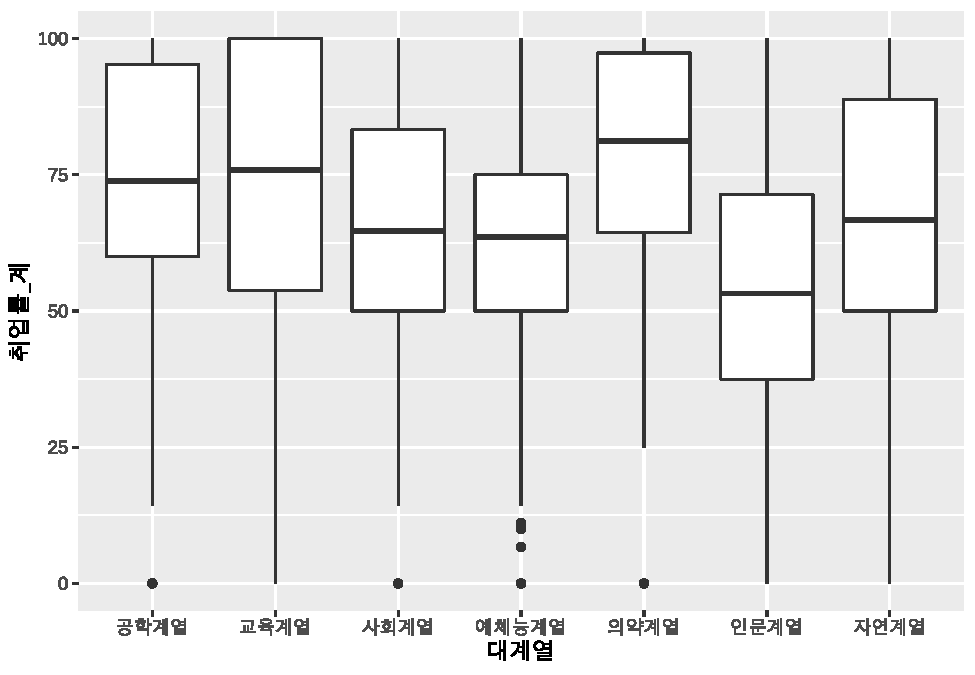
\includegraphics{chap3_files/figure-latex/unnamed-chunk-38-1.pdf}

\begin{Shaded}
\begin{Highlighting}[]
\DocumentationTok{\#\# p\_boxplot에 x축에 대계열, y축에 취업률\_계, fill을 대계열로 매핑, 미적요소를 설정한 geom\_boxplot레이어를 생성}
\NormalTok{p\_boxplot }\SpecialCharTok{+} 
  \FunctionTok{geom\_boxplot}\NormalTok{(}\FunctionTok{aes}\NormalTok{(}\AttributeTok{x =}\NormalTok{ 대계열, }\AttributeTok{y =}\NormalTok{ 취업률\_계, }\AttributeTok{fill =}\NormalTok{ 대계열), }\AttributeTok{linetype =} \DecValTok{2}\NormalTok{) }
\end{Highlighting}
\end{Shaded}

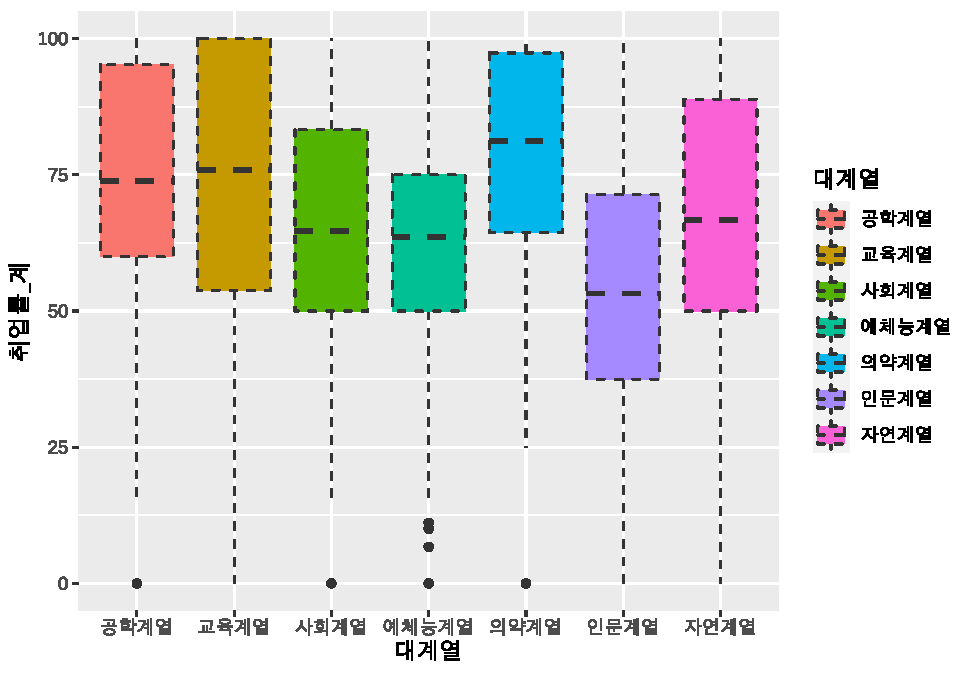
\includegraphics{chap3_files/figure-latex/unnamed-chunk-38-2.pdf}

\begin{Shaded}
\begin{Highlighting}[]
\DocumentationTok{\#\# p\_boxplot에 x축에 대계열, y축에 취업률\_계, fill을 대계열로 매핑, 미적요소를 설정한 geom\_boxplot레이어를 생성}
\NormalTok{p\_boxplot }\SpecialCharTok{+} 
  \FunctionTok{geom\_boxplot}\NormalTok{(}\FunctionTok{aes}\NormalTok{(}\AttributeTok{x =}\NormalTok{ 대계열, }\AttributeTok{y =}\NormalTok{ 취업률\_계, }\AttributeTok{fill =}\NormalTok{ 대계열), }\AttributeTok{linetype =} \DecValTok{2}\NormalTok{, }\AttributeTok{notch =} \ConstantTok{TRUE}\NormalTok{, }\AttributeTok{notchwidth =} \FloatTok{0.2}\NormalTok{, }\AttributeTok{outlier.shape =} \DecValTok{3}\NormalTok{) }
\end{Highlighting}
\end{Shaded}

\includegraphics{chap3_files/figure-latex/unnamed-chunk-38-3.pdf}

2.3.2.2.3 \texttt{geom\_violin()}

\texttt{geom\_violin()}은 박스플롯과 거의 유사한 시각화 방법인데 박스대신 데이터의 분포를 표현하는 바이올린과 유사한 형태의 도형으로 표현하는 시각화 방법이다. 박스 플롯에서는 25\%부터 75\%까지의 범위를 표현하는데 유용하지만 그 범위내에서 데이터가 어느 구간에 많이 분포되어 있는지는 표현하지 못한다. 이와 같은 단점을 극복하기 위해 \texttt{geom\_violin()}은 데이터가 많이 분포하는 구간은 좌우를 넓게 표현하고 데이터가 적게 분포하는 구간은 좌우를 좁게 표현해서 데이터의 전체 구간에 데이터의 분포를 시각화할 수 있다.

\begin{Shaded}
\begin{Highlighting}[]
\FunctionTok{geom\_violin}\NormalTok{(}\AttributeTok{mapping =} \ConstantTok{NULL}\NormalTok{, }\AttributeTok{data =} \ConstantTok{NULL}\NormalTok{, }\AttributeTok{stat =} \StringTok{"ydensity"}\NormalTok{, }\AttributeTok{position =} \StringTok{"dodge"}\NormalTok{, }\AttributeTok{draw\_quantiles =} \ConstantTok{NULL}\NormalTok{, }\AttributeTok{trim =} \ConstantTok{TRUE}\NormalTok{, }\AttributeTok{scale =} \StringTok{"area"}\NormalTok{, }\AttributeTok{na.rm =} \ConstantTok{FALSE}\NormalTok{, }\AttributeTok{show.legend =} \ConstantTok{NA}\NormalTok{, ...)}
  \SpecialCharTok{{-}}\NormalTok{ mapping }\SpecialCharTok{:} \FunctionTok{aes}\NormalTok{()를 사용하여 매핑할 미적요소, 생략되면 }\FunctionTok{ggplot}\NormalTok{()에 정의된 미적매핑 사용}
  \SpecialCharTok{{-}}\NormalTok{ data }\SpecialCharTok{:}\NormalTok{ 시각화를 위해 사용될 데이터, 생략되면 }\FunctionTok{ggplot}\NormalTok{()에 정의된 데이터 사용}
  \SpecialCharTok{{-}}\NormalTok{ stat }\SpecialCharTok{:}\NormalTok{ 시각화에 적용될 통계요소, 기본값은 }\StringTok{\textquotesingle{}ydensity\textquotesingle{}}
  \SpecialCharTok{{-}}\NormalTok{ position }\SpecialCharTok{:}\NormalTok{ 시각화에 적용될 위치요소, 기본값은 }\StringTok{\textquotesingle{}dodge\textquotesingle{}}
  \SpecialCharTok{{-}}\NormalTok{ draw\_quantiles }\SpecialCharTok{:}\NormalTok{ 박스플롯에서 표현하는 것과 같이 분위라인을 그리는데 사용될 분위 설정}
  \SpecialCharTok{{-}}\NormalTok{ trim }\SpecialCharTok{:}\NormalTok{ 끝부분을 잘라낼지 여부를 결정하는 논리값(}\ConstantTok{TRUE}\SpecialCharTok{/}\ConstantTok{FALSE}\NormalTok{)}
  \SpecialCharTok{{-}}\NormalTok{ scale }\SpecialCharTok{:}\NormalTok{ 데이터의 분포를 표현하는 도형의 크기를 표현하는 단위 설정, }\StringTok{\textquotesingle{}area\textquotesingle{}}\NormalTok{는 모든 도형의 크기를 동일하게 설정, }\StringTok{\textquotesingle{}count\textquotesingle{}}\NormalTok{는 데이터 개수에 따라 도형의 크기를 설정, }\StringTok{\textquotesingle{}width\textquotesingle{}}\NormalTok{는 모든 도형의 최대 너비를 동일하게 설정}
  \SpecialCharTok{{-}}\NormalTok{ na.rm }\SpecialCharTok{:} \ConstantTok{NA}\NormalTok{ 값을 생략할 것인지를 설정하는 논리값(}\ConstantTok{TRUE}\SpecialCharTok{/}\ConstantTok{FALSE}\NormalTok{)}
  \SpecialCharTok{{-}}\NormalTok{ show.legend }\SpecialCharTok{:}\NormalTok{ 범례를 사용할 것인지를 설정하는 논리값(}\ConstantTok{TRUE}\SpecialCharTok{/}\ConstantTok{FALSE}\NormalTok{) }
\end{Highlighting}
\end{Shaded}

\texttt{geom\_violin()} 에서 사용할 수 있는 미적요소는 x, y, alpha, color, fill, group, linetype, size, weight 등 이다.

\begin{Shaded}
\begin{Highlighting}[]
\DocumentationTok{\#\#  df\_취업통계 데이터를 ggplot 객체로 생성하고 p\_violin에 저장}
\NormalTok{p\_violin }\OtherTok{\textless{}{-}}\NormalTok{ df\_취업통계 }\SpecialCharTok{|}\ErrorTok{\textgreater{}}
  \FunctionTok{ggplot}\NormalTok{()}

\DocumentationTok{\#\# p\_violin에 x축에 대계열, y축에 취업률\_계로 매핑한 geom\_violin레이어를 생성}
\NormalTok{p\_violin }\SpecialCharTok{+} 
  \FunctionTok{geom\_violin}\NormalTok{(}\FunctionTok{aes}\NormalTok{(}\AttributeTok{x =}\NormalTok{ 대계열, }\AttributeTok{y =}\NormalTok{ 취업률\_계)) }
\end{Highlighting}
\end{Shaded}

\includegraphics{chap3_files/figure-latex/unnamed-chunk-40-1.pdf}

\begin{Shaded}
\begin{Highlighting}[]
\DocumentationTok{\#\# p\_violin에 x축에 대계열, y축에 취업률\_계로 매핑하고 0.25, 0.5, 0.75 위치에 선을 그림고 양쪽 끝을 자른 geom\_violin레이어를 생성}
\NormalTok{p\_violin }\SpecialCharTok{+} 
  \FunctionTok{geom\_violin}\NormalTok{(}\FunctionTok{aes}\NormalTok{(}\AttributeTok{x =}\NormalTok{ 대계열, }\AttributeTok{y =}\NormalTok{ 취업률\_계), }\AttributeTok{draw\_quantiles =} \FunctionTok{c}\NormalTok{(}\FloatTok{0.25}\NormalTok{, }\FloatTok{0.5}\NormalTok{, }\FloatTok{0.75}\NormalTok{), }\AttributeTok{trim =}\NormalTok{ F) }
\end{Highlighting}
\end{Shaded}

\includegraphics{chap3_files/figure-latex/unnamed-chunk-40-2.pdf}

\begin{Shaded}
\begin{Highlighting}[]
\DocumentationTok{\#\# p\_violin에 x축에 대계열, y축에 취업률\_계, color를 대계열로 매핑하고 선타입을 2로, 도형 표현 단위를 \textquotesingle{}count\textquotesingle{}로 설정한 geom\_violin레이어를 생성}
\NormalTok{p\_violin }\SpecialCharTok{+} 
  \FunctionTok{geom\_violin}\NormalTok{(}\FunctionTok{aes}\NormalTok{(}\AttributeTok{x =}\NormalTok{ 대계열, }\AttributeTok{y =}\NormalTok{ 취업률\_계, }\AttributeTok{fill =}\NormalTok{ 대계열), }\AttributeTok{linetype =} \DecValTok{2}\NormalTok{, }\AttributeTok{scale =} \StringTok{\textquotesingle{}count\textquotesingle{}}\NormalTok{) }
\end{Highlighting}
\end{Shaded}

\includegraphics{chap3_files/figure-latex/unnamed-chunk-40-3.pdf}

\hypertarget{uxb450uxac1cuxc758-uxc774uxc0b0uxd615-uxbcc0uxc218}{%
\subparagraph{2.3.2.3 두개의 이산형 변수}\label{uxb450uxac1cuxc758-uxc774uxc0b0uxd615-uxbcc0uxc218}}

X축과 Y축 모두 이산형 변수를 표현하고자 하는 경우는 X축과 Y축이 만나는 위치에 해당하는 데이터의 개수를 표현하는 방법이 거의 유일한 데이터 시각화 방법이다. 이를 위해 제공하는 함수가 \texttt{geom\_count()}이다. \texttt{geom\_count()}는 양 축의 교차되는 위치에 해당하는 데이터의 크기를 도형의 크기로 표현하는 시각화 방법이다.

\begin{Shaded}
\begin{Highlighting}[]
\FunctionTok{geom\_count}\NormalTok{(}\AttributeTok{mapping =} \ConstantTok{NULL}\NormalTok{, }\AttributeTok{data =} \ConstantTok{NULL}\NormalTok{, }\AttributeTok{stat =} \StringTok{"sum"}\NormalTok{, }\AttributeTok{position =} \StringTok{"identity"}\NormalTok{, }\AttributeTok{na.rm =} \ConstantTok{FALSE}\NormalTok{,}
  \AttributeTok{show.legend =} \ConstantTok{NA}\NormalTok{, ...)}
  \SpecialCharTok{{-}}\NormalTok{ mapping }\SpecialCharTok{:} \FunctionTok{aes}\NormalTok{()를 사용하여 매핑할 미적요소, 생략되면 }\FunctionTok{ggplot}\NormalTok{()에 정의된 미적매핑 사용}
  \SpecialCharTok{{-}}\NormalTok{ data }\SpecialCharTok{:}\NormalTok{ 시각화를 위해 사용될 데이터, 생략되면 }\FunctionTok{ggplot}\NormalTok{()에 정의된 데이터 사용}
  \SpecialCharTok{{-}}\NormalTok{ stat }\SpecialCharTok{:}\NormalTok{ 시각화에 적용될 통계요소, 기본값은 }\StringTok{\textquotesingle{}sum\textquotesingle{}}
  \SpecialCharTok{{-}}\NormalTok{ position }\SpecialCharTok{:}\NormalTok{ 시각화에 적용될 위치요소, 기본값은 }\StringTok{\textquotesingle{}identity\textquotesingle{}}
  \SpecialCharTok{{-}}\NormalTok{ na.rm }\SpecialCharTok{:} \ConstantTok{NA}\NormalTok{ 값을 생략할 것인지를 설정하는 논리값(}\ConstantTok{TRUE}\SpecialCharTok{/}\ConstantTok{FALSE}\NormalTok{)}
  \SpecialCharTok{{-}}\NormalTok{ show.legend }\SpecialCharTok{:}\NormalTok{ 범례를 사용할 것인지를 설정하는 논리값(}\ConstantTok{TRUE}\SpecialCharTok{/}\ConstantTok{FALSE}\NormalTok{) }
\end{Highlighting}
\end{Shaded}

\texttt{geom\_count()}에서 사용이 가능한 미적요소는 x, y, alpha, color, fill, group, shape, size, stroke 등 이다 .

\begin{Shaded}
\begin{Highlighting}[]
\DocumentationTok{\#\#  df\_취업통계 데이터를 ggplot 객체로 생성하고 p\_count에 저장}
\NormalTok{p\_count }\OtherTok{\textless{}{-}}\NormalTok{ df\_취업통계 }\SpecialCharTok{|}\ErrorTok{\textgreater{}} 
  \FunctionTok{ggplot}\NormalTok{()}

\DocumentationTok{\#\# p\_count에 x축에 대계열, y축에 학제를 매핑한 geom\_count레이어를 생성}
\NormalTok{p\_count }\SpecialCharTok{+} 
  \FunctionTok{geom\_count}\NormalTok{(}\FunctionTok{aes}\NormalTok{(}\AttributeTok{x =}\NormalTok{ 대계열, }\AttributeTok{y =}\NormalTok{ 학제))}
\end{Highlighting}
\end{Shaded}

\includegraphics{chap3_files/figure-latex/unnamed-chunk-42-1.pdf}

\hypertarget{uxc138uxac1cuxc758-uxc5f0uxc18duxd615-uxbcc0uxc218}{%
\paragraph{2.3.3 세개의 연속형 변수}\label{uxc138uxac1cuxc758-uxc5f0uxc18duxd615-uxbcc0uxc218}}

\texttt{ggplot}은 3차원 시각화는 지원하지 않는다. 하지만 3차원 공간을 2차원 평면에서 구현하는 방법을 제공한다. 그래서 X, Y, Z의 세 축으로 표현되는 3차원을 2차원으로 표현하기 위해서는 먼저 X, Y의 조합이 중복되지 않는 유일한 조합으로 설정되어야 하고 z값이 같은 위치들을 선으로 이어 등고선 형태로 이어주거나 해당 위치의 데이터 값을 색으로 표현하는 두가지 방법이 있다. 앞의 등고선을 사용하는 방법은 \texttt{geom\_contour()}를 사용하고 색으로 표현하는 방법은 \texttt{geom\_contour\_filled()}를 사용한다.

\begin{Shaded}
\begin{Highlighting}[]
\FunctionTok{geom\_contour}\NormalTok{(}\AttributeTok{mapping =} \ConstantTok{NULL}\NormalTok{, }\AttributeTok{data =} \ConstantTok{NULL}\NormalTok{, }\AttributeTok{stat =} \StringTok{"contour"}\NormalTok{, }\AttributeTok{position =} \StringTok{"identity"}\NormalTok{, }\AttributeTok{bins =} \ConstantTok{NULL}\NormalTok{, }\AttributeTok{binwidth =} \ConstantTok{NULL}\NormalTok{, }\AttributeTok{breaks =} \ConstantTok{NULL}\NormalTok{, }\AttributeTok{na.rm =} \ConstantTok{FALSE}\NormalTok{, }\AttributeTok{show.legend =} \ConstantTok{NA}\NormalTok{, ...)}
  \SpecialCharTok{{-}}\NormalTok{ mapping }\SpecialCharTok{:} \FunctionTok{aes}\NormalTok{()를 사용하여 매핑할 미적요소, 생략되면 }\FunctionTok{ggplot}\NormalTok{()에 정의된 미적매핑 사용}
  \SpecialCharTok{{-}}\NormalTok{ data }\SpecialCharTok{:}\NormalTok{ 시각화를 위해 사용될 데이터, 생략되면 }\FunctionTok{ggplot}\NormalTok{()에 정의된 데이터 사용}
  \SpecialCharTok{{-}}\NormalTok{ stat }\SpecialCharTok{:}\NormalTok{ 시각화에 적용될 통계요소, 기본값은 }\StringTok{\textquotesingle{}contour\textquotesingle{}}
  \SpecialCharTok{{-}}\NormalTok{ position }\SpecialCharTok{:}\NormalTok{ 시각화에 적용될 위치요소, 기본값은 }\StringTok{\textquotesingle{}identity\textquotesingle{}}
  \SpecialCharTok{{-}}\NormalTok{ bins }\SpecialCharTok{:}\NormalTok{ X축을 나누는 bin의 개수 설정}
  \SpecialCharTok{{-}}\NormalTok{ binwidth }\SpecialCharTok{:}\NormalTok{ X축을 나누는 bin의 너비 설정, 숫자벡터를 사용할 수 있다. (bin과 binwidth는 동시에 사용될 수 없다)}
  \SpecialCharTok{{-}}\NormalTok{ breaks }\SpecialCharTok{:}\NormalTok{ 등고선이 구분되는 수치 벡터 설정}
  \SpecialCharTok{{-}}\NormalTok{ na.rm }\SpecialCharTok{:} \ConstantTok{NA}\NormalTok{ 값을 생략할 것인지를 설정하는 논리값(}\ConstantTok{TRUE}\SpecialCharTok{/}\ConstantTok{FALSE}\NormalTok{)}
  \SpecialCharTok{{-}}\NormalTok{ show.legend }\SpecialCharTok{:}\NormalTok{ 범례를 사용할 것인지를 설정하는 논리값(}\ConstantTok{TRUE}\SpecialCharTok{/}\ConstantTok{FALSE}\NormalTok{) }
\end{Highlighting}
\end{Shaded}

\texttt{geom\_contour()}에서 사용이 가능한 미적요소는 x, y, alpha, color, group, linetype, size, weight 등 이다.

\begin{Shaded}
\begin{Highlighting}[]
\DocumentationTok{\#\#  df\_취업통계 데이터를 ggplot 객체로 생성하고 p\_contour에 저장}
\NormalTok{p\_contour }\OtherTok{\textless{}{-}}\NormalTok{ df\_취업통계 }\SpecialCharTok{|}\ErrorTok{\textgreater{}}
  \FunctionTok{ggplot}\NormalTok{()}

\DocumentationTok{\#\# p\_contour에 x축에 졸업자\_계, y축에 취업자\_합계\_계, z축에 취업률\_계를 매핑한 geom\_contour레이어를 생성}
\NormalTok{p\_contour }\SpecialCharTok{+} 
  \FunctionTok{geom\_contour}\NormalTok{(}\FunctionTok{aes}\NormalTok{(}\AttributeTok{x =}\NormalTok{ 졸업자\_계, }\AttributeTok{y =}\NormalTok{ 취업자\_합계\_계, }\AttributeTok{z =}\NormalTok{ 취업률\_계))}
\end{Highlighting}
\end{Shaded}

\includegraphics{chap3_files/figure-latex/unnamed-chunk-44-1.pdf}

\texttt{geom\_contour\_filled()}의 사용법과 주요 매개변수는 다음과 같다.

\begin{Shaded}
\begin{Highlighting}[]
\FunctionTok{geom\_contour\_filled}\NormalTok{(}\AttributeTok{mapping =} \ConstantTok{NULL}\NormalTok{, }\AttributeTok{data =} \ConstantTok{NULL}\NormalTok{, }\AttributeTok{stat =} \StringTok{"contour\_filled"}\NormalTok{, }\AttributeTok{position =} \StringTok{"identity"}\NormalTok{, }\AttributeTok{bins =} \ConstantTok{NULL}\NormalTok{, }\AttributeTok{binwidth =} \ConstantTok{NULL}\NormalTok{, }\AttributeTok{breaks =} \ConstantTok{NULL}\NormalTok{, }\AttributeTok{na.rm =} \ConstantTok{FALSE}\NormalTok{, }\AttributeTok{show.legend =} \ConstantTok{NA}\NormalTok{, ...)}
  \SpecialCharTok{{-}}\NormalTok{ mapping }\SpecialCharTok{:} \FunctionTok{aes}\NormalTok{()를 사용하여 매핑할 미적요소, 생략되면 }\FunctionTok{ggplot}\NormalTok{()에 정의된 미적매핑 사용}
  \SpecialCharTok{{-}}\NormalTok{ data }\SpecialCharTok{:}\NormalTok{ 시각화를 위해 사용될 데이터, 생략되면 }\FunctionTok{ggplot}\NormalTok{()에 정의된 데이터 사용}
  \SpecialCharTok{{-}}\NormalTok{ stat }\SpecialCharTok{:}\NormalTok{ 시각화에 적용될 통계요소, 기본값은 }\StringTok{\textquotesingle{}contour\_filled\textquotesingle{}}
  \SpecialCharTok{{-}}\NormalTok{ position }\SpecialCharTok{:}\NormalTok{ 시각화에 적용될 위치요소, 기본값은 }\StringTok{\textquotesingle{}identity\textquotesingle{}}
  \SpecialCharTok{{-}}\NormalTok{ bins }\SpecialCharTok{:}\NormalTok{ X축을 나누는 bin의 개수 설정}
  \SpecialCharTok{{-}}\NormalTok{ binwidth }\SpecialCharTok{:}\NormalTok{ X축을 나누는 bin의 너비 설정, 숫자벡터를 사용할 수 있다. (bin과 binwidth는 동시에 사용될 수 없다)}
  \SpecialCharTok{{-}}\NormalTok{ breaks }\SpecialCharTok{:}\NormalTok{ 등고선이 구분되는 수치 벡터 설정}
  \SpecialCharTok{{-}}\NormalTok{ na.rm }\SpecialCharTok{:} \ConstantTok{NA}\NormalTok{ 값을 생략할 것인지를 설정하는 논리값(}\ConstantTok{TRUE}\SpecialCharTok{/}\ConstantTok{FALSE}\NormalTok{)}
  \SpecialCharTok{{-}}\NormalTok{ show.legend }\SpecialCharTok{:}\NormalTok{ 범례를 사용할 것인지를 설정하는 논리값(}\ConstantTok{TRUE}\SpecialCharTok{/}\ConstantTok{FALSE}\NormalTok{) }
\end{Highlighting}
\end{Shaded}

\texttt{geom\_contour\_filled()}에서 사용이 가능한 미적요소는 x, y, alpha, color, group, linetype, size, subgroup 등 이다.

\begin{Shaded}
\begin{Highlighting}[]
\DocumentationTok{\#\#  df\_취업통계 데이터를 ggplot 객체로 생성하고 p\_contour\_filled에 저장}
\NormalTok{p\_contour\_filled }\OtherTok{\textless{}{-}}\NormalTok{ df\_취업통계 }\SpecialCharTok{|}\ErrorTok{\textgreater{}}
  \FunctionTok{ggplot}\NormalTok{()}

\DocumentationTok{\#\# p\_contour\_filled에 x축에 졸업자\_계, y축에 취업자\_합계\_계, z축에 취업률\_계를 매핑한 geom\_contour\_filled 레이어를 생성}
\NormalTok{p\_contour\_filled }\SpecialCharTok{+} 
  \FunctionTok{geom\_contour\_filled}\NormalTok{(}\FunctionTok{aes}\NormalTok{(}\AttributeTok{x =}\NormalTok{ 졸업자\_계, }\AttributeTok{y =}\NormalTok{ 취업자\_합계\_계, }\AttributeTok{z =}\NormalTok{ 취업률\_계))}
\end{Highlighting}
\end{Shaded}

\includegraphics{chap3_files/figure-latex/unnamed-chunk-46-1.pdf}

\hypertarget{uxad00uxce21uxce58-uxc5f0uxacb0}{%
\paragraph{2.3.4 관측치 연결}\label{uxad00uxce21uxce58-uxc5f0uxacb0}}

관측치 연결이 가장 많이 사용되는 데이터가 시계열 데이터이다. 시계열 데이터는 시간의 흐름에 따라 표현되는 데이터이다. 이 데이터는 보통 X축의 왼쪽에서 오른쪽으로 이동하면서 데이터가 표현된다. 따라서 X축에는 이산형 데이터로 표현되는 시간(연, 월, 일 등)이나 횟수가 매핑되고 하나의 X 변량에는 하나의 데이터만이 표현되어 이들 데이터들을 서로 연결하여 하나의 시계열 데이터를 생성한다. 보통 이 시계열 데이터는 선 그래프로 표현되는데 하나의 시각화에 여러개의 선으로 여러 시계열 데이터를 표현할 수도 있다.

\hypertarget{geom_line}{%
\subparagraph{\texorpdfstring{2.3.4.1 \texttt{geom\_line()}}{2.3.4.1 geom\_line()}}\label{geom_line}}

시계열 데이터를 표현하는 선 그래프를 시각화하는데 에는 \texttt{geom\_line()}이 사용된다.

\begin{Shaded}
\begin{Highlighting}[]
\FunctionTok{geom\_line}\NormalTok{(}\AttributeTok{mapping =} \ConstantTok{NULL}\NormalTok{, }\AttributeTok{data =} \ConstantTok{NULL}\NormalTok{, }\AttributeTok{stat =} \StringTok{"identity"}\NormalTok{, }\AttributeTok{position =} \StringTok{"identity"}\NormalTok{, }\AttributeTok{na.rm =} \ConstantTok{FALSE}\NormalTok{, }\AttributeTok{show.legend =} \ConstantTok{NA}\NormalTok{, ...)}
  \SpecialCharTok{{-}}\NormalTok{ mapping }\SpecialCharTok{:} \FunctionTok{aes}\NormalTok{()를 사용하여 매핑할 미적요소, 생략되면 }\FunctionTok{ggplot}\NormalTok{()에 정의된 미적매핑 사용}
  \SpecialCharTok{{-}}\NormalTok{ data }\SpecialCharTok{:}\NormalTok{ 시각화를 위해 사용될 데이터, 생략되면 }\FunctionTok{ggplot}\NormalTok{()에 정의된 데이터 사용}
  \SpecialCharTok{{-}}\NormalTok{ stat }\SpecialCharTok{:}\NormalTok{ 시각화에 적용될 통계요소, 기본값은 }\StringTok{\textquotesingle{}identity\textquotesingle{}}
  \SpecialCharTok{{-}}\NormalTok{ position }\SpecialCharTok{:}\NormalTok{ 시각화에 적용될 위치요소, , 기본값은 }\StringTok{\textquotesingle{}identity\textquotesingle{}}\NormalTok{로 권장됨}
  \SpecialCharTok{{-}}\NormalTok{ na.rm }\SpecialCharTok{:} \ConstantTok{NA}\NormalTok{ 값을 생략할 것인지를 설정하는 논리값(}\ConstantTok{TRUE}\SpecialCharTok{/}\ConstantTok{FALSE}\NormalTok{)}
  \SpecialCharTok{{-}}\NormalTok{ show.legend }\SpecialCharTok{:}\NormalTok{ 범례를 사용할 것인지를 설정하는 논리값(}\ConstantTok{TRUE}\SpecialCharTok{/}\ConstantTok{FALSE}\NormalTok{) }
\end{Highlighting}
\end{Shaded}

\texttt{geom\_line()}에서 사용이 가능한 미적요인은 x, y, alpha, color, group, linetype, size 등 이다.

\begin{Shaded}
\begin{Highlighting}[]
\DocumentationTok{\#\#  df\_입학자 데이터 중 지역이 전체가 아닌 데이터를 필터링하여 ggplot 객체로 생성하고 p\_line에 저장}
\NormalTok{p\_line }\OtherTok{\textless{}{-}}\NormalTok{ df\_입학자 }\SpecialCharTok{|}\ErrorTok{\textgreater{}} \FunctionTok{filter}\NormalTok{(지역 }\SpecialCharTok{!=} \StringTok{\textquotesingle{}전체\textquotesingle{}}\NormalTok{) }\SpecialCharTok{|}\ErrorTok{\textgreater{}}
  \FunctionTok{ggplot}\NormalTok{()}

\DocumentationTok{\#\#  p\_line객체에 x축에 연도, y축에 일반대학으로 매핑하고 각각의 line은 지역으로 그루핑하고, color는 지역으로 매핑한 geom\_line레이어를 생성}
\NormalTok{p\_line }\SpecialCharTok{+} 
  \FunctionTok{geom\_line}\NormalTok{(}\FunctionTok{aes}\NormalTok{(}\AttributeTok{x =}\NormalTok{ 연도, }\AttributeTok{y =}\NormalTok{ 일반대학, }\AttributeTok{group =}\NormalTok{ 지역, }\AttributeTok{color =}\NormalTok{ 지역))}
\end{Highlighting}
\end{Shaded}

\includegraphics{chap3_files/figure-latex/unnamed-chunk-48-1.pdf}

\hypertarget{geom_area}{%
\subparagraph{\texorpdfstring{2.3.4.2 \texttt{geom\_area()}}{2.3.4.2 geom\_area()}}\label{geom_area}}

\texttt{geom\_area()}는 \texttt{geom\_line()}과 유사한 선 그래프를 그린다. 다만 \texttt{geom\_line()}은 데이터를 연결하는 선만이 그려지는 반면 \texttt{geom\_area()}는 데이터를 연결한 선에서부터 X축까지의 면적을 색으로 채운다. 하지만 더 큰 차이는 여러 변량이 표현되는 다중 선 그래프의 경우 면적이 계속 쌓이는 방식으로 표현된다는 점이다.

\begin{Shaded}
\begin{Highlighting}[]
\FunctionTok{geom\_area}\NormalTok{(}\AttributeTok{mapping =} \ConstantTok{NULL}\NormalTok{, }\AttributeTok{data =} \ConstantTok{NULL}\NormalTok{, }\AttributeTok{stat =} \StringTok{"identity"}\NormalTok{, }\AttributeTok{position =} \StringTok{"stack"}\NormalTok{, }\AttributeTok{na.rm =} \ConstantTok{FALSE}\NormalTok{, }\AttributeTok{show.legend =} \ConstantTok{NA}\NormalTok{, }\AttributeTok{outline.type =} \StringTok{"upper"}\NormalTok{, ...)}
  \SpecialCharTok{{-}}\NormalTok{ mapping }\SpecialCharTok{:} \FunctionTok{aes}\NormalTok{()를 사용하여 매핑할 미적요소, 생략되면 }\FunctionTok{ggplot}\NormalTok{()에 정의된 미적매핑 사용}
  \SpecialCharTok{{-}}\NormalTok{ data }\SpecialCharTok{:}\NormalTok{ 시각화를 위해 사용될 데이터, 생략되면 }\FunctionTok{ggplot}\NormalTok{()에 정의된 데이터 사용}
  \SpecialCharTok{{-}}\NormalTok{ stat }\SpecialCharTok{:}\NormalTok{ 시각화에 적용될 통계요소, 기본값은 }\StringTok{\textquotesingle{}identity\textquotesingle{}}\NormalTok{으로 권장됨}
  \SpecialCharTok{{-}}\NormalTok{ position }\SpecialCharTok{:}\NormalTok{ 시각화에 적용될 위치요소, 기본값은 }\StringTok{\textquotesingle{}identity\textquotesingle{}}\NormalTok{로 권장됨}
  \SpecialCharTok{{-}}\NormalTok{ na.rm }\SpecialCharTok{:} \ConstantTok{NA}\NormalTok{ 값을 생략할 것인지를 설정하는 논리값(}\ConstantTok{TRUE}\SpecialCharTok{/}\ConstantTok{FALSE}\NormalTok{)}
  \SpecialCharTok{{-}}\NormalTok{ show.legend }\SpecialCharTok{:}\NormalTok{ 범례를 사용할 것인지를 설정하는 논리값(}\ConstantTok{TRUE}\SpecialCharTok{/}\ConstantTok{FALSE}\NormalTok{) }
\end{Highlighting}
\end{Shaded}

\texttt{geom\_area()}에서 사용이 가능한 미적요인은 x, y, alpha, color, fill, group, linetype, size 등 이다.

\begin{Shaded}
\begin{Highlighting}[]
\DocumentationTok{\#\#  df\_입학자 데이터 중 지역이 전체가 아닌 데이터를 필터링하여 ggplot 객체로 생성하고 p\_area에 저장}
\NormalTok{p\_area }\OtherTok{\textless{}{-}}\NormalTok{ df\_입학자 }\SpecialCharTok{|}\ErrorTok{\textgreater{}} \FunctionTok{filter}\NormalTok{(지역 }\SpecialCharTok{!=} \StringTok{\textquotesingle{}전체\textquotesingle{}}\NormalTok{) }\SpecialCharTok{|}\ErrorTok{\textgreater{}}
  \FunctionTok{ggplot}\NormalTok{()}

\DocumentationTok{\#\#  p\_line객체에 x축에 연도, y축에 일반대학으로 매핑하고 각각의 line은 지역으로 그루핑하고, fill는 지역으로 매핑한 geom\_line 레이어를 생성}
\NormalTok{p\_area }\SpecialCharTok{+} 
  \FunctionTok{geom\_area}\NormalTok{(}\FunctionTok{aes}\NormalTok{(}\AttributeTok{x =}\NormalTok{ 연도, }\AttributeTok{y =}\NormalTok{ 일반대학, }\AttributeTok{group =}\NormalTok{ 지역, }\AttributeTok{fill =}\NormalTok{ 지역))}
\end{Highlighting}
\end{Shaded}

\includegraphics{chap3_files/figure-latex/unnamed-chunk-50-1.pdf}

\hypertarget{uxd1b5uxacc4-uxbcc0uxd658-uxc694uxc18cstat}{%
\paragraph{\texorpdfstring{2.3.4 통계 변환 요소(\texttt{stat})}{2.3.4 통계 변환 요소(stat)}}\label{uxd1b5uxacc4-uxbcc0uxd658-uxc694uxc18cstat}}

앞서 설명한 기하요소 중에 산점도와 같은 시각화는 데이터의 자체 값을 사용하는 기하요소이고 히스토그램과 같은 시각화는 데이터를 통계 처리한 후 그 결과를 사용하였다. 사실 데이터 자체값을 그대로 사용하는 경우에도 함수의 매개변수로 통계 변환을 뜻하는 매개변수인 \texttt{stat}을 \texttt{identity}로 설정함으로서 그 자체값을 사용하는 통계변환을 지정한다. 따라서 모든 기하요소에는 기본적으로 디폴트 통계 변환 요소가 포함된다.\\
\includegraphics{stat.png}

\hypertarget{stat_}{%
\subparagraph{\texorpdfstring{2.3.4.1 \texttt{stat\_*()}}{2.3.4.1 stat\_*()}}\label{stat_}}

\texttt{ggplot}를 사용하는 사용자들은 주로 \texttt{geom\_*} 함수를 사용하여 시각화의 주요 데이터 레이어를 를 생성한다. 하지만 \texttt{stat\_*()} 함수를 사용하여 데이터 레이어를 생성할 수도 있다. 모든 \texttt{geom\_*()} 로 생성된 레이어는 \texttt{stat\_*()} 사용하여 동일한 레이어를 생성할 수 있다. 다시 말하자면 \texttt{geom\_*()}은 데이터가 표현될 도형을 위주로 시각화 레이어를 생성하는 방법이고 \texttt{stat\_*()}은 데이터의 통계적 변환을 위주로 시각화 레이어를 생성하는 방법이다.

\texttt{stat\_*()}을 사용하여 \texttt{geom\_*()}과 동일한 데이터 레이어를 생성하는 방법은 생각보다 간단하다. \texttt{geom\_*()}의 모든 함수에는 \texttt{stat\ =} 이라는 매개변수가 있다. 이 매개변수를 \texttt{stat\_} 다음에 붙여주고 \texttt{stat\_*()} 매개변수에 \texttt{geom\ =}에 기하요소 이름을 넣어주면 된다. 이 명명 법칙이 일부 적용되지 않는 함수도 있지만 대부분 아래의 그림과 같이 적용이 가능하다.

\includegraphics{stat1.png}

\begin{Shaded}
\begin{Highlighting}[]
\DocumentationTok{\#\# geom\_histogram()과 동일한 결과}
\NormalTok{p\_histogram }\SpecialCharTok{+} \FunctionTok{stat\_bin}\NormalTok{(}\FunctionTok{aes}\NormalTok{(}\AttributeTok{x =}\NormalTok{ 취업률\_계), }\AttributeTok{geom =} \StringTok{\textquotesingle{}bar\textquotesingle{}}\NormalTok{)}
\end{Highlighting}
\end{Shaded}

\includegraphics{chap3_files/figure-latex/unnamed-chunk-51-1.pdf}

\begin{Shaded}
\begin{Highlighting}[]
\DocumentationTok{\#\# geom\_freqpoly()과 동일한 결과}
\NormalTok{p\_density }\SpecialCharTok{+} 
  \FunctionTok{stat\_bin}\NormalTok{(}\FunctionTok{aes}\NormalTok{(}\AttributeTok{x =}\NormalTok{ 취업률\_계), }\AttributeTok{geom =} \StringTok{\textquotesingle{}line\textquotesingle{}}\NormalTok{)}
\end{Highlighting}
\end{Shaded}

\includegraphics{chap3_files/figure-latex/unnamed-chunk-51-2.pdf}

\begin{Shaded}
\begin{Highlighting}[]
\DocumentationTok{\#\# geom\_density()과 동일한 결과}
\NormalTok{p\_density }\SpecialCharTok{+} 
  \FunctionTok{stat\_density}\NormalTok{(}\FunctionTok{aes}\NormalTok{(}\AttributeTok{x =}\NormalTok{ 취업률\_계), }\AttributeTok{geom =} \StringTok{\textquotesingle{}line\textquotesingle{}}\NormalTok{)}
\end{Highlighting}
\end{Shaded}

\includegraphics{chap3_files/figure-latex/unnamed-chunk-51-3.pdf}

\begin{Shaded}
\begin{Highlighting}[]
\DocumentationTok{\#\# geom\_point()과 동일한 결과}
\NormalTok{p\_point }\SpecialCharTok{+} \FunctionTok{stat\_identity}\NormalTok{(}\FunctionTok{aes}\NormalTok{(}\AttributeTok{x =}\NormalTok{ 졸업자\_계, }\AttributeTok{y =}\NormalTok{ 취업자\_합계\_계), }\AttributeTok{geom =} \StringTok{\textquotesingle{}point\textquotesingle{}}\NormalTok{)}
\end{Highlighting}
\end{Shaded}

\includegraphics{chap3_files/figure-latex/unnamed-chunk-51-4.pdf}

\begin{Shaded}
\begin{Highlighting}[]
\DocumentationTok{\#\# geom\_text()과 동일한 결과}
\NormalTok{p\_text }\SpecialCharTok{+}
  \FunctionTok{stat\_identity}\NormalTok{(}\FunctionTok{aes}\NormalTok{(}\AttributeTok{x =}\NormalTok{ 연도, }\AttributeTok{y =}\NormalTok{ 전문대학), }\AttributeTok{geom =} \StringTok{\textquotesingle{}point\textquotesingle{}}\NormalTok{) }\SpecialCharTok{+}
  \FunctionTok{stat\_identity}\NormalTok{(}\FunctionTok{aes}\NormalTok{(}\AttributeTok{x =}\NormalTok{ 연도, }\AttributeTok{y =}\NormalTok{ 전문대학, }\AttributeTok{label =}\NormalTok{ 전문대학), }\AttributeTok{geom =} \StringTok{\textquotesingle{}text\textquotesingle{}}\NormalTok{)}
\end{Highlighting}
\end{Shaded}

\includegraphics{chap3_files/figure-latex/unnamed-chunk-51-5.pdf}

\begin{Shaded}
\begin{Highlighting}[]
\DocumentationTok{\#\# geom\_label()과 동일한 결과}
\NormalTok{p\_label }\SpecialCharTok{+}
  \FunctionTok{stat\_identity}\NormalTok{(}\FunctionTok{aes}\NormalTok{(}\AttributeTok{x =}\NormalTok{ 연도, }\AttributeTok{y =}\NormalTok{ 전문대학, }\AttributeTok{label =}\NormalTok{ 전문대학), }\AttributeTok{geom =} \StringTok{\textquotesingle{}label\textquotesingle{}}\NormalTok{)}
\end{Highlighting}
\end{Shaded}

\includegraphics{chap3_files/figure-latex/unnamed-chunk-51-6.pdf}

\begin{Shaded}
\begin{Highlighting}[]
\DocumentationTok{\#\# geom\_smooth()과 동일한 결과}
\NormalTok{p\_smooth }\SpecialCharTok{+} 
  \FunctionTok{stat\_identity}\NormalTok{(}\FunctionTok{aes}\NormalTok{(}\AttributeTok{x =}\NormalTok{ 연도, }\AttributeTok{y =}\NormalTok{ 전문대학), }\AttributeTok{geom =} \StringTok{\textquotesingle{}point\textquotesingle{}}\NormalTok{) }\SpecialCharTok{+}
  \FunctionTok{stat\_smooth}\NormalTok{(}\FunctionTok{aes}\NormalTok{(}\AttributeTok{x =}\NormalTok{ 연도, }\AttributeTok{y =}\NormalTok{ 전문대학, }\AttributeTok{group =} \DecValTok{1}\NormalTok{), }\AttributeTok{method =} \StringTok{\textquotesingle{}loess\textquotesingle{}}\NormalTok{, }\AttributeTok{geom =} \StringTok{\textquotesingle{}smooth\textquotesingle{}}\NormalTok{)}
\end{Highlighting}
\end{Shaded}

\includegraphics{chap3_files/figure-latex/unnamed-chunk-51-7.pdf}

\begin{Shaded}
\begin{Highlighting}[]
\DocumentationTok{\#\# geom\_col()과 동일한 결과}
\NormalTok{p\_col }\SpecialCharTok{+}
  \FunctionTok{stat\_identity}\NormalTok{(}\FunctionTok{aes}\NormalTok{(}\AttributeTok{x =}\NormalTok{ 연도, }\AttributeTok{y =}\NormalTok{ 일반대학), }\AttributeTok{geom =} \StringTok{\textquotesingle{}bar\textquotesingle{}}\NormalTok{)}
\end{Highlighting}
\end{Shaded}

\includegraphics{chap3_files/figure-latex/unnamed-chunk-51-8.pdf}

\begin{Shaded}
\begin{Highlighting}[]
\DocumentationTok{\#\# geom\_boxplot()과 동일한 결과}
\NormalTok{p\_boxplot }\SpecialCharTok{+} 
  \FunctionTok{stat\_boxplot}\NormalTok{(}\FunctionTok{aes}\NormalTok{(}\AttributeTok{x =}\NormalTok{ 대계열, }\AttributeTok{y =}\NormalTok{ 취업률\_계)) }
\end{Highlighting}
\end{Shaded}

\includegraphics{chap3_files/figure-latex/unnamed-chunk-51-9.pdf}

\begin{Shaded}
\begin{Highlighting}[]
\DocumentationTok{\#\# geom\_violin()과 동일한 결과}
\NormalTok{p\_violin }\SpecialCharTok{+} 
  \FunctionTok{stat\_ydensity}\NormalTok{(}\FunctionTok{aes}\NormalTok{(}\AttributeTok{x =}\NormalTok{ 대계열, }\AttributeTok{y =}\NormalTok{ 취업률\_계)) }
\end{Highlighting}
\end{Shaded}

\includegraphics{chap3_files/figure-latex/unnamed-chunk-51-10.pdf}

\begin{Shaded}
\begin{Highlighting}[]
\DocumentationTok{\#\# geom\_line()과 동일한 결과}
\NormalTok{p\_line }\SpecialCharTok{+} 
  \FunctionTok{stat\_identity}\NormalTok{(}\FunctionTok{aes}\NormalTok{(}\AttributeTok{x =}\NormalTok{ 연도, }\AttributeTok{y =}\NormalTok{ 일반대학, }\AttributeTok{group =}\NormalTok{ 지역, }\AttributeTok{color =}\NormalTok{ 지역), }\AttributeTok{geom =} \StringTok{\textquotesingle{}line\textquotesingle{}}\NormalTok{)}
\end{Highlighting}
\end{Shaded}

\includegraphics{chap3_files/figure-latex/unnamed-chunk-51-11.pdf}

\begin{Shaded}
\begin{Highlighting}[]
\DocumentationTok{\#\# geom\_area()과 동일한 결과}
\NormalTok{p\_area }\SpecialCharTok{+} 
  \FunctionTok{stat\_identity}\NormalTok{(}\FunctionTok{aes}\NormalTok{(}\AttributeTok{x =}\NormalTok{ 연도, }\AttributeTok{y =}\NormalTok{ 일반대학, }\AttributeTok{group =}\NormalTok{ 지역, }\AttributeTok{fill =}\NormalTok{ 지역), }\AttributeTok{geom =} \StringTok{\textquotesingle{}area\textquotesingle{}}\NormalTok{, }\AttributeTok{position =} \StringTok{\textquotesingle{}stack\textquotesingle{}}\NormalTok{)}
\end{Highlighting}
\end{Shaded}

\includegraphics{chap3_files/figure-latex/unnamed-chunk-51-12.pdf}

위에서 살펴본 바와 같이 \texttt{geom\_*()}으로 생성할 수 있는 기하요소 레이어는 \texttt{stat\_*()}을 사용하여 동일하게 생성할 수 있다. 하지만 \texttt{geom\_*()}에서는 제공하지 않는 \texttt{stat\_*()}에서만 제공하는 특별한 레이어가 있다.

\hypertarget{stat_summary}{%
\subparagraph{\texorpdfstring{2.3.4.2 \texttt{stat\_summary()}}{2.3.4.2 stat\_summary()}}\label{stat_summary}}

\texttt{geom\_*()}으로 생성한 기하요소 레이어에 통계적으로 변환된 데이터를 추가적으로 표현해야 할 경우가 있다. 가장 대표적인 예가 박스 플롯에서 중간값이 자동적으로 표현되지만 평균값을 추가적으로 표현해야 하는 경우가 있다. 이런 경우에 대비하여 특정 함수로 요약한 통계치를 표현하는 레이어를 추가할 때 \texttt{stat\_summary()}를 사용한다.

\begin{Shaded}
\begin{Highlighting}[]
\FunctionTok{stat\_summary}\NormalTok{(}\AttributeTok{mapping =} \ConstantTok{NULL}\NormalTok{, }\AttributeTok{data =} \ConstantTok{NULL}\NormalTok{, }\AttributeTok{geom =} \StringTok{"pointrange"}\NormalTok{, }\AttributeTok{position =} \StringTok{"identity"}\NormalTok{, }\AttributeTok{fun.data =} \ConstantTok{NULL}\NormalTok{, }\AttributeTok{fun =} \ConstantTok{NULL}\NormalTok{, }\AttributeTok{fun.max =} \ConstantTok{NULL}\NormalTok{, }\AttributeTok{fun.min =} \ConstantTok{NULL}\NormalTok{, }\AttributeTok{fun.args =} \FunctionTok{list}\NormalTok{(), }\AttributeTok{na.rm =} \ConstantTok{FALSE}\NormalTok{, }\AttributeTok{show.legend =} \ConstantTok{NA}\NormalTok{, fun.y, fun.ymin, fun.ymax)}
  \SpecialCharTok{{-}}\NormalTok{ mapping }\SpecialCharTok{:} \FunctionTok{aes}\NormalTok{()를 사용하여 매핑할 미적요소, 생략되면 }\FunctionTok{ggplot}\NormalTok{()에 정의된 미적매핑 사용}
  \SpecialCharTok{{-}}\NormalTok{ data }\SpecialCharTok{:}\NormalTok{ 시각화를 위해 사용될 데이터, 생략되면 }\FunctionTok{ggplot}\NormalTok{()에 정의된 데이터 사용}
  \SpecialCharTok{{-}}\NormalTok{ geom }\SpecialCharTok{:}\NormalTok{ 시각화에 적용될 미적요소를 설정, 기본값은 }\StringTok{\textquotesingle{}pointrange\textquotesingle{}}
  \SpecialCharTok{{-}}\NormalTok{ position }\SpecialCharTok{:}\NormalTok{ 시각화에 적용될 위치요소 설정, 기본값은 }\StringTok{\textquotesingle{}identity\textquotesingle{}}
  \SpecialCharTok{{-}}\NormalTok{ fun.data }\SpecialCharTok{:}\NormalTok{ ymin, y, ymax를 포함하는 데이터프레임을 반환하는 함수 설정}
  \SpecialCharTok{{-}}\NormalTok{ fun, fun.y }\SpecialCharTok{:}\NormalTok{ X값에 대응하는 Y값을 구하는 함수 설정}
  \SpecialCharTok{{-}}\NormalTok{ fun.min, fun.ymin }\SpecialCharTok{:}\NormalTok{ X에 대응하는 Y값의 최소값 함수 설정}
  \SpecialCharTok{{-}}\NormalTok{ fun.max, fun.ymax }\SpecialCharTok{:}\NormalTok{  X에 대응하는 Y값의 최대값 함수 설정}
  \SpecialCharTok{{-}}\NormalTok{ fun.args }\SpecialCharTok{:}\NormalTok{ 함수에 전달될 }
  \SpecialCharTok{{-}}\NormalTok{ na.rm }\SpecialCharTok{:} \ConstantTok{NA}\NormalTok{ 값을 생략할 것인지를 설정하는 논리값(}\ConstantTok{TRUE}\SpecialCharTok{/}\ConstantTok{FALSE}\NormalTok{)}
  \SpecialCharTok{{-}}\NormalTok{ show.legend }\SpecialCharTok{:}\NormalTok{ 범례를 사용할 것인지를 설정하는 논리값(}\ConstantTok{TRUE}\SpecialCharTok{/}\ConstantTok{FALSE}\NormalTok{) }
\end{Highlighting}
\end{Shaded}

아래의 코드는 박스 플롯에 평균을 추가하는 코드이다.

\begin{Shaded}
\begin{Highlighting}[]
\DocumentationTok{\#\# p\_boxplot에 geom\_boxplot 레이어를 만들고 X값에 대한 Y 값은 평균(mean), 미적요소는 point, color는 \textquotesingle{}red\textquotesingle{}로 설정한 stat\_summary 레이어를 추가}
\NormalTok{p\_boxplot }\SpecialCharTok{+} 
  \FunctionTok{geom\_boxplot}\NormalTok{(}\FunctionTok{aes}\NormalTok{(}\AttributeTok{x =}\NormalTok{ 대계열, }\AttributeTok{y =}\NormalTok{ 취업률\_계)) }\SpecialCharTok{+}
  \FunctionTok{stat\_summary}\NormalTok{(}\FunctionTok{aes}\NormalTok{(}\AttributeTok{x =}\NormalTok{ 대계열, }\AttributeTok{y =}\NormalTok{ 취업률\_계), }\AttributeTok{fun =} \StringTok{\textquotesingle{}mean\textquotesingle{}}\NormalTok{, }\AttributeTok{geom =} \StringTok{\textquotesingle{}point\textquotesingle{}}\NormalTok{, }\AttributeTok{color =} \StringTok{\textquotesingle{}red\textquotesingle{}}\NormalTok{)}
\end{Highlighting}
\end{Shaded}

\includegraphics{chap3_files/figure-latex/unnamed-chunk-53-1.pdf}

\begin{Shaded}
\begin{Highlighting}[]
\DocumentationTok{\#\# p\_point에 geom\_point 레이어를 만들고 X값에 대한 Y 값은 평균(mean), 미적요소는 point, color는 \textquotesingle{}red\textquotesingle{}로 설정한 레이어와 stat\_summary 레이어를 추가하는데 X값에 대한 Y 값은 평균(mean), 미적요소는 point, color는 \textquotesingle{}red\textquotesingle{}로 설정한 레이어를 추가 }
\NormalTok{p\_point }\SpecialCharTok{+} 
  \FunctionTok{geom\_point}\NormalTok{(}\FunctionTok{aes}\NormalTok{(}\AttributeTok{x =}\NormalTok{ 대계열, }\AttributeTok{y =}\NormalTok{ 취업률\_계), }\AttributeTok{alpha =} \FloatTok{0.1}\NormalTok{) }\SpecialCharTok{+}
  \FunctionTok{stat\_summary}\NormalTok{(}\FunctionTok{aes}\NormalTok{(}\AttributeTok{x =}\NormalTok{ 대계열, }\AttributeTok{y =}\NormalTok{ 취업률\_계), }\AttributeTok{fun =} \StringTok{\textquotesingle{}mean\textquotesingle{}}\NormalTok{, }\AttributeTok{geom =} \StringTok{\textquotesingle{}point\textquotesingle{}}\NormalTok{, }\AttributeTok{color =} \StringTok{\textquotesingle{}red\textquotesingle{}}\NormalTok{, }\AttributeTok{size =} \DecValTok{3}\NormalTok{) }\SpecialCharTok{+}
    \FunctionTok{stat\_summary}\NormalTok{(}\FunctionTok{aes}\NormalTok{(}\AttributeTok{x =}\NormalTok{ 대계열, }\AttributeTok{y =}\NormalTok{ 취업률\_계), }\AttributeTok{fun =} \StringTok{\textquotesingle{}median\textquotesingle{}}\NormalTok{, }\AttributeTok{geom =} \StringTok{\textquotesingle{}point\textquotesingle{}}\NormalTok{, }\AttributeTok{color =} \StringTok{\textquotesingle{}blue\textquotesingle{}}\NormalTok{, }\AttributeTok{size =} \DecValTok{3}\NormalTok{)}
\end{Highlighting}
\end{Shaded}

\includegraphics{chap3_files/figure-latex/unnamed-chunk-53-2.pdf}

\end{document}
